\documentclass{scrreprt}
\usepackage{amssymb}
\usepackage{mathtools}
\usepackage{dsfont}
% \usepackage{hyperref}
\usepackage{graphicx}
\usepackage{caption}
\usepackage{subcaption}
\usepackage{pgfplots}

\pgfplotsset{compat=1.12}
\pgfplotsset{soldot/.style={color=blue,only marks,mark=*}}
\pgfplotsset{holdot/.style={color=blue,fill=white,only marks,mark=*}}

% Set counter for section
\setcounter{section}{1}

% new commands
\newcommand{\qed}{$\hfill\blacksquare$}
% new commands (end)

% new theorems
\newtheorem{theorem}{Theorem}[chapter]
\newtheorem{lemma}[theorem]{Lemma}
\newtheorem{proposition}[theorem]{Proposition}
\newtheorem{corollary}[theorem]{Corollary}
\newtheorem{definition}[theorem]{Definition}
\newtheorem{example}[theorem]{Example}
\newtheorem{remark}[theorem]{Remark}
\newtheorem{algorithm}[theorem]{Algorithm}
% new theorems (end)

% new environments
\newenvironment{proof}[1][Proof]{\begin{trivlist}
\item[\hskip \labelsep {\bfseries #1}]}{\end{trivlist}}
\newenvironment{describe}[1][]{\begin{trivlist}
\item[\hskip \labelsep {\bfseries #1}]\itshape}{\end{trivlist}}
% new environments (end)

\begin{document}

\pagenumbering{Roman} % set page numbering to Roman

% title_page
\begin{titlepage} % (fold)

    \begin{center}
        \begin{Large}
            Universit\"at Regensburg\\
            Fakult\"at f\"ur Mathematik\\
        \end{Large}
        \vspace{1cm}
        \begin{Large}
            \textbf{VARIATIONAL METHODS IN IMAGE PROCESSING USING A FAST PRIMAL-DUAL ALGORITHM}
        \end{Large}
        \vspace{1cm}
        \begin{center}
        
\includegraphics[width=8cm]{img/sigillum.png}
        \vspace{1cm}\\
        \begin{Large}
            \textbf{MASTERARBEIT}\\
        \end{Large}
        \vspace{0.5cm}
        \begin{large}
            zur Erlangung des akademischen Grades\\
            Master of Science\\
            im Studiengang Computational Science\\
            \vspace{0.5cm}
            Eingereicht bei Prof. Dr. Harald Garcke\\
            am 28.02.2016
        \end{large}
        \vspace{0.5cm}
    \end{center}

    \begin{flushleft}
        \begin{large}
            Vorgelegt von:\\
            Michael Bauer\\
            Banater Str. 1\\
            84061 Ergolsbach\\
            Geboren am 23.08.1987 in Gr\"afelfing
            % Matrikelnummer: 152 8558
        \end{large}
    \end{flushleft}

    \end{center}

\end{titlepage}
% title_page (end)

\newpage
\chapter*{Abstract} % (fold)
\label{cha:abstract}

    We present a comparison of different convex total variation based image processing algorithms and the non-convex Mumford-Shah Functional. We will revisit and make use of the fast primal-dual algorithm of \cite{Pock-et-al-iccv09}. We consider all steps, projections, operators and computations and will give a range of proofs. We also present a various range of applications and compare the presented methods to each other. Providing run-times, used memory and results will lead us to a conclusion which problem fits best to several situations. 
    
% chapter abstract (end)

\newpage
% \chapter*{Acknowledgements} % (fold)
% \label{cha:acknowledgements}
    
% chapter acknowledgements (end)

% \newpage

% Content, Tables, Figures
\tableofcontents
\listoftables
\listoffigures

\pagenumbering{arabic} % set page numbering back to arabic
\chapter{Introduction} % (fold)
\label{cha:introduction}

    In the second decade of the twenty-first century autonomous driving seems to be the big thing for the Car, Computer and Software industry. The expectation is nothing less than having fewer, or even no, accidents. With these cars, industry is trying to change the world to a better. As this may comfort many people, it poses a lot of problems which need to be solved, for instance a stable hardware or even more important viable software. One field of research - of many others - is called Machine Learning, where the computer is trained to make the right decisions in the right situations. The car should be able to accommodate to all possible circumstances which could appear during a drive. To make it even more complicated, the car would need to take a decision in real-time. As one can imagine, it is extremely difficult to develop fast, stable and tractable methods.\\
    Learning from a certain situation, the car and the computer respectively needs data from the environment. This can be the shape of another car, traffic lights, differences in the lighting conditions or the distance to other objects. What all these information have in common, they can be collected via images. Small cameras are tracking the traffic and surrounding and providing data. Using the images, the car's computer can be trained when to stop or where to turn right.\\
    But it's not only the autonomously driving cars which make use of images to learn. Doctors use X-ray view or MRI scans in patient treatment, semiconductor companies use pictures of wafers seeking for damages on it, e.g. scratches or dark spots and unfortunately images are also used in modern warfare. For this reason image processing has become more important during the last decades. Researchers dealt with many problems like edge detection, deblurring, denoising, inpainting or image segmentation. In the field of edge detection the probably most famous researcher is John F. Canny. He provided the first tractable and stable edge detection algorithm, presented in the year 1986 (reference). One step in Canny's edge detector is to denoise and smooth the image. Therefore a Gaussian-Filter is used. The idea behind this filter is to convolute an image with a Gaussian kernel, or also called Gaussian curve. This filter provides reasonable results, but no more no less.\\
    Only three years after Canny published his work, two researchers, namely David Mumford and Jayant Shah, published a paper whose impact continous to this day - to date it was cited over 4.500 times (scholar). They proposed to minimize the energy of the so called Mumford-Shah Functional in order to approximate an image optimally. Solving this optimization problem leads to applications like image denoising, inpainting and even segmentation could be handled. Unfortunately, this functional is by definition non-convex. For this reason finding the minimal energy of it is a NP-hard problem. This fact makes it so difficult to deal with but also so interesting.\\
    One approach to compute the minimizer is by convex relaxation. It makes the non-convex problem convex and one can apply a fast and tractable algorithm. The idea of convex relaxation goes back to Bouchite, Alberti, Dal Maso and was then used and further developed by Thomas Pock et.al. to make use of a fast primal-dual algorithm. It leads us to almost exact solutions and is highly parallelizable. %This algorithm is not only useful in this work. It appears to be the solution of a larger class of problems\\
    Possibly inspired by the Mumford-Shah Functional another idea for image processing took place in 1992. Rudin, Osher and Fatemi focused on total variation based imaging. The total variation is a concept developed in the 19th century. Today there is a large community which associates total variation almost all with image processing. What Rudin et. al. proposed was also a minimization problem, namely the $TVL2$-Model (or $ROF$-Model). As the name suggests it is based on the total variation and the $L2$-Norm. The formulation of it, as we will see, looks quite similar to the Mumford-Shah Functional, but has one term left and is by definition convex. This makes it much easier to handle all computations but the output images are not even as good as they are applying Mumford-Shah. Applications which arise from the $ROF$-Model are rare. Removing noise from a given input image is the most common use. But as one later sees: Solutions are better than using a Gaussian-Filter.\\
    By replacing the $L2$-Norm with the $L1$-Norm in the $ROF$-Model one derives the $TVL1$-Model, hence the name. A convex model and minimization its energy again is quite easy to compute. In this work we will see, that it is possibly the best model of the presented. It can deal with - so called - salt and pepper noise, handles inpainting, output images are sharp and close to the original image and most important: it runs in parallel on a GPU in real-time.\\
    This work will present all of these methods, clarify which properties they have and make all computations clear. We also want to present the primal-dual algorithm which can be used to solve all models. We provide a large range of applications and the underlying run-times. At the end of this work we want to compare the models and conclude which one is the exactest, fastest and most tractable one.
%      We will consider this method in this work and will also talk about it detail. We will deduce and proof all steps wh% This technique was used by a group of researchers - Thomas Pock, Horst Bischof, Antonin Chambolle and Daniel Cremers - who totally changed the  % Football managers analyze their teams - and the opponent's team - based on images and videos, 

     % Another problem which needs to be solved is hardware based. To decide how to behave, real-time computations are necessary. Therefore t

    % Autonomous driving is the new big thing of the car industry. But not only companies in this business invest a huge amount of money, also the Computer and Software industry is seeking for the first hit on the market. Not long ago Mercedes tested the first lorry driving through the german highway without the help of men. As this topic becomes more impo

    % In the twenty-first century technical possibilities seem to be endless. Mobile phones act as small computers, the internet can answer almost every question and cars drive autonomous. But still, this development is an ongoing process. All these things have one thing in common: the science behind it.\\
    % Consider the mobile phone example. It needed a couple of engineers and physicists to develop processors smaller than a finger tipp. The suggestions you get using search engines like Google are based on algorithms which - mostly - where developed by computer scientists and mathematicians. Last ones also proof exactness and convergences of the algorithms to state that they are tractable.\\
    % These two examples also hold for autonomous driving. A lot of engineering needs to be done to let a car drive without a driver. One field not mentioned yet is 
    
% chapter introduction (end)

\chapter{Basic Concepts} % (fold)
\label{cha:basic_concepts}

    In the first chapter we want to give an introduction to the most important concepts we meet in this thesis. We start by defining images in a mathematical manner, then introduce the total variation and basic concepts of convex analysis.

\section{Images in Mathematics} % (fold)
\label{sec:images_in_mathematics}

    Images can be viewed as mathematical objects. We can distinguish between discrete and continuous images. Let us first introduce what images are in the mathematical sense and then give some examples. The definition and some examples can also be found in \cite{Bredies}

    \begin{definition}[Image] % (fold)
    \label{def:image}

        Let $\Omega \subset \mathbb{R}^{n}$ be an image domain and $C$ be a color space. A n-dimensional image $u$ is a mapping $u: \Omega \longrightarrow C$, where each point in $\Omega$ corresponds to a color value in $C$.

    \end{definition}
    % definition image (end)

    \begin{remark}[Continuous and discrete images] % (fold)
    \label{rem:continuous_vs_discrete}
        
        Yet, we did not tell anything about the difference between continuous and discrete images. We distinguish these two cases by the image domain $\Omega$.
            \begin{enumerate}
                \item Let $\Omega = \{ 1, ..., N \}^{n}$, then $u$ is a discrete image, since $\Omega$ is discrete.
                \item Let $\Omega \subseteq \mathbb{R}^{n}$, then $u$ is a continuous image. For instance, we could set $\Omega = [a, b]^{n}$ with $a, b \in \mathbb{R}$ and $a < b$.
            \end{enumerate}
        There are several image types like binary images, or colored images. The property to which class an image $u$ belongs is determined by the color space $C$:
            \begin{itemize}
                \item Let $C = \{ 0, 1 \}$ then we call the image binary.
                \item In the case of grayscaled images we set $C = \{ 0, ..., 2^{k}-1 \}$, where the value $k$ determines the bit depth. Usually we find in computers $k = 8$, i.e. grayscaled images take values in between $0$ and $255$, where $0 = \textnormal{black}$ and $255 = \textnormal{white}$.
                \item n-dimensional color images have $C = \{ 0, ..., 2^{k}-1 \}^{n}$, or
                \item as a last example we want to see that an image $u$ could also map to continuous color spaces, e.g. $C = [a, b]^{n}$ or $C = \mathbb{R}^{n}$. Most common are RGB (red-green-blue) images with $n = 3$, $a = 0$ and $b = 1$.
            \end{itemize}

        In this thesis we meet two cases for the domain $\Omega$. One where $\Omega$ is two-dimensional, and the other where $\Omega$ is a three-dimensional space. In the first case, we call a point $(i, j)$ in $\Omega$ pixel, in the second case a point $(i, j, k)$ is called voxel.

    \end{remark}
    % remark continuous_vs_discrete (end)

    % FIGURE!!!
        
    Computationally, it is a convenient method to store a two-dimensional image $u \in \mathbb{R}^{N \times M}$ not as a grid (like a matrix), but as a vector $u \in \mathbb{R}^{N \cdot M}$. To derive such a vector representation one needs to linearize the arguments of the function $u$. In other words we transform $(i, j)$ to $(j + i \cdot N)$. %Note, that in lot of programming languages indices start with $0$, as it is in our case.
    The particular pixels are stored row wise, starting at the top left corner of the image and stopping at the bottom right corner. The access of one element becomes
        $$
            u(i, j) \leadsto u(j + i \cdot N).
        $$
    There are several programming languages where the indices of a vector start with $0$. An example would be C++ and CUDA, which we used for our implementations. Then clearly, we have $u(0, 0) = u(0 + 0 \cdot N) = u(0)$ and $u(N-1, M-1) = u(M-1 + (N-1) \cdot N)$. Even though we will treat $u$ as a vector we still denote the discrete pixel positions with the notation
        $$
            u(i, j) = u_{i, j} \,\,\, \forall i = 1, ..., N, j = 1, ..., M.
        $$
    Further, note that the notation $\langle \cdot, \cdot \rangle$ has two different meanings in this thesis. In the sense of infinite spaces, e.g. $u \in L^{1}(\Omega)$, the inner product of functions is defined by
        $$
            \langle u, v \rangle = \int_{\Omega} u(x)v(x) dx.
        $$
    Whereas, in a finite space, e.g. the euclidean space, this expression stands for the standard inner product (see also equation \ref{eq:inner_product}).

% section images_in_mathematics (end)
    \section{Convex Optimization and Convex Analysis} % (fold)
\label{sec:convex_optimization_and_convex_analysis}

    In this section we cover a few topics which are related to convex analysis. Since we are considering (convex) optimization problems, we first define a convex program where we mainly follow \cite{Boyd}.

    An optimization problem is of the form
        \begin{equation}
            \begin{array}{l l l}
                \min\limits_{u \in \mathbb{R}^{n}} & F(u) & \\
                \textnormal{subject to} & G_{i}(u) \le 0, & i = 1, ..., m \\
                & H_{j}(u) = 0 & j = 1, ..., p,
            \end{array}
            \label{eq:optimization_problem_original}
        \end{equation}
    where
        \begin{itemize}
            \item $u \in \mathbb{R}^{n}$ is called the \textit{optimization variable},
            \item $F: \mathbb{R}^{n} \longrightarrow \mathbb{R}$ \textit{objective function} or \textit{cost function},
            \item $G_{i}(u) \le 0$ \textit{inequality constraints} for all $i = 1, ..., m$,
            \item $H_{j}(u) = 0$ \textit{equality constraints} for all $j = 1, ..., p$,
            \item $G_{i}: \mathbb{R}^{n} \longrightarrow \mathbb{R}$ for all $i = 1, ..., m$ the \textit{inequality constraint functions} and
            \item $H_{j}(u) = 0$ for all $j = 1, ..., p$ the \textit{equality constraint functions}.
        \end{itemize}
    If we have no constraints, meaning $m = p = 0$, we say the system \ref{eq:optimization_problem_original} is \textit{unconstrained}. It is called convex if all, the objectiv, equality and inequality functions, are convex.\\
    Further, we define the domain of the optimization problem \ref{eq:optimization_problem_original} by
        \begin{equation}
            \mathcal{D} = \textnormal{dom}(F) \cap \bigcap_{i = 1}^{m} \textnormal{dom}(G_{i}) \cap \bigcap_{j = 1}^{p} \textnormal{dom}(H_{j}).
            \label{eq:domain_of_optimization_problem}
        \end{equation}
    This set is the set of points for which the objective and all constraint functions are defined. We call a point $u \in \mathcal{D}$ \textit{feasible} if it satisfies all constraints. The optimization problem \ref{eq:optimization_problem_original} is said to be feasible if there exists at least one feasible point, and \textit{infeasible} otherwise. We call the set of all feasible points the \textit{feasible set} or alternatively the \textit{constraint set}.\\
    We define the optimal value $u^{\ast}$ of the system \ref{eq:optimization_problem_original} by
        $$
            u^{\ast} = \inf \big\{ F(u) : G_{i}(u) \le 0, i = 1, ..., m, H_{j}(u) = 0, j = 1, ..., p \big\},
        $$
    where we allow $u^{\ast}$ to take on the extended values $\pm \infty$. We set $u^{\ast} = \infty$ if the problem is infeasible, since $\inf(\emptyset) = \infty$. If there are feasible points $u_{k}$ with $F(u_{k}) \longrightarrow -\infty$ as $k \longrightarrow \infty$, then $u^{\ast} = -\infty$, and we say that problem \ref{eq:optimization_problem_original} is \textit{unbounded below}.\\

    Since, convex optimization is based on convex functions we need to define these class of functions and its properties. We set $X \subseteq \mathbb{R}^{n}$ and its dual space $X^{\ast} = Y$. According to \cite{Chambolle-et-al-10} and \cite{Rockafellar} we have the following basic definitions, propositions and theorems.

    \begin{definition}[Convex Set] % (fold)
    \label{def:convex_set}

        A subset $C \subseteq \mathbb{R}^{n}$ is said to be convex if and only if for any $u_{1}, u_{2} \in C$, the line segment $[u_{1}, u_{2}] \subseteq C$, that is, for any $t \in [0, 1]$,
            \begin{equation}
                u_{1}t + u_{2}(1 - t) \in C.
                \label{eq:convex_set}
            \end{equation}
        We call $C$ strictly convex, if it is closed and
            \begin{equation}
                (1 - t)u_{1} + u_{2}t \in \textnormal{int}\,C, \,\,\, \forall u_{1}, u_{2} \in C, \,\,\, u_{1} \ne u_{2}, \,\,\, t \in [0, 1],
                \label{eq:strictly_convex_set}
            \end{equation}
        where \textnormal{int} stands for interior.

    \end{definition}
    % definition convex_set (end)

    This definition ensures that if $C$ is convex, we can always find two arbitrary points in $C$, such that the line segment $[u_{1}, u_{2}]$ with end points $u_{1}, u_{2}$ lies fully in $C$ (see figure \ref{fig:convex_and_non_convex_sets}).
    \begin{figure}[ht]
        \centering
        \begin{subfigure}[b]{0.3\textwidth}
            
\includegraphics[width=\textwidth]{img/unit_l1_norm.png}
            \caption{$l_{1}$ unit sphere}
        \end{subfigure}
        \begin{subfigure}[b]{0.3\textwidth}
            
\includegraphics[width=\textwidth]{img/unit_l2_norm.png}
            \caption{$l_{2}$ unit sphere}
        \end{subfigure}
        \begin{subfigure}[b]{0.3\textwidth}
            
\includegraphics[width=\textwidth]{img/non_convex_set.png}
            \caption{Star: a non-convex set.}
        \end{subfigure}
        \caption{We see three different sets, where (a) and (b) are convex, but (c) is not. (a) refers to the unit sphere of the $l_{1}$ norm where (b) refers to the unit sphere of the $l_{2}$ norm. In (c) we see that the line segment of $[u_{2}, u_{3}]$ lies not in the set itself.}
        \label{fig:convex_and_non_convex_sets}
    \end{figure}

    \begin{definition}[Inidcator Function, Support Function] % (fold)
    \label{def:indicator_function}

        For any subset $C \subseteq X$ of a vector space, the indicator function $\delta_{C}: X \longrightarrow \mathbb{R}_{\infty}$ is defined as
            \begin{equation}
                \delta_{C}(u) =
                \left\{
                    \begin{array}{l l}
                      0      & \quad \text{if $u \in C$}, \\
                      \infty & \quad \text{if $u \notin C$}.
                    \end{array}
                \right.
            \label{eq:indicator_function}
            \end{equation}
        The support function of the set $C$ is defined as
            \begin{equation}
                S_{C}(u) = \sup_{p \in C} \langle p, u \rangle,
            \label{eq:support_function}
            \end{equation}
        where we allow $S_{C}(u)$ to be $+\infty$.
 
    \end{definition}
    % definition indicator_function (end)

    \begin{definition}[Convex Function, Proper, Lower-Semicontinuouity] % (fold)
    \label{def:convex_function_proper_lower_semicontinuous}

        Let $C \in \mathbb{R}^{n}$ be a convex set. A function $F: C \longrightarrow \mathbb{R}_{\infty}$ is said to be
            \begin{itemize}
                \item convex if for all $u_{1}, u_{2} \in C$ and any $t \in [0, 1]$ the inequality
                \begin{equation}
                    F(u_{1}t + u_{2}(1 - t)) \le F(u_{1})t + F(u_{2})(1 - t)
                    \label{eq:convex_function}
                \end{equation}
                is satisfied. $F$ is called strictly convex, if the inequality \ref{eq:convex_function} holds strictly, whenever $u_{1}, u_{2}$ are distinct points and $t \in (0, 1)$.
                \item proper if $F$ is not identically $-\infty$ or $+\infty$.
                \item lower-semicontinuous (l.s.c) if for any $u \in C$ and a sequence $(u_{n})$ converging to $u$,
                    \begin{equation}
                        F(u) \le \liminf_{n \rightarrow \infty} F(u_{n}).
                        \label{eq:lower_semicontinuous}
                    \end{equation}
            \end{itemize}
        We define $\Gamma_{0}(C)$ as the set of all convex, proper, l.s.c. functions on $C$.

    \end{definition}
    % definition convex_function_proper_lower_semicontinuous (end)

    A common example for a strictly convex function would be a quadratic function, c.f. example \ref{ex:convex_function} and figure \ref{fig:convex_function} (a). It is illustrated, together with the plot in (b) of the function
        \begin{equation}
            F(u) =
                \begin{dcases*}
                    u^{2} & \textnormal{$x \in [-1, 1]$} \\
                    - \frac{1}{2} u(u - 4) & \textnormal{$x \in (1, 3]$}.
                \end{dcases*}
            \label{eq:lsc_example}
        \end{equation}
    being lower-semicontinuous.

    \begin{proposition} % (fold)
        
        Let $F, G: X \longrightarrow \mathbb{R}_{\infty}$ be two convex functions. Then $F + G$ is also convex.

    \end{proposition}
    % proposition (end)

    \begin{proof} % (fold)
        Define $H(u) = F(u) + G(u)$ with $F, G$ convex and choose $u_{1}, u_{2} \in X$ and $t \in [0, 1]$, then we obtain
        \begin{eqnarray}
            H(u_{1}t + u_{2}(1 - t)) &=& F(u_{1}t + u_{2}(1 - t)) + G(u_{1}t + u_{2}(1 - t)) \notag \\ 
            &\le& F(u_{1})t + F(u_{2})(1 - t) + G(u_{1})t + G(u_{2})(1 - t) \notag \\
            &=& \underbrace{F(u_{1})t + G(u_{1})t}_{= H(u_{1})t} + \underbrace{F(u_{2})(1 - t) + G(u_{2})(1 - t)}_{H(u_{2})(1 - t)} \notag \\
            &=& H(u_{1})t + H(u_{2})(1 - t), \notag
        \end{eqnarray}
        where we used the convexity of $F$ and $G$. This shows that $H$ is convex.\qed
    \end{proof}
    % proof (end)

    \begin{remark}[Concave Function] % (fold)
        \label{rem:concave_function}

        If $-F$ is (strictly) convex, then we say that $F$ is (strictly) concave. If $F$ is both convex and concave we say that $F$ is affine, i.e. equality holds in Equation \ref{eq:convex_function}.

    \end{remark}
    % remark concave_function (end)

    \begin{figure}[ht]
        \centering
        \begin{subfigure}[b]{0.4\textwidth}
        \begin{tikzpicture}[scale=0.8]
            \begin{axis}
                \addplot[domain=-3:3,blue] {x*x};
                \addplot[domain=-1:2,black] {x + 2};
            \end{axis}
        \end{tikzpicture}
        \caption{A quadratic function.}
        \end{subfigure}
        \begin{subfigure}[b]{0.4\textwidth}
        \begin{tikzpicture}[scale=0.8]
            \begin{axis}
                \addplot[domain=-1:1,blue] {x*x};
                \addplot[domain=1:3,blue] {-0.5*x*(x-4)};
                \draw[dotted] (axis cs:1,-1) -- (axis cs:1,3);
                \addplot[soldot] coordinates{(1,1)};
                \addplot[holdot] coordinates{(1,1.5)};
            \end{axis}
        \end{tikzpicture}
        \caption{A l.s.c. function.}
        \end{subfigure}
        \caption{(a) shows one line segment above a convex (quadratic) function which lies completely in $\textnormal{epi}(F)$. (b) The l.s.c. function of Equation \ref{eq:lsc_example}. The left part of the function accesses the value at $(1, 1)$, but the right one does not.}
        \label{fig:convex_function}
    \end{figure}

    \begin{example} % (fold)
    \label{ex:convex_function}

        \begin{enumerate}
            \item Let $A \in \mathbb{R}^{m \times n}$ be a real matrix and $F: \mathbb{R}^{n} \longrightarrow \mathbb{R}^{m}$ a linear function with $F(u) = Au$. Then $F$ is convex and concave, hence linear functions are affine.
                \begin{proof} % (fold)
                    Choose $u_{1}, u_{2} \in \mathbb{R}, t \in [0, 1]$. We get
                    $$
                       F(u_{1}t + u_{2}(1 - t)) = F(u_{1}t) + F(u_{2}(1 - t)) = F(u_{1})t + F(u_{2})(1 - t)
                    $$
                    by definition of linearity.\qed
                \end{proof}
                % proof (end)
            \item Let $A \in \mathbb{R}^{n \times n}$ be a real, symmetric, positiv definite matrix and $F: \mathbb{R}^{n} \longrightarrow \mathbb{R}^{n}$ a linear function with $F(u) = \frac{1}{2}u^{T}Au + b^{T}u + c$. Then $F$ is strictly convex. So, for $t \in [0, 1]$ we get

                \begin{eqnarray}
                    F(u_{1}t + u_{2}(t-1)) &=& \frac{1}{2} (u_{1}t + u_{2}(t-1))^{T} A (u_{1}t + u_{2}(t-1)) + b^{T} (u_{1}t + u_{2}(t-1)) + c \notag \\
                    &=& \frac{1}{2} \left( t^{2}u_{1}^{T} A u_{1} + (t-1)^{2} u_{2}^{T} A u_{2} + 2 t(t-1) u_{1}^{T} A u_{2} \right) \notag \\
                    &+& t b^{T} u_{1} + (t-1) b^{T} u_{2} + c + c - c \notag \\
                    &=& \underbrace{\frac{1}{2} t^{2}u_{1}^{T} A u_{1}}_{\le t \frac{1}{2} u_{1}^{T} A u_{1}} + t b^{T} u_{1} + c \notag \\
                    &+& \underbrace{\frac{1}{2} (t-1)^{2} u_{2}^{T} A u_{2}}_{\le (t-1) \frac{1}{2} u_{2}^{T} A u_{2}} + (t-1) b^{T} u_{2} + c \notag \\
                    &+& \underbrace{\underbrace{t(t-1)}_{< 0} u_{1}^{T} A u_{2} - c}_{< 0} \notag \\
                    &<& F(u_{1})t + F(u_{2})(t-1).
                \end{eqnarray}
            %To show this, we make use of a fundamental result of the calculus class. Since, if $\mathcal{H}\big(F(u)\big) > 0$ then the function $F$ is strictly convex. Here $\mathcal{H}$ stands for the Hessian of the function $F$. We have
                % $$
                %     \mathcal{H}\big(F(u)\big) = A > 0
                % $$
            % by definition of $A$ being symmetric, positiv definite.
            \item Each norm $||\cdot||: X \longrightarrow \mathbb{R}$ on a normed vector space $X$ is convex (see also figure \ref{def:convex_function_proper_lower_semicontinuous} for the $l_{1}$ and $l_{2}$ norms).
                \begin{proof} % (fold)
                    Choose $u, v \in X, t \in [0, 1]$, then
                    $$
                        ||ut + v(1 - t)||_{X} \overbrace{\le}^{(\ast)} ||ut||_{X} + ||v(1 - t)||_{X} \overbrace{=}^{(\ast\ast)} ||u||_{X} t + ||v||_{X} (1 - t).
                    $$
                    In $(\ast)$ we used the triangle inequality and in $(\ast\ast)$ absolute homogeneity with the fact that $t \in [0, 1]$.\qed
                \end{proof}
                % proof (end)
        \end{enumerate}

    \end{example}
    % example convex_function (end)

    Sometimes in literature you find another definition of convex functions. Therefore let us first introduce the epigraph and the domain of a function.

    \begin{definition}[Domain, Epigraph] % (fold)
    \label{def:domain_epigraph}

        For any function $F: X \longrightarrow \mathbb{R}_{\infty}$, we define the domain
            \begin{equation}
                \textnormal{dom}(F) = \{ u \in X : F(u) < +\infty \},
                \label{eq:domain}
            \end{equation}
        and the epigraph
            \begin{equation}
                \textnormal{epi}(F) = \{ (u, t) \in X \times \mathbb{R}: t \ge F(u) \} \in \mathbb{R}^{n+1}.
                \label{eq:epigraph}
            \end{equation}
    \end{definition}
    % definition domain_epigraph (end)

    Then we have the following definition for a convex function.

    \begin{definition}[Convex Function] % (fold)
    \label{def:convex_function_else}

        A function $F: X \longrightarrow \mathbb{R}_{\infty}$ is convex if $\textnormal{dom}(F)$ and $\textnormal{epi}(F)$ are convex sets.

    \end{definition}
    % definition convex_function_else (end)

    \begin{definition}[Closed Function] % (fold)
    \label{def:closed_function}

        Let $F: X \longrightarrow \mathbb{R}_{\infty}$ be a function. Then $F$ is closed if $\textnormal{epi}(F)$ is a closed set.

    \end{definition}
    % definition closed_function (end)

    \begin{figure}[ht]
        \centering
        \begin{tikzpicture}
            \begin{axis}
                \addplot[domain=-1:1,black,fill=gray] {0.5*x*x};
                \draw[red] (axis cs:-1,0) -- (axis cs:1,0);
                \draw[red] (axis cs:-1,-0.02) -- (axis cs:-1,0.02);
                \draw[red] (axis cs:1,-0.02) -- (axis cs:1,0.02);
            \end{axis}
        \end{tikzpicture}
        \label{fig:domain_epigraph}
        \caption{The domain (red) denoted as $\textnormal{dom}(F) = [-1, 1]$ and epigraph \\$\textnormal{epi}(F) = \{(u, t) \in [-1, 1] \times \mathbb{R} : t \ge \frac{1}{2}u^{2}\}$ (gray) of a function $F: [-1, 1] \longrightarrow \mathbb{R}$ with $F(u) = \frac{1}{2}u^{2}$.}
    \end{figure}

    Now, that we are set up with convexity, we want to introduce an important concepts, which is used in this thesis.

    \begin{definition}[Legendre-Fenchel conjugate] % (fold)
    \label{def:legendre_fenchel_conjugate}

        Let $F: X \longrightarrow \mathbb{R}_{\infty}$ be a convex function. We define the Legendre-Fenchel conjugate $F^{\ast}$ of $F$ for any $p \in X^{\ast}$ by
            \begin{equation}
                F^{\ast}(p) = \sup_{u \in X} \big( \langle p, u \rangle - F(u) \big).
                \label{eq:legendre_fenchel_conjugate}
            \end{equation}

    \end{definition}
    % definition legendre_fenchel_conjugate (end)

    \begin{remark} % (fold)
        \begin{itemize}
            \item Without a proof we state that $F^{\ast}$ - as the supremum of linear, continuous functions - is convex and lower-semicontinous, even $F$ is not. In addition $F^{\ast}$ is proper if $F$ is convex and proper.
            \item In some literature the Legendre-Fenchel conjugate can also be found as convex conjugate. We use these two expressions equivalently.
        \end{itemize}
    \end{remark}
    % remark (end)

    \begin{theorem} % (fold)
        Let $F \in \Gamma_{0}(X)$, then $F^{\ast\ast} = F$.
    \end{theorem}
    % theorem (end)

    The last theorem assures that we can rewrite Equation \ref{eq:legendre_fenchel_conjugate} to derive
        $$
            F(u) = \big( F^{\ast}(p) \big)^{\ast}(u) = \sup_{p \in X^{\ast}} \big( \langle u, p \rangle - F^{\ast}(p) \big).
        $$
    \begin{example}
    \label{ex:legendre_fenchel_conjugate_example}

        Let us view some examples on the Legendre-Fenchel conjugate.
        \begin{enumerate}
            \item The Legendre-Fenchel conjugate of the indicator function of a set $C \subseteq X$ is given by
                $$
                    \delta^{\ast}_{C}(p) = \sup_{u \in C} \langle p, u \rangle - \delta_{C}(u) = \sup_{u \in C} \langle p, u \rangle,
                $$
            which is the support function.
            \item Let $F: X \longleftarrow \mathbb{R}_{\infty}$ be an arbitrary function and $\alpha > 0$. Then the convex conjugate of $\alpha F(u)$ is given by
                $$
                    F^{\ast}(p) = \alpha F^{\ast}(\frac{p}{\alpha}).
                $$
            We compute
                $$
                    F^{\ast}(p) = \sup_{u \in X} \langle p, u \rangle - \alpha F(u) = \alpha \big( \underbrace{\sup_{u \in X} \langle \frac{p}{\alpha}, u \rangle - F(u)}_{= F^{\ast}(\frac{p}{\alpha})} \big) = \alpha F^{\ast}(\frac{p}{\alpha}),
                $$
            which shows the desired equation.
            \item Now, let $||\cdot||$ be a norm on $X$, with dual norm $||\cdot||_{\ast}$ on $X^{\ast}$. We show that
                $$
                    F^{\ast}(p) =
                        \begin{dcases*}
                            0 & \textnormal{if $||p||_{\ast} \le 1$,} \\
                            \infty & \textnormal{else},
                        \end{dcases*}
                    = \delta_{||p||_{\ast} \le 1}(p),
                $$
            i.e. the convex conjugate of a norm is the indicator function of the unit ball of its dual norm. We have
                $$
                    F^{\ast}(p) = \sup_{u \in X} (\langle p, u \rangle - ||u||).
                $$
            First let $||p||_{\ast} > 1$. By definition of the dual norm ($||p||_{\ast} = \sup\limits_{||x|| \le 1} |\langle p, x \rangle|$) there is a $x \in \mathbb{R}^{n}$ for which we observe that $\langle p, x \rangle > 1$.

            We take $u = tx$ and let $t \longrightarrow \infty$, then we have
                $$
                    \langle p, u \rangle - ||u|| = t(\langle p, x \rangle - ||x||) \longrightarrow \infty.
                $$
            This shows that $F^{\ast}(p) = \infty$. On the other hand if $||p||_{\ast} \le 1$ Cauchy-Schwarz-inequality assures that
                $$
                    \langle p, u \rangle \le ||u|| \, ||p||_{\ast}
                $$
            for all $u \in X$. But this implies
                $$
                    \langle p, u \rangle - ||u|| \le ||u|| \, ||p||_{\ast} - ||u|| = ||u|| \, (||p||_{\ast} - 1) \le 0.
                $$
            Because $||p||_{\ast} \le 1$ holds, to get the supremum we need to choose $u = 0$. This shows that $F^{\ast} = \sup\limits_{u \in X} \langle p, 0 \rangle - ||0|| = 0$.
            \item As a last example we show that for a function $F(u) = \frac{1}{2} ||u||^{2}$ its conjugate is $F^{\ast}(p) = \frac{1}{2} ||p||_{\ast}^{2}$. With Cauchy-Schwarz-inequality we have $\langle p, u \rangle \le ||p||_{\ast}\,||u||$. We observe
                $$
                    \langle p, u \rangle - \frac{||u||^{2}}{2} \le ||p||_{\ast}\,||u|| - \frac{||u||^{2}}{2},
                $$
            where the righthand side is a quadratic function of $||u||$. Define $H(x) := -\frac{x^{2}}{2} + y\,x$, then the maximal value of $H$ is $x = y$, since $H^{'}(x) = -x + y$ and $H^{'}(x) = 0$ implies $x = y$. Plugging $||u||$ into $H$ we see, that the maximum is attained at $||p||_{\ast}$. It follows
                $$
                    \langle p, u \rangle - \frac{||u||^{2}}{2} \le ||p||_{\ast} ||p||_{\ast} - \frac{||p||_{\ast}}{2} = \frac{||p||_{\ast}^{2}}{2}.
                $$
            This shows that $F^{\ast}(p) = \sup\limits_{u \in X} \langle u, p \rangle - \frac{||u||_{2}^{2}}{2} \le \frac{||p||_{\ast}^{2}}{2}$. Let us now proof the inequality in the other direction. We assume that we find an arbitrary $u$ which satisfies $\langle u, p \rangle = ||u||\,||p||_{\ast}$. Further, we assume that $||u|| = ||p||_{\ast}$ where $u$ is scaled so that the equation holds. Then we have
                $$
                    \langle p, u \rangle - \frac{||u||^{2}}{2} = ||u||\,||p||_{\ast} - \frac{||u||^{2}}{2} = \frac{||p||^{2}_{\ast}}{2},
                $$
            but for this particular $u$ it holds that
                $$
                    \langle p, u \rangle - \frac{||u||^{2}}{2} \le \sup\limits_{u \in X} \langle p, u \rangle - \frac{||u||^{2}}{2} = F^{\ast}(p).
                $$
            From these two inequalities it follows that $F^{\ast}(p) = \frac{||p||_{\ast}^{2}}{2}$.\qed
        \end{enumerate}
    \end{example}

    Another important property of functions is differentiability. Unfortunatelly, in some cases a function $F$ is not differentiable everywhere. For this, we want to define the so called subdifferential and therefore the subgradient.

    \begin{definition}[Subgradient, Subdifferential] % (fold)
        \label{def:subgradient_subdifferential}

        Let $X$ be an open, convex set and $F: X \longrightarrow \mathbb{R}_{\infty}$ a (convex) function. A vector $y$ is called subgradient of $F$ in $u_{0} \in X$, if
            \begin{equation}
                F(u) \ge F(u_{0}) + \langle y, u - u_{0} \rangle \,\,\, \forall u \in X.
            \label{eq:subgradient}
            \end{equation}
        The set
            $$
                \partial F(u_{0}) = \{ y \in X: \, F(u) \ge F(u_{0}) + \langle y, u - u_{0} \rangle \,\,\, \forall u \in \textnormal{dom}(F) \}
            $$
        is called subdifferential of $F$ in $u_{0} \in X$ and $\textnormal{dom}(\partial F) = \{ u: \partial F(u) \ne \emptyset \} \subset F$.

    \end{definition}
    % definition subgradient_subdifferential (end)

    If $F$ and $G$ are differentiable we have $\partial(F + G) = \partial F + \partial G$. For the subdifferential this holds under some conditions. We want to give the corresponding Proposition without giving a proof. But, we state that in our computations this equality can always be used.

    \begin{proposition} % (fold)

        Let $F, G$ be convex and assume $\textnormal{int} (\textnormal{dom} G) \cap \textnormal{dom} F \ne \emptyset$: then
            $$
                \partial(F + G) = \partial F + \partial G.
            $$
    
    \end{proposition}
    % proposition (end)

    To illustrate the subgradient and subdifferential, respectively, we want to give some examples.

    \begin{example}
    \label{ex:subgradient_subdifferential}

        \begin{enumerate}
            \item Take the absolute value function $F(u) = |u|$ in $\mathbb{R}$ which is defined by
                $$
                    F(u) =
                        \begin{dcases*}
                            u & \textnormal{if $u \ge 0$,} \\
                            -u & \textnormal{else}.
                        \end{dcases*}
                $$
            Since $F(u)$ is not differentiable in $0$, but on $\mathbb{R} / \{0\}$ we compute the subgradient $y$ by
                \begin{itemize}
                    \item $\partial F(u) = 1$ if $u > 0$,
                    \item $\partial F(u) = -1$ if $u < 0$,
                    \item and finally
                        $$
                            F(0) + \langle y, (u - 0) \rangle \le F(u) \Longleftrightarrow \langle y, u \rangle \le |u|.
                        $$
                    If $u \ge 0$ this is equivalent to $y \ge 1$. If $u < 0$ we get
                        $$
                            \langle y, u \rangle \le |u| \Longleftrightarrow \langle y, u \rangle \le -u \Longleftrightarrow y \ge -1.
                        $$
                \end{itemize}
            Finally, we summarize
                $$
                    y =
                        \begin{dcases*}
                            1 & \textnormal{if $u > 0$,} \\
                            -1 & \textnormal{if $u < 0$,} \\
                            [-1, 1] & \textnormal{if $u = 0$.}
                        \end{dcases*}
                $$
            \item Let $F(u) = ||u||_{1}$. As a non-differentiable convex function we seek for the subdifferential. For that we can express the $l_{1}$-norm as 
                $$
                    ||u||_{1} = |u_{1}| + ... + |u_{n}| = \max \big\{ \langle y, u \rangle : p_{i} \in \{-1, 1\} \big\},
                $$
             for all $u \in X$. One gets $||p||_{\infty} \le 1$. %This would solve the inequality \ref{eq:subgradient}
             If we find a $p$ such that $\langle p, u \rangle = ||u||_{1}$ then immediately inequality \ref{eq:subgradient} would be satisfied, because
                $$
                    F(u) \ge F(u_{0}) + \langle y, u \rangle \Longleftrightarrow ||u||_{1} \ge 0 + \langle y, u \rangle = ||u||_{1}.
                $$
            On the other hand, if we choose $p_{i} = -1$ if $u_{i} < 0$ and $p_{i} = 1$ if $u_{i} > 0$ (this was also what we got by calculating the subgradient of the absolute value function) we only have the case left where $u_{i} = 0$. In this case, we can choose both $p_{i} = -1$ or $p_{i} = 1$ or equivalently looking at the non-differentiable point $u_{0} = 0$ and if $||y||_{\infty} \le 1$, we observe
                $$
                    F(u) \ge F(0) + \langle y,  (u - 0) \rangle \Longleftrightarrow ||u||_{1} \ge \langle y, u \rangle.
                $$
            This means we have
                $$
                    y =
                        \begin{dcases*}
                            1 & \textnormal{if $u > 0$,} \\
                            -1 & \textnormal{if $u < 0$,} \\
                            -1 \,\textnormal{or}\, 1 & \textnormal{if $u = 0$.}
                        \end{dcases*}
                $$
            and
                \begin{equation}
                    \partial F(u) = \big\{ y : ||y||_{\infty} \le 1, \, \langle y, u \rangle = ||x||_{1} \big\}.
                    \label{eq:subdifferential_of_l1_norm}
                \end{equation}
        \end{enumerate}
    \end{example}

    The following Propositions are elementary for computations later. We provide them without giving a proof and refer to \cite{Rockafellar} and \cite{Chambolle-et-al-10}.

    \begin{proposition} % (fold)

        Let $F \in \Gamma_{0}(X)$. Then

        \begin{itemize}
            \item the set of minimizers $\arg \min\limits_{u \in X} F(u)$ is convex (possibly empty).
            \item if $\hat{u}$ is a local minimum of $F$, then $\hat{u}$ is in fact a global minimum, i.e.
                $$
                    \hat{u} \in \arg \min_{u \in X} F(u).
                $$
        \end{itemize}

    \end{proposition}
    % proposition (end)

    \begin{proposition} % (fold)
    \label{prop:convex_subgradient}
        
        For any $F$ convex, $p \in \partial F(u)$ if and only if

            $$
                \langle p, u \rangle - F(u) = F^{\ast}(p).
            $$

        Moreover, if $F \in \Gamma_{0}$, so that $F^{\ast\ast} = F$, then this is equivalent to $u \in \partial F^{\ast}(p)$.

    \end{proposition}
    % proposition convex_subgradient (end)

    \begin{proposition} % (fold)
    \label{prop:zero_element_of_subgradient}
        
        Let $F$ be convex, then $\hat{u} \in \arg \min\limits_{u \in X} F(u)$ if and only if $0 \in \partial F(\hat{u})$.

    \end{proposition}
    % proposition zero_element_of_subgradient (end)

    The three propositions from above are fundamental for our work. If we find a (local) minimizer of a convex optimization problem, we already know that this minimizer is the global optimum. The last proposition assures, that if we find a global minimum of our convex optimization problem, then we have that $0$ always is an element of the subdifferential.\\ 
    The next theorem can be found in \cite{Rockafellar} and is used extensively in the following chapters. One can find different editions of the theorem, see for instance \cite{Yao-Liang-Yu}. We provide it without a proof, for which we also refer to \cite{Rockafellar}. But, first we need:

    \begin{definition}[Projection Operator, Proximity Operator, Moreau Envelop] % (fold)
    \label{def:projection_operator}

        For any non-empty closed set $C$ the projection operator for an arbitrary point $z \notin C$ on the set $C$ is defined by
            \begin{equation}
                \Pi_{C}(z) = \arg \min_{u \in C} \frac{1}{2} ||z - u||_{2}^{2},
                \label{eq:projection_operator}
            \end{equation}
        meaning the orthogonal projection onto the convex set $C$. We define the Proximity Operator in a similar fashion due to
            \begin{equation}
                \textnormal{prox}^{\alpha}_{F}(z) = \arg \min_{u \in X} \frac{1}{2} ||u - z||_{2}^{2} + \alpha \, F(u),
                \label{eq:proximity_operator}
            \end{equation}
        and the Moreau envelop as
            \begin{equation}
                M^{\alpha}_{F}(z) = \min_{u \in X} \frac{1}{2} ||u - z||_{2}^{2} + \alpha \, F(u),
                \label{eq:envelop_operator}
            \end{equation}
        for any $\alpha > 0$.
    \end{definition}
    % definition projection_operator (end)

    % The Proximity operator is a strict generalization of the Projection operator, while the Moreau envelop is a generalization of the squared distance measure function. Later, we will work out the connection between the projection and the proximity operator in detail.
    Let us shortly view two useful examples for the projection operator.

    \begin{example}
    \label{ex:projection_operator}

        The $l_{p}$-Projection of a point $p \in \mathbb{R}^{n}$ onto the $l_{p}$-unit sphere with $p \notin C = \{u : ||u||_{p} \le 1 \}$ is given by the following minimization problem:
            \begin{equation}
                \begin{array}{l l}
                    \min\limits_{u \in C} &  \frac{1}{2} ||u - p||_{2}^{2} \\
                    \textnormal{subject to} & ||u||_{p} \le 1.
                \end{array}
                \notag
            \end{equation}
        We are looking at the $l_{2}$-Projection (euclidean projection) and the $l_{\infty}$-Projection, where both convex optimization problems have unique solutions.%, for more information see for instance %\cite{Jitkomut Songsiri}.
        \begin{enumerate}
            \item The solution for the euclidean projection is given by
                \begin{equation}
                    u^{\ast} =
                    \left\{
                        \begin{array}{l l}
                           p, & \textnormal{if}\,\, ||p||_{2} \le 1 \\
                           \frac{p}{||p||_{2}}, & \textnormal{otherwise.}
                        \end{array}
                    \right.
                    \notag
                \end{equation}
            Or equivalently one gets $\Pi_{l_{2} \le 1}(u) = \frac{u}{\max(1, |u|)}$.
            \item For the $l_{\infty}$-Projection we observe
                \begin{equation}
                    u_{k}^{\ast} =
                    \left\{
                        \begin{array}{l l}
                           p_{k}, & \textnormal{if}\,\, |p_{k}| \le 1 \\
                           1, & \textnormal{otherwise,}
                        \end{array}
                    \right.
                    \notag
                \end{equation}
            for $k = 1, ..., n$ or $\Pi_{l_{\infty} \le 1}(u) = \min(1, \max(-1, u))$.
        \end{enumerate}

    \end{example}

    \begin{theorem}[Moreau's Theorem] % (fold)
    \label{def:moreau_identity}

        Let $F \in \Gamma_{0}(X)$ and $F^{\ast}(p) = \sup\limits_{u \in X} \langle u, p \rangle - F(u)$ be its Legendre-Fenchel conjugate. Then
            $$
                M^{\alpha}_{F}(z) + M^{\alpha}_{F^{\ast}}(z) = \frac{1}{2}||z||^{2},
            $$
        i.e. for each $z \in \mathbb{R}^{n}$ one has
            \begin{equation}
                \min_{u \in X} \frac{1}{2} ||u - z||^{2} +  \alpha \, F(u) + \min_{p \in X^{\ast}} \frac{1}{2} ||p - z||^{2} +  \alpha \, F^{\ast}(p) = \frac{1}{2}||z||^{2},
                \label{eq:moreau_identity}
            \end{equation}
        where both minima are uniquely attained. The unique vectors $u$ and $p$ for which the respective minima are attained for a given $z$ are the unique vectors $u$ and $p$ such that
            \begin{equation}
                z = u + p, \,\,\,\,\, p \in \partial F(u),
                \label{eq:equivalence_of_moreau_property}
            \end{equation}
        and they are given by
            $$
                u = \textnormal{prox}^{\alpha}_{F}(z), \,\,\,\,\, p = \textnormal{prox}^{\alpha}_{F^{\ast}}(z).
            $$
    \end{theorem}
    % theorem moreau_identity (end)

    This theorem was first proven in 1965 by Jean J. Moreau and can be found in \cite{Rockafellar}.
    %and is based on the theorem of the closed complement. First Moreau generalized the closed complement theorem in 1962 and three years later stated the celebrated Theorem \ref{def:moreau_identity}.

    \begin{remark}
        \begin{itemize}
            \item Note that Equation \ref{eq:equivalence_of_moreau_property} is equivalent to $u \in \partial F^{\ast}(p)$ or\\
            $F(u) + F^{\ast}(p) = \langle u, p \rangle$, by Proposition \ref{prop:convex_subgradient}.
            % \item The projection $P_{F}(z)$ is uniquely determined for any $z \in X$ since the squared euclidean norm $||\cdot||_{2}^{2}$ as a sum of quadratic terms is strictly convex.
            \item Another way to denote the proximity operator is given by
                \begin{equation}
                    \textnormal{prox}^{\alpha}_{F} = (\textnormal{Id} + \alpha \partial F)^{-1}.
                    \label{eq:proximity_operator_reloaded}
                \end{equation}
            This notation can be derived by Proposition \ref{prop:zero_element_of_subgradient}. Here, zero is an element of the subdifferential of Equation \ref{eq:proximity_operator}, namely
                $$
                    0 \in \partial \big( \alpha F(u) + \frac{1}{2} ||u - z||_{2}^{2} \big) = \alpha \, \partial F(u) + u - z.
                $$
            But this can be rewritten as
                $$
                    z \in \alpha\,\partial F(u) + u \Longleftrightarrow u = (\textnormal{Id} + \alpha \, \partial F)^{-1}(z).
                $$
            Furthermore, using Equation \ref{eq:moreau_identity} one gets
                \begin{equation}
                    u = (\textnormal{Id} + \alpha \, \partial F)^{-1}(u) + \alpha \bigg( \textnormal{Id} + \frac{1}{\alpha} \partial F^{\ast} \bigg)^{-1} \bigg(\frac{u}{\alpha}\bigg).
                    \label{eq:moreau_identity_reloaded}
                \end{equation}
            We refer to \cite{Rockafellar} and \cite{Chambolle-et-al-10} for more information.
        \end{itemize}
    \end{remark}

    \begin{example}
        To this end we briefly discuss one example for the proximity operator. If we set $F(u) = \delta_{C}(u)$ then we observe
            $$
                \textnormal{prox}^{\alpha}_{F}(\tilde{u}) = \min\limits_{u \in C} \frac{||u - \tilde{u}||_{2}^{2}}{2} + \alpha \, \delta_{C}(u) = \min\limits_{u \in C} \frac{||u - \tilde{u}||_{2}^{2}}{2} = \Pi_{C}(\tilde{u}).
            $$
        Here, one can see the connection between the two operators. Proximation of the indicator function is the same as doing a euclidean projection onto the corresponding set $C$.
    \label{ex:proximity_operator}
    \end{example}

% section convex_optimization_and_convex_analysis (end)
    \section{Total Variation} % (fold)
\label{sec:total_variation}
    
    The definitions of the total variation, varition of functions and functions of bounded variation can be found in \cite{Giusti}, together with the first example in this section.

    \begin{definition}[Total Variation] % (fold)
    \label{def:total_variation}

        Let $\Omega$ be an open subset of $\mathbb{R}^{n}$. For a function $u \in L^{1}(\Omega)$, the \textnormal{total variation} of $u$ in $\Omega$ is defined as
            \begin{equation}
                \textnormal{TV}(u) = \sup \bigg\{ -\int_{\Omega} u\, \textnormal{div}\, \varphi\, dx : \varphi \in C^{1}_{0}(\Omega, \mathbb{R}^{n}), |\varphi(x)| \le 1, \forall x \in \Omega \bigg\}.
                \label{eq:total_variation}
            \end{equation}

    \end{definition}
    % definition total_variation (end)

    \begin{example} % (fold)
    \label{prop:u_is_smooth}

        Let $u \in W_{1}^{1}(\Omega)$, then integration by parts and the fact that $\varphi$ having compact support leads to
            \begin{eqnarray}
                -\langle u, \textnormal{div}\,\varphi \rangle &=& - \int_{\Omega} u\, \textnormal{div}\, \varphi\, dx \notag \\
                &=& - \bigg( \underbrace{\int_{\partial\Omega} u\, \varphi\, d\mathcal{H}^{n-1}}_{= 0} - \int_{\Omega} \nabla\,u\, \varphi\, dx \bigg) = \int_{\Omega} \nabla\,u\,\varphi\,dx \notag \\
                &=& \langle \nabla u, \varphi \rangle,
                \label{eq:nabla_equals_minus_divergence}
            \end{eqnarray}
        for every $\varphi \in C^{1}_{0}(\Omega, \mathbb{R}^{n})$ so that
            \begin{equation}
                \textnormal{TV}(u) = \int_{\Omega} |\nabla\,f| dx.
                \label{eq:tvl1}
            \end{equation}
        The idea to derive Equation \ref{eq:tvl1} is that we first evaluate the case where\\
        $\textnormal{TV}(u) \le \int_{\Omega} |\nabla\,f| dx$. This can easily be seen by using Cauchy-Schwarz-inequality and
            \begin{eqnarray}
                \int_{\Omega} \nabla u \, \varphi \, dx &\le& \bigg| \int_{\Omega} \nabla u \, \varphi dx \bigg| \, dx \notag \\
                &\le& \int_{\Omega} |\nabla u| \, \underbrace{|\varphi|}_{\le 1} \, dx \le \int_{\Omega} |\nabla u| \, dx.
            \end{eqnarray}
        For the inequality in the other direction the key idea would be to set $\varphi = \frac{\nabla u}{|\nabla u|}$. Then clearly, $\varphi = 1$. Since $\varphi \notin C_{0}^{1}$, we would approximate $\varphi$ in $L^{1}$. This space lies close in the space of smooth functions with compact support and for that satisfies the assumptions.

    \end{example}
    % example u_is_smooth (end)

    \begin{remark}
        Note that $W_{1}^{1}(\Omega)$ denotes the $L^{1}$-Sobolev-Space of $\Omega$, which means that $u \in L^{1}(\Omega)$ and $Du \in L^{1}(\Omega)$. Here $Du$ is meant in the sense of distributional derivatives. From now on, we assume that all images $u$ are in $W_{1}^{1}(\Omega)$, where $\Omega$ is the image domain, so that Equation \ref{eq:tvl1} holds. \\
        Further, the total variation is convex and lower-semicontinous. See \cite{Chambolle-et-al-10} for details.
    \end{remark}

    To get a better intuition about the Total Variation, we also want to give the defintion of the variation of functions $u \in [a, b] \subset \mathbb{R}$ with $a, b \in \mathbb{R}$ and $a < b$.

    \begin{definition}[Variation of a function] % (fold)
    \label{def:variation_of_a_function}

        Let $u: \mathbb{R} \longrightarrow \mathbb{R}$ and $a < b$ be real numbers. Then define the variation of $u$ on $[a, b]$ as
            $$
                V^{b}_{a}(u) = \sup \bigg\{ \sum_{i = 1}^{n} |u(x_{i}) - u(x_{i - 1})| : m \in \mathbb{N} \,\textnormal{and}\, a = x_{0} < x_{1} < ... < x_{m} = b \bigg\}.
            $$

    \end{definition}
    % definition variation_of_a_function (end)

    This definition is well known and suited for functions form $\mathbb{R}$ to $\mathbb{R}$. In the sense of measures and integrals this definition is ill-posed (referring to \cite{Giusti}). But to make variation a bit more vivid this definition is perfect.

    \begin{example} % (fold)
    \label{ex:total_variation_one_d}

        \begin{enumerate}
            \item Let $a, b \in \mathbb{R}_{> 0}$ with $a < b$. If $u: [a, b] \longrightarrow \mathbb{R}$ is monotonically increasing, then for any $a = x_{0} < x_{1} < ... < x_{n} = b$ we observe
                \begin{eqnarray}
                    &&\sum_{i = 1}^{n} |u(x_{i}) - u(x_{i-1})| = \sum_{i = 1}^{n} u(x_{i}) - u(x_{i-1}) \notag \\
                    &=& u(x_{1}) - u(x_{0}) + u(x_{2}) - u(x_{1}) + ... + u(x_{n-1}) - u(x_{n-2}) + u(x_{n}) - u(x_{n-1}) \notag \\
                    &=& u(x_{n}) - u(x_{0}) = u(b) - u(a). \notag
                \end{eqnarray}
            It follows that $V^{b}_{a}(u) = \sup \{u(b) - u(a)\} = u(b) - u(a)$.
            \item Define the function $u: [0, 1] \longrightarrow \mathbb{R}$ by
                \begin{equation}
                    u(x) =
                    \left\{
                        \begin{array}{l l}
                            0,                      & \quad \text{if $x = 0$}, \\
                            x \cos(\frac{\pi}{x}),  & \quad \text{if $x \ne 0$}.
                        \end{array}
                    \right.
                \end{equation}
            This function is continuous and we have $V^{b}_{a}(u) = \infty$. To see this, consider for each $m \in \mathbb{N}$, the partition $P_{m} = \{ 0, \frac{1}{2m}, \frac{1}{2m-1}, ..., \frac{1}{3}, \frac{1}{2}, 1 \}$. The values of $u$ at the points of this partition are $u(P_{m}) = \{ 0, -\frac{1}{2m}, \frac{1}{2m-1}, ..., -\frac{1}{3}, \frac{1}{2}, -1 \}$.

                % \begin{figure}[ht]
                %     \centering
                %     \begin{tikzpicture}[scale=1.5]
                %         \begin{axis}
                %             \addplot+[domain=0.01:1, black, tension=0.01] {x * cos(deg(pi/x))};
                %             \addplot+[domain=0:0, red, tension=0.3] {0};
                %             \legend{$\sin(x)$}
                %             \addplot[domain=1:3,blue] {-0.5*x*(x-4)};
                %             \draw[dotted] (axis cs:1,-1) -- (axis cs:1,3);
                %             \addplot[soldot] coordinates{(1,1)};
                %             \addplot[holdot] coordinates{(1,1.5)};
                %         \end{axis}
                %     \end{tikzpicture}
                %     \caption{A l.s.c. function.}
                % \end{figure}

                \begin{center}
                     \includegraphics[width=0.8\textwidth]{img/bv3.pdf}
                \end{center}
            For this partition,
                \begin{eqnarray}
                    \sum_{i = 1}^{n} |u(x_{i}) - u(x_{i-1})| &=& |\frac{1}{2m} - 0| + |-\frac{1}{2m-1} - \frac{1}{2m}| + ... + |\frac{1}{2} + \frac{1}{3}| + |-1 - \frac{1}{2}| \notag \\
                    &=& \frac{1}{2m} + \frac{1}{2m-1} + \frac{1}{2m} + \frac{1}{2m-1} + ... + \frac{1}{2} + \frac{1}{3} + 1 + \frac{1}{2} \notag \\
                    &=& 2*(\frac{1}{2m} + \frac{1}{2m-1} + ... + \frac{1}{2}) + 1. \notag
                \end{eqnarray}
            It is known, that the (harmonic) series $\sum_{k = 2}^{\infty} \frac{1}{k}$ diverges. So given any $m$ the partition $P_{m}$ always ensures
                $$
                    V^{b}_{a}(u) = \sup \{ 2 * \sum_{k = 2}^{\infty} \frac{1}{k} + 1 \} = \infty.
                $$
        \end{enumerate}

    \end{example}
    % example total_variation_one_d (end)

    Another concept which later is used in Chapter \ref{cha:a_first_order_primal_dual_algorithm_for_minimizing_the_mumford_shah_functional}
    are (special) functions of bounded variation. Even though we do not expliciely make use of this class of functions, we want to give the definition(s) for the sake of completeness. Further, (special) funcitons of bounded variation are strongly related to Total Variation as the following definition (see for instance \cite{Giusti}) ensures.

    \begin{definition}[Functions of bounded variation]
    \label{def:functions_of_bounded_variation}

        A function $u \in L^{1}(\Omega)$ is said to have bounded variation in $\Omega$ if $\textnormal{TV}(u) < \infty$. We define $BV(\Omega)$ as the space of all functions in $L^{1}(\Omega)$ with bounded variation. This space is equipped with the norm
            \begin{equation}
                ||u||_{BV} = ||u||_{L^{1}} + \int_{\Omega} |Du|,
            \end{equation}
        and for that it is a Banach space.
    
    \end{definition}
    % definition functions_of_bounded_variation (end)

    As mentioned the Total Variation is the basis for this class of functions. Related to example \ref{ex:total_variation_one_d} we find that $u \in BV(\mathbb{R})$ in the first example, since we had $V^{b}_{a}(u) = u(b) - u(a) < \infty$. Furthermore $u$ in the second example is not a function of bounded variation, because $V^{b}_{a}(u) = \infty$.\\
    Additionally, $BV$-functions are proper and therefore we have if $u \in BV(\Omega)$, then also $u \in \Gamma_{0}(\Omega)$, since the total varition is convex and l.s.c.

    \begin{definition}[Special functions of bounded variation \cite{Pock-et-al-iccv09}]
        $SBV$ denotes the special functions of bounded variation, i.e. functions $u$ of bounded variation for which the derivative $Du$ is the sum of an absolutely continuous part $\nabla u \cdot dx$ and a discontinuous singular part $S_{u}$.
    \end{definition}

    These classes of functions play indeed an important role for the Mumford-Shah Functional. But in this thesis the definition is only given for the sake of completeness.

% section total_variation (end)

% chapter basic_concepts (end)

\chapter{A Primal-Dual Algorithm for (Convex) Saddle-Point Problems} % (fold)
\label{cha:a_first_order_primal_dual_algorithm_for_convex_saddle_point_problems}
    
    \section{The General Saddle-Point Problem} % (fold)
\label{sec:the_general_saddle_point_problem}
    
    In this section we present the general class of problem we consider in this work. Therefore we define the the map $K: X \longrightarrow Y$ as a continuous linear operator with induced norm
        \begin{equation}
            ||K|| = \max \big\{ ||Kx||_{Y} : x \in X \,\, \textnormal{with} \,\, ||x||_{X} \le 1 \big\}.
            \label{eq:operator_norm}
        \end{equation}

    Furthermore, we set the map $K^{\ast}: Y \longrightarrow X$ as the adjoint operator of $K$.\\
    Now, let $K$ be a linear operator, $u \in X$, $p \in Y$ and define $G: X \longrightarrow \mathbb{R}_{+}$ and $F^{\ast}: Y \longrightarrow \mathbb{R}_{+}$ where $G, F^{\ast} \in \Gamma_{0}$ and $F^{\ast}$ being the Legendre-Fenchel conjugate of a convex, l.s.c. function $F$. We are trying to find the saddle point $(u, p)$ of the following problem:
        \begin{equation}
            \min_{u \in X} \max_{p \in Y} \langle Ku, p \rangle + G(u) - F^{\ast}(p).
            \label{eq:the_saddle_point_problem}
        \end{equation}
    We call this problem also the primal-dual-problem, where $u$ is the primal and $p$ the dual variable. We define the corresponding primal-problem to this formulation by
        \begin{equation}
            \min_{u \in X} F(Ku) + G(u),
            \label{eq:primal_problem}
        \end{equation}
    and the dual-problem by
        \begin{equation}
            \max_{p \in Y} -(G^{\ast}(-K^{\ast}p) + F^{\ast}(p)).
            \label{eq:dual_problem}
        \end{equation}
    These three different classes of problems are equivalent, if $F$ itself is convex. Then the Legendre-Fenchel conjugate assures, with $F(Ku) = \sup\limits_{p \in Y} \langle p, Ku \rangle - F^{\ast}(p)$, that
        \begin{eqnarray}
            \min_{u \in X} F(Ku) + G(u) &=& \min_{u \in X} \max_{p \in Y} \langle p, Ku \rangle - F^{\ast}(p) + G(u) \notag \\
            &=& \min_{u \in X} \max_{p \in Y} \langle K^{\ast}p, u \rangle + G(u) - F^{\ast}(p) \notag \\
            &=& \max_{p \in Y} \min_{u \in X} \langle K^{\ast}p, u \rangle + G(u) - F^{\ast}(p) \notag \\
            &=& \max_{p \in Y} -\big(\max_{u \in X} \langle K^{\ast}p, u \rangle + G(u) - F^{\ast}(p)\big) \notag \\
            &=& \max_{p \in Y} \underbrace{\max_{u \in X} \langle -K^{\ast}p, u \rangle - G(u)}_{= -(G^{\ast}(-K^{\ast})p)} + F^{\ast}(p) \notag \\
            &=& \max_{p \in Y} -(G^{\ast}(-K^{\ast}p) + F^{\ast}(p))
            \label{eq:swap_min_to_max}
        \end{eqnarray}
    Note that we can swap $\min$ and $\max$ and exchange $\sup$ by $\max$ since we are acting on finite, normed vector spaces. It is equivalent to seek for the maximimum of a function $u$ or instead seek for the minimum of the function $-u$.
    % Additionally, let us introduce the primal-dual gap:

    % \begin{definition}[Primal-Dual Gap] % (fold)
    % \label{def:primal_dual_gap}

    %     Let $u \in X$, $p \in Y$ be the variables of the optimization problem in Equation \ref{eq:the_saddle_point_problem}. Then we define the primal-dual gap of this problem by
    %         \begin{equation}
    %             \mathcal{G}(u, p) = \max_{\tilde{p} \in Y} \langle \tilde{p}, Ku \rangle - F^{\ast}(\tilde{p}) + G(u) - \min_{\tilde{u} \in X} \langle p, K\tilde{u} \rangle - F^{\ast}(p) + G(\tilde{u}),
    %             % \mathcal{G}(u, p) = F(Ku) + G(u) + G^{\ast}(-K^{\ast}p) - F^{\ast}(p),
    %             \label{eq:primal_dual_gap}
    %         \end{equation}
    %     which has the property that $\mathcal{G}(u, p) \ge 0$ for all $u, p$ and equality only holds if and only if $(u, p)$ is a saddle-point. If $\hat{p}$ is a solution of the maximization problem and $\hat{u}$ a solution of the minimization problem the following inequality holds:
    %         \begin{equation}
    %             \mathcal{G}(u, p) \ge \langle \hat{p}, Ku \rangle - F^{\ast}(\hat{p}) + G(u) - \langle p, K\hat{u} \rangle - F^{\ast}(p) + G(\hat{u}) \ge 0
    %             \label{eq:primal_dual_gap}
    %         \end{equation}
    % \end{definition}
    % % definition primal_dual_gap (end)

    Assuming that problem \ref{eq:the_saddle_point_problem} we are considering has at least one solution, which we denote by $(\hat{u}, \hat{p}) \in X \times Y$, then $\hat{u}$ as the solution to the primal-problem satisfies
        \begin{equation}
            K\hat{u} \in \partial_{p} F^{\ast}(\hat{p}),
            \label{eq:kx_in_subgradient}
        \end{equation}
    and $\hat{p}$ as the solution of the dual-problem satisfies
        \begin{equation}
            -(K^{\ast}\hat{p}) \in \partial_{u} G(\hat{u}),
            \label{eq:k_star_y_in_subgradient}
        \end{equation}
    where $\partial_{p}$ and $\partial_{u}$, respectively, denote the subdifferential of the corresponding functions.
        
    \begin{proof}
        If we define a function $L(u, p) := \langle K^{\ast}p, u \rangle - F^{\ast}(p) + G(u)$ in the sense of equation \ref{eq:swap_min_to_max}, we have
            $$
                \min_{u \in X} \max_{p \in Y} L(u, p).
            $$
        Now, fixing the optimal value $\hat{p}$ over all $p$, we get the following minimzation problem
            $$
                \min_{u \in X} L(u, \hat{p}).
            $$
        According to Proposition \ref{prop:zero_element_of_subgradient} this is equivalent to $0 \in \partial\,L(\hat{u}, \hat{p})$ if $\hat{u}$ is a minimizer of this optimization problem. But, this leads us to equation \ref{eq:k_star_y_in_subgradient}, since
            $$
                0 \in \partial_{u} \, (\langle K^{\ast}\hat{p}, \hat{u} \rangle - F^{\ast}(\hat{p}) + G(\hat{u})) \Longleftrightarrow 0 \in K^{\ast}\hat{p} + \partial_{u} \, G(\hat{u}) \Longleftrightarrow -K^{\ast}\hat{p} \in \partial_{u} \, G(\hat{u}).
            $$
        Doing the same by fixing the optimal value over all $u$, denoted by $\hat{u}$, we observe
            $$
                \max_{p \in Y} L(\hat{u}, p) \Longleftrightarrow \min_{p \in Y} -L(\hat{u}, p).
            $$
        Again, using Proposition \ref{prop:zero_element_of_subgradient} we get
            $$
                0 \in \partial_{p} \, -(\langle \hat{p}, K\hat{u} \rangle - F^{\ast}(\hat{p}) + G(\hat{u})) \Longleftrightarrow 0 \in -K\hat{u} + \partial_{p} \, F^{\ast}(\hat{p}) \Longleftrightarrow K\hat{u} \in \partial_{p} F^{\ast}(\hat{p}),
            $$
        which proves Equation \ref{eq:kx_in_subgradient}.\qed
    \end{proof}

% section the_general_saddle_point_problem (end)
    \section{A First-Order Primal-Dual Algorithm} % (fold)
\label{sec:a_firs_order_primal_dual_algorithm}

    Our goal is to solve the saddle-point problem \ref{eq:the_saddle_point_problem}. Therefore, one finds in a series of paper the celebrated (fast) first-order Primal-Dual Algorithm. According to \cite{Chambolle-et-al-10} the idea of this method for solving saddle-point problems goes back to Arrow and Hurwicz, see also \cite{Arrow-Hurwicz}. For that reason these primal-dual approaches are sometimes also called Arrow-Hurwicz methods. The first time this algorithm was stated in a framework was probably in \cite{Appleton-Talbot}. The general idea of the proposed algorithm is to do a gradient descent in $u$, since this is the variable of the minimzation problem. And do, simultaneously, a gradient ascent in $p$, because this is the variable of the maximization problem. Choosing time-steps $\sigma, \tau > 0$ one gets
        \begin{eqnarray}
            p^{n+1} = (\textnormal{Id} + \sigma\,\partial\,F^{\ast})^{-1}(p^{n} + \sigma\,Ku^{n}) \notag \\
            u^{n+1} = (\textnormal{Id} + \tau\,\partial\,G)^{-1}(u^{n} - \tau\,K^{\ast}p^{n+1}). \notag
        \end{eqnarray}
    The algorithm is proposed in a paper of Zhu and Chan in \cite{Zhu-Chan}. Unfortunatelly, there is no proof of convergence for this scheme. This makes the approach poor. But in 2009 Pock, Cremers, Bischof and Chambolle proposed a paper, that we also consider in Chapter \ref{cha:a_first_order_primal_dual_algorithm_for_minimizing_the_mumford_shah_functional}, whose contribution was a provable extension of the above scheme. The idea here was to add an additional extrapolation step to the algorithm, as seen in line three of the primal-dual algorithm. In \cite{Chambolle10afirst-order} Pock and Chambolle generalized this algorithm. They also proposed some variations of the algorithm itself. Depending on the properties of the corresponding functions $F^{\ast}$ and $G$ one can derive a better convergence rate. We will not provide details and just make use of two algorithms. In Chapter \ref{cha:applications_to_imaging}, we apply the two versions to different problems in imaging. Further, we will not provide a proof of convergence for these algorithms. For details we refer to \cite{Chambolle10afirst-order} and \cite{Pock-et-al-iccv09}. Then the general fast primal-dual algorithm is as follows

    \begin{algorithm}[First-Order Primal-Dual Algorithm]
    \label{alg:fast_primal_dual_algorithm}
        Choose $(u^{0}, p^{0}) \in X \times Y$ and let $\bar{u}^{0} = u^{0}$. Further let $\tau, \sigma > 0$ with $\sigma\tau L^{2} \le 1$ and $\theta \in [0, 1]$. Then, we let for each $n \ge 0$
            \begin{equation}
                \left\{ 
                    \begin{array}{l l}
                        p^{n+1} = (\textnormal{Id} + \sigma\,\partial\,F^{\ast})^{-1}(p^{n} + \sigma\,K\bar{u}^{n}) \\
                        u^{n+1} = (\textnormal{Id} + \tau\,\partial\,G)^{-1}(u^{n} - \tau\,K^{\ast}p^{n+1}) \\
                        \bar{u}^{n+1} = u^{n+1} + \theta (u^{n+1} - u^{n}).
                    \end{array}
                \right.
            \label{eq:fast_primal_dual_algorithm}
            \end{equation}
    \end{algorithm}

    Additionally, let us introduce the primal-dual gap, which is strongly related to the weak and strong duality theorems (found for instance in \cite{Geiger-Kanzow}. The primal-dual gap will be a part of the convergences theorem \ref{the:primal_dual_convergence}.
    \begin{definition}[Primal-Dual Gap] % (fold)
    \label{def:primal_dual_gap}

        Let $u \in X$, $p \in Y$ be the variables of the optimization problem in Equation \ref{eq:the_saddle_point_problem}. Then we define the primal-dual gap of this problem by
            \begin{equation}
                \mathcal{G}(u, p) = \max_{\tilde{p} \in Y} \langle \tilde{p}, Ku \rangle - F^{\ast}(\tilde{p}) + G(u) - \min_{\tilde{u} \in X} \langle p, K\tilde{u} \rangle - F^{\ast}(p) + G(\tilde{u}),
                % \mathcal{G}(u, p) = F(Ku) + G(u) + G^{\ast}(-K^{\ast}p) - F^{\ast}(p),
                \label{eq:primal_dual_gap}
            \end{equation}
        which has the property that $\mathcal{G}(u, p) \ge 0$ for all $u, p$ and equality only holds if and only if $(u, p)$ is a saddle-point. If $\hat{p}$ is a solution of the maximization problem and $\hat{u}$ a solution of the minimization problem the following inequality holds:
            \begin{equation}
                \mathcal{G}(u, p) \ge \langle \hat{p}, Ku \rangle - F^{\ast}(\hat{p}) + G(u) - \langle p, K\hat{u} \rangle - F^{\ast}(p) + G(\hat{u}) \ge 0
                \label{eq:primal_dual_gap}
            \end{equation}
    \end{definition}
    % definition primal_dual_gap (end)

    For this particular algorithm one can find a convergence theorem in \cite{Chambolle10afirst-order}, which we provide without a proof.

    \begin{theorem} % (fold)
    \label{the:primal_dual_convergence}
        Let $L = ||K||$ and assume Equation \ref{eq:the_saddle_point_problem} has a saddle-point $(\hat{u}, \hat{p})$. Choose $\theta = 1, \tau, \sigma, L^{2} < 1$, and let $(u^{n}, \bar{u}^{n}, p^{n})$ be defined by \ref{eq:fast_primal_dual_algorithm}. Then
            \begin{enumerate}
                \item For any n,
                    $$
                        \frac{||p^{n} - \hat{p}||^{2}}{2\sigma} + \frac{||u^{n} - \hat{u}||^{2}}{2\tau} \le C \bigg( \frac{||p^{0} - \hat{p}||^{2}}{2\sigma} + \frac{||u^{0} - \hat{u}||^{2}}{2\tau} \bigg),
                    $$
                where the constant $C \le (1 - \tau\sigma L^{2})^{-1}$.
                \item If we let $u^{N} = \bigg( \frac{\sum\limits_{n=1}^{N} u^{n}}{N} \bigg)$ and $p^{N} = \bigg( \frac{\sum\limits_{n=1}^{N} p^{n}}{N} \bigg)$, for any bounded $B_{1} \times B_{2} \subset X \times Y$ the restricted primal-dual gap has the following bound:
                    $$
                        \mathcal{G}_{B_{1} \times B_{2}}(u^{N}, p^{N}) \le \frac{D(B_{1}, B_{2})}{N},
                    $$
                where
                    $$
                        D(B_{1}, B_{2}) = \sup_{(u, p) \in B_{1} \times B_{2}} \frac{||u - u^{0}||^{2}}{2\tau} + \frac{||p - p^{0}||^{2}}{2\sigma}.
                    $$
                Moreover, the weak cluster points of $(u^{N}, p^{N})$ are saddle-points of \ref{eq:the_saddle_point_problem}.
                \item If the dimension of the spaces $X$ and $Y$ is finite, then there exists a saddle-point $(u^{\ast}, p^{\ast})$, such that $u^{n} \longrightarrow u^{\ast}$ and $p^{n} \longrightarrow p^{\ast}$.
            \end{enumerate}
    \end{theorem}

    \begin{remark}
        What this theorem states is, that one needs to choose $\tau, \sigma$ carefully by initializing the algorithm. As long as the inequality $\tau\sigma L^{2} < 1$ holds, convergence is guaranteed. The two parameters $\tau, \sigma$ are also sometimes called time-steps. The better the choice for these beforhand, the faster the algorithm converges. Of course, it is not the best way having an algorithm which is dependent on manual choices, but on the other hand two parameter are highly controllable and one gets fast convergence. Other methods are almost as fast as the primal-dual algorithm, but depend on a couple of parameters, or they are independent of parameter choices and have a slow convergence rate.
    \end{remark}

    As mentioned, sometimes this method for solving saddle-point problems is also called Arrow-Hurwicz methods. To derive their original algorithm one would need to choose $\theta = 0$. We will not consider this case in our computations. The convergence rate for the primal-dual algorithm is $\mathcal{O}(\frac{1}{N})$. In the case that one function, $F^{\ast}$ or $G$, is uniformly convex one gets:

    \begin{algorithm}[$F^{\ast}$ or $G$ are uniformly convex]
    \label{alg:f_star_or_g_uniformly_convex}
        Choose $(u^{0}, p^{0}) \in X \times Y$ and let $\bar{u}^{0} = u^{0}$. Further let $\tau_{0}, \sigma_{0}, \gamma > 0$ with $\sigma\tau L^{2} \le 1$. Then, we let for each $n \ge 0$
            \begin{equation}
                \left\{ 
                    \begin{array}{l l}
                        p^{n+1} = (\textnormal{Id} + \sigma_{n}\,\partial\,F^{\ast})^{-1}(p^{n} + \sigma_{n}\,K\bar{u}^{n}) \\
                        u^{n+1} = (\textnormal{Id} + \tau_{n}\,\partial\,G)^{-1}(u^{n} - \tau_{n}\,K^{\ast}p^{n+1}) \\
                        \theta_{n} = \frac{1}{\sqrt{1 + 2\gamma\tau_{n}}}, \, \tau_{n+1} = \theta_{n}\tau_{n}, \, \sigma_{n+1} = \frac{\sigma_{n}}{\theta_{n}}
                        \bar{u}^{n+1} = u^{n+1} + \theta_{n} (u^{n+1} - u^{n}).
                    \end{array}
                \right.
            \label{eq:f_star_or_g_uniformly_convex}
            \end{equation}
    \end{algorithm}

    This leads to a convergence rate of $\mathcal{O}(\frac{1}{N})$. Once parallelized, these algorithms will run in real-time. Fortunatelly, both are highly parallelizable on a GPU using the CUDA framework. In Chapter \ref{cha:applications_to_imaging} we provide in-depth details of this.

    The computations in each line are straightforward. One has to compute sums of vectors and scaled vectors. Since, we will set $K = \nabla$ and for that its conjugate is $-\textnormal{div}$ or equivalently $- \nabla^{T}$, calculating the operator is also easy. The main work needs to be done to find the proximity operators for $G$ and $F^{\ast}$, respectively. They vary within different models. For that, we need to find these operators for each and every model.

    % \begin{algorithm}[$F^{\ast}$ and $G$ are uniformly convex]
    % \label{alg:f_star_and_g_uniformly_convex}
    %     Choose $(u^{0}, p^{0}) \in X \times Y$ and let $\bar{u}^{0} = u^{0}$. Further let $\mu \le \frac{2\sqrt{\gamma\delta}}{L}, \tau = \frac{\mu}{2\gamma}, \sigma = \frac{\mu}{2\delta}$, $\theta \in [\frac{1}{1 + \mu}, 1]$. Then, we let for each $n \ge 0$
    %         \begin{equation}
    %             \left\{ 
    %                 \begin{array}{l l}
    %                     p^{n+1} = (\textnormal{Id} + \sigma\,\partial\,F^{\ast})^{-1}(p^{n} + \sigma\,K\bar{u}^{n}) \\
    %                     u^{n+1} = (\textnormal{Id} + \tau\,\partial\,G)^{-1}(u^{n} - \tau\,K^{\ast}p^{n+1}) \\
    %                     \bar{u}^{n+1} = u^{n+1} + \theta (u^{n+1} - u^{n}).
    %                 \end{array}
    %             \right.
    %         \label{eq:f_star_and_g_uniformly_convex}
    %         \end{equation}
    % \end{algorithm}

% section a_firs_order_primal_dual_algorithm (end)
    \section{Discrete Setting} % (fold)
\label{sec:discrete_setting}

    In our discrete setting we consider a regular pixel grid of size $N \times M$ and set
        \begin{equation}
            \mathcal{G} = \bigg\{ (i, j) : i = 1, ..., N \,\, \textnormal{and} \,\, j = 1, ..., M \bigg\}.
            \label{eq:pixel_grid}
        \end{equation}
    where the indices $(i, j)$ denote the discrete locations in the pixel grid. And we define our image $u \in X: \mathcal{G} \longrightarrow \mathbb{R}$ where $X \in \mathbb{R}^{N \cdot M}$ is a finite dimensional vector space equipped with the standard inner product
        \begin{equation}
            \langle u, v \rangle_{X} = u^{T}v = \sum_{i = 1}^{N} \sum_{j = 1}^{M} u_{i, j} v_{i, j}, \,\,\, u, v \in X,
            \label{eq:inner_product}
        \end{equation}
    and the standard euclidean norm
        $$
            ||u||_{2} = \big( u^{T} u \big)^{\frac{1}{2}} = \langle u, u \rangle^{\frac{1}{2}}, \,\,\, u \in X.
        $$
    Furthermore, let $Y = X \times X$ be the dual space of $X$ equipped with the inner product defined by
        $$
            \langle p, q \rangle_{Y} = p^{T}q = \sum_{i = 1}^{N} \sum_{j = 1}^{M} p^{1}_{i, j} q^{1}_{i, j} + p^{2}_{i, j} q^{2}_{i, j},
        $$
    with $p_{i, j} = \big(p^{1}_{i, j}, p^{2}_{i, j}\big)^{T}, q_{i, j} = \big(q^{1}_{i, j}, q^{2}_{i, j}\big)^{T} \in Y$ and also equipped with the euclidean norm.

    For simplicity we let our normed vector space $X$ be in $\mathbb{R}^{n}$ and swap the superscript $N \cdot M$ to $n$. If the exact space size is of importance, we will make this clear. Further, we define $\mathbb{R}_{\infty} = \mathbb{R} \cup \{\infty\}$ as the space of the extended real values and $\mathbb{R}_{+} = [0, +\infty)$ as the space of all positive real values including zero.

    Because the total variation is associated with the gradient operator, we want to give some discretization for this operator. As we saw in Equation \ref{eq:nabla_equals_minus_divergence}, the gradient $\nabla$ becomes $- \textnormal{div}$ by swapping it from our function $u$ to the testfunction $\varphi$. This important relation is used in the following and for that we further define the discrete divergence operator.

    \begin{definition}[Discrete gradient operator] % (fold)
    \label{def:discrete_gradient_operator}

        We define the discrete gradient of a vector $u \in X$ by $\nabla\,u = ((\partial_{i}u)_{i, j}, (\partial_{j}u)_{i, j})^{T}$ using forward differences with Neumann boundary conditions, i.e
            \begin{eqnarray}
                (\partial_{i}u)_{i, j} =
                    \begin{dcases*}
                        u_{i+1, j} - u_{i, j} & \textnormal{if $i < N$}\\
                        0 & \textnormal{if $i = N$}
                    \end{dcases*}
                \label{eq:forward_partial_i} \\
                (\partial_{j}u)_{i, j} =
                    \begin{dcases*}
                        u_{i, j+1} - u_{i, j} & \textnormal{if $j < M$}\\
                        0 & \textnormal{if $j = M$}
                    \end{dcases*}
                \label{eq:forward_partial_j}
            \end{eqnarray}

    \end{definition}
    % definition discrete_gradient_operator (end)

    We choose $\textnormal{div}: Y \longrightarrow X$ to be the discrete divergence operator, which relates to $\nabla$ with $- \nabla^{\ast} = \textnormal{div}$. That is, for every $p \in Y$ and $u \in X$,
        $$
            \langle \nabla\, u, p \rangle_{Y} = \langle u, \nabla^{\ast}\, p \rangle_{X} = - \langle u, \textnormal{div}\,p \rangle_{X}
        $$
    as in Equation \ref{eq:nabla_equals_minus_divergence}.

    \begin{definition}[Discrete divergence operator] % (fold)
    \label{def:discrete_divergence_operator}

        We define the discrete divergence of a vector $p \in Y$ by $\nabla^{T} p = \partial_{i}p^{1}_{i, j} + \partial_{j}p^{2}_{i, j}$ using backward differences with Dirichlet boundary conditions, i.e
            \begin{eqnarray}
                (\partial_{i}p^{1})_{i, j} =
                    \begin{dcases*}
                        p^{1}_{i, j} - p^{1}_{i-1, j} & \textnormal{if $1 < i < N$}\\
                        p^{1}_{i, j} & \textnormal{if $i = 1$}\\
                        -p^{1}_{i-1, j} & \textnormal{if $i = N$}
                    \end{dcases*}
                \label{eq:backward_partial_i} \\
                (\partial_{j}p^{2})_{i, j} =
                    \begin{dcases*}
                        p^{2}_{i, j} - p^{2}_{i, j-1} & \textnormal{if $1 < j < M$}\\
                        p^{2}_{i, j} & \textnormal{if $j = 1$}\\
                        -p^{2}_{i, j-1} & \textnormal{if $j = M$}
                    \end{dcases*}
                \label{eq:backward_partial_j}
            \end{eqnarray}

    \end{definition}
    % definition discrete_gradient_operator (end)

    \begin{proposition}[Bound on the norm of $\nabla$] % (fold)
        \label{prop:bound_on_the_norm}

        The bound on the norm of the proposed discrete linear operators is given by
            \begin{equation}
                L^{2} = ||\nabla|| = ||\textnormal{div}|| \le 8.
            \end{equation}

    \end{proposition}
    % proposition bound_on_the_norm (end)

    \begin{proof} % (fold)

        With the definitions of \ref{def:discrete_gradient_operator}, \ref{def:discrete_divergence_operator} and \ref{eq:operator_norm} we get
            \begin{eqnarray}
                L &=& ||\nabla|| = \max_{||x||_{X} \le 1} ||\nabla\,x||_{Y} \notag \\
                &=& ||\textnormal{div}|| = \max_{||p||_{Y} \le 1} ||\textnormal{div}\,p||_{X} \notag \\
                &=& \max_{||p||_{Y} \le 1} \sum_{i = 1}^{N} \sum_{j = 1}^{M} \big( p^{1}_{i, j} - p^{1}_{i-1, j} + p^{2}_{i, j} - p^{2}_{i, j-1} \big)^{2} \notag \\
                &\le& 4 \max_{||p||_{Y} \le 1} \sum_{i = 1}^{N} \sum_{j = 1}^{M} (p^{1}_{i, j})^{2} + (p^{1}_{i-1, j})^{2} + (p^{2}_{i, j})^{2} + (p^{2}_{i, j-1})^{2} \notag \\
                &\le& 8 \max_{||p||_{Y} \le 1} ||p||^{2}_{Y} = 8.
                \label{eq:bound_on_discrete_gradient}
            \end{eqnarray}\qed
    \end{proof}
    % proof (end)

% section discrete_setting (end)
    \section{The ROF Model} % (fold)
\label{sec:the_rof_model}

    Since, there exists a couple of models to approximate an input image $g$ by a function $u$, we want to make some conventions about this. Our models are based on the idea that a given image $g$ consists of two things: data and noise. This can be expressed by
        $$
            g = g_{d} + g_{n},
        $$
    where $g_{d}$ denotes the (actual) data of the image and $g_{n}$ the noise which should be removed.

    An example model to efficiently remove Gaussian noise from an image input image $g$ would be the so called ROF model. Before introducing this model in detail, let us state one general property of all our underlying models. What they all have in common is the idea how they are set up:
        $$
            \textnormal{Model} = \textnormal{Data Fidelity Term} + \textnormal{Regularizer Term}.
        $$
    The data fidelity term assures that the approximation $u$ is as close to the input image $g$ as possible. For instance, one can set $G(u) = \frac{1}{2} ||u - g||_{2}^{2}$ having the quadratic, euclidean distance as the data fidelity term. As a quadratic norm function this term would be convex. For the regularizer we will see that we find convex terms which are easy to handle, but we also find highly non-convex regularizers like in the Mumford-Shah Functional, discussed in Chapter \ref{cha:a_first_order_primal_dual_algorithm_for_minimizing_the_mumford_shah_functional}.
    
    The first model we consider in this thesis is the ROF Model, named after Leonid I. Rudin, Stanley Osher and Emad Fatemi. They first proposed this model in 1992 in \cite{ROF}. It is the prototype when talking about variational methods in image processing. For this we first define two important norms, which will appear. We define the discrete isotropic total variation norm by
        \begin{equation}
            ||\nabla \, u||_{1} = \sum_{i = 1}^{N} \sum_{j = 1}^{M} |(\nabla \, u)_{i, j}|, \,\,\, \textnormal{where} \,\,\, |(\nabla \, u)_{i, j}| = \sqrt{((\nabla \, u)^{1}_{i, j})^{2} + ((\nabla \, u)_{i, j})^{2}}.
        \label{eq:isotropic_total_variation_norm}
        \end{equation}

    Additionally, we define the discrete maximum (or $l_{\infty}$) norm by
        \begin{equation}
            ||p||_{\infty} = \max_{i, j} |p_{i, j}|, \,\,\, \textnormal{where} \,\,\, |p_{i, j}| = \sqrt{(p^{1}_{i, j})^{2} + (p^{2}_{i, j})^{2}}.
        \end{equation}

    \begin{definition}[ROF Model] % (fold)
    \label{def:the_rof_model}

        Let $\Omega \in \mathbb{R}^{d}$ be the $d$-dimensional image domain, $u \in W_{1}^{1}(\Omega)$ and $g \in L^{1}(\Omega)$ a (noisy) input image. Then the ROF model is defined as the variational problem
            \begin{equation}
                \min_{u} E_{ROF}(u) = \min_{u} \textnormal{TV}(u) + \frac{\lambda}{2} \int_{\Omega} |u - g|^{2} \, dx = \min_{u \in X} \int_{\Omega} |\nabla \, u| \, dx + \frac{\lambda}{2} \int_{\Omega} |u - g|^{2} \, dx.
                \label{eq:the_rof_model}
            \end{equation}

    \end{definition}
    % definition the_rof_model (end)

    The appearing parameter $\lambda$ is used to model the tradeoff between the regularizer, namely the total variation, and the data fidelity term. Having a larger value for $\lambda$ one gets an approximation $u$ which is closer to the input image $g$. Taking in account the total variation, the model is able to preserve edges in its output. For that, a smaller $\lambda$ favors sharper edges, but is not as close to the input image $g$. Reformulation of Equation \ref{eq:the_rof_model} into a discrete setting leads to:
        \begin{equation}
            \min_{u \in X} E_{ROF}(u) = \min_{u \in X} ||\nabla \, u||_{1} + \frac{\lambda}{2} ||u - g||_{2}^{2},
        \label{eq:discrete_rof_model}
        \end{equation}
    with $u \in X$ being the unknown approximation and $g \in X$ the given noisy data.

    \begin{remark} % (fold)
        In some literature, for instance \cite{Chambolle10afirst-order}, one finds a multiplicative factor $h^{2}$ in Equation \ref{eq:discrete_rof_model}. This factor is due to discretization. Since we assume our image domain $\Omega$ having its pixel values as discrete locations, we do not make use of the additional factor in none of our models. Note, that it only rescales the optimization problem and does not change the solution.
    \end{remark}
    % remark (end)

    \subsection{ROF Model as Saddle-Point Problem} % (fold)
    \label{sub:rof_model_as_saddle_point_problem}

        Let us now rewrite the minimization problem in Equation \ref{eq:discrete_rof_model} to derive the saddle-point formulation from Section \ref{sec:the_general_saddle_point_problem}. For that we define $F(\nabla u) := ||\nabla \, u||_{1}$ to be the total variation and $G(u) := \frac{\lambda}{2} ||u - g||_{2}^{2}$. Hence, we are facing the following optimization problem
            \begin{equation}
                \min_{u \in X}\,\, F(\nabla u) + G(u) = \min_{u \in X}\,\, ||\nabla \, u||_{1} + \frac{\lambda}{2} ||u - g||_{2}^{2}.
            \label{eq:primal_rof_problem}
            \end{equation}
        Applying the Legendre-Fenchel conjugate on $F$ one has $F(\nabla u) = \sup\limits_{p \in Y} \langle p, \nabla \, u \rangle_{Y} - F^{\ast}(p)$, and we observe the saddle-point problem
            \begin{equation}
                \min_{u \in X}\, \max_{p \in Y}\,\, \langle p, \nabla \, u \rangle_{X} - F^{\ast}(p) + G(u) = \min_{u \in X}\, \max_{p \in Y}\,\, -\langle \nabla^{T}\,p, u \rangle_{X} - F^{\ast}(p) + G(u).
            \end{equation}
        Now, it remains to show how $F^{\ast}(p)$ looks like. From Example \ref{ex:legendre_fenchel_conjugate_example} 2) we know, that for any norm the conjugate is given by
            \begin{equation}
                F^{\ast}(p) =
                    \begin{dcases*}
                        0 & \textnormal{if $||p||_{\ast} \le 1$,} \\
                        \infty & \textnormal{else},
                    \end{dcases*}
                \label{eq:rof_f_star}
            \end{equation}
        or equivalently $F^{\ast} = \delta_{P}(p)$ for a set $P$ given by
            \begin{equation}
                P = \big\{ p \in Y : ||p||_{\infty} \le 1 \big\}.
                \label{eq:the_set_P}
            \end{equation}
        Here, we used that the conjugate of the $l_{1}$ norm is the $l_{\infty}$ norm. This leads to
            \begin{equation}
                \min_{u \in X}\, \max_{p \in Y}\,\, \langle p, \nabla\, u \rangle_{Y} + \frac{\lambda}{2} ||u - g||_{2}^{2} - \delta_{P}(p).
            \label{eq:primal_dual_rof_problem}
            \end{equation}
        By Example \ref{ex:legendre_fenchel_conjugate_example} 3. the conjugate of the function $G$ is given by $G^{\ast}(p) = \frac{\lambda}{2}||p - g||_{2}^{2}$ since the conjugate of the euclidean norm is itself the euclidean norm. And we already know, that $F^{\ast}(p) = \delta_{P}(p)$. Plugging these two equations into \ref{eq:dual_problem} and having $K^{\ast} = \nabla^{T}$ we get
            \begin{eqnarray}
                \max_{p \in Y}\,\, -(G^{\ast}(-K^{\ast}p) + F^{\ast}(p)) &=& \max_{p \in Y} -\bigg( \frac{\lambda}{2}||-\nabla^{T}p - g||_{2}^{2} + \delta_{P}(p) \bigg) \notag \\
                &=& \max_{p \in Y} -\bigg( \frac{\lambda}{2}||\nabla^{T}p + g||_{2}^{2} + \delta_{P}(p) \bigg)
            \label{eq:dual_rof_problem}
            \end{eqnarray}
        which is the dual of the ROF model. In \cite{Chambolle10afirst-order} one could find another notation for the dual ROF model, namely
            $$
                \max_{p \in Y} - \bigg( \frac{1}{2\lambda} ||\nabla^{T}p||^{2}_{2} + \langle g, \nabla^{T}p \rangle_{X} + \delta_{P}(p) \bigg).
            $$
        This is actually equivalent to our formulation. First note that the parameter $\lambda$ in Equation \ref{eq:primal_rof_problem} can be swapped from the data fidelity part to the regularizer by $\frac{1}{\lambda}$. This scaling factor does not change the energy at all. To derive the first two terms in this notation one just needs to compute $||\nabla^{T}p + g||_{2}^{2} = ||\nabla^{T}p||_{2}^{2} + ||g||_{2}^{2} + 2 \langle \nabla^{T}p, g \rangle$. The factor two vanishes by multiplying it with $\frac{1}{2}$. And the term $||g||_{2}^{2}$ as a constant factor can be crossed out since it only shifts the energy. This shows the equivalence of the two stated formulations.

        % subsection rof_model_as_saddle_point_problem (end)

    \subsection{The Proximity Operators of the ROF Model} % (fold)
    \label{sub:the_proximity_operators_for_the_rof_model}

        In Algorithm \ref{alg:fast_primal_dual_algorithm} we saw that solving saddle-point problems can be done in three lines of pseudo code. One important step in this scheme was to calculate the proximity operator for $(\textnormal{Id} + \sigma\,\partial\,F^{\ast})^{-1}$ and $(\textnormal{Id} + \tau\,\partial\,G)^{-1})$, respectively. As mentioned before, we need to find the corresponding operator for each model. Within the ROF Model ones has $G(u) = \frac{\lambda}{2} ||u - g||_{2}^{2}$. As we already saw we further have $F^{\ast}(p) = \delta_{P}(p)$. Applying Equation \ref{eq:proximity_operator} to $F^{\ast}$ we get
            $$
                (\textnormal{Id} + \sigma\,\partial\,F^{\ast})^{-1}(\tilde{p}) = \min_{p \in P} \frac{||p - \tilde{p}||_{2}^{2}}{2} + \sigma\,\delta_{P}(p) = \min_{p \in P} \frac{||p - \tilde{p}||_{2}^{2}}{2}.
            $$
        This is nothing but the euclidean projection of a vector $\tilde{p} \notin P$ onto the convex set $P$. From Example \ref{ex:projection_operator} 1) we have
            \begin{equation}
                (\textnormal{Id} + \sigma\,\partial\,F^{\ast})^{-1}(\tilde{p}) = P_{l_{2}}(\tilde{p}) = p \Longleftrightarrow p_{i,j} \frac{\tilde{p}_{i, j}}{\max(1, |\tilde{p}_{i, j}|)},
            \label{eq:proximity_operator_f_star_rof}
            \end{equation}
        which holds for all $i = 1, ..., N, j = 1, ..., M$. Indeed, this projection goes pointwise and can easily be implemented. It remains to compute the proximity operator for our function $G$. Here, we get
            $$
                (\textnormal{Id} + \tau\,\partial\,G)^{-1}(\tilde{u}) = \min_{u \in X} \frac{||u - \tilde{u}||_{2}^{2}}{2} + \frac{\tau\lambda}{2} ||u - g||_{2}^{2} = \min_{u \in X} \mathcal{L}(u)
            $$
        where we define $\mathcal{L}(u) := \frac{||u - \tilde{u}||_{2}^{2}}{2} + \frac{\tau\lambda}{2} ||u - g||_{2}^{2}$. Then this minimization problem is equivalent to compute $\nabla\mathcal{L}(u) = 0$. It follows
            $$
                \nabla\mathcal{L}(u) = (u - \tilde{u}) + \tau\lambda (u - g) = 0 \Longleftrightarrow (1 + \tau\lambda)u = \tilde{u} + \tau\lambda g \Longleftrightarrow u = \frac{\tilde{u} + \tau\lambda g}{1 + \tau\lambda}.
            $$

        Then, again pointwise for all $i = 1, ..., N$ and $j = 1, ..., M$ we have

            \begin{equation}
                (\textnormal{Id} + \tau\,\partial\,G)^{-1}(\tilde{u}) = u \Longleftrightarrow u_{i,j} = \frac{\tilde{u}_{i,j} + \tau\lambda g}{1 + \tau\sigma}
            \label{eq:proximity_operator_g_rof}
            \end{equation}

        % subsection the_proximity_operators_for_the_rof_model (end)

    Now, that everything is defined and set perfectly one can implement the ROF model. This algorithm is massively parallelizable. We used in our framework C++ and CUDA respectively. We will discuss implementation issues and applications of the ROF Model in detail in Chapter \ref{cha:applications_to_imaging}.

% section the_rof_model (end)
    \section{The TVL1 Model} % (fold)
\label{sec:the_tvl1_model}
    
    The idea within the TVL1 model is to replace the $L_{2}$ norm in the data fidelity term with the $L^{1}$ norm. This norm is more robust in removing the so called salt and pepper noise, meaning that it removes single pixels with extrem values white or black. The model is depicted as follows:

    \begin{definition}[The TVL1 Model] % (fold)
    \label{def:the_tvl1_model}

        Let $\Omega \in \mathbb{R}^{d}$ be the $d$-dimensional image domain, $u \in W_{1}^{1}(\Omega)$ and $g \in L^{1}(\Omega)$ a (noisy) input image. Then the TVL1 Model is defined as the variational problem
            \begin{equation}
                \min_{u} E_{TVL1}(u) = \min_{u} \textnormal{TV}(u) + \lambda \int_{\Omega} |u - g| \, dx = \min_{u \in X} \int_{\Omega} |\nabla \, u| \, dx + \lambda \int_{\Omega} |u - g| \, dx.
                \label{eq:the_tvl1_model}
            \end{equation}

    \end{definition}
    % definition the_tvl1_model (end)

    Note, that there is also the parameter $\lambda$ to handle the tradeoff between both terms, as seen in the previous section for the ROF model. Then, primal formulation of the TVL1 model is represented by
        \begin{equation}
            \min_{u \in X} E_{TVL1}(u) = \min_{u \in X} ||\nabla \, u||_{1} + \lambda ||u - g||_{1},
        \label{eq:primal_tvl1_problem}
        \end{equation}
    where $u$ is the approximation of an input image $g$.

    \subsection{TVL1 as Saddle-Point Problem} % (fold)
    \label{sub:tvl1_as_saddle_point_problem}

        We can rewrite this minimization problem into a saddle-point problem. Let us first state, that our function $F(\nabla u)$ remains the same as in the ROF model. We only have a change in $G$.
        %Then the primal problem of the TVL1 model becomes
            % \begin{equation}
            %     \min_{u \in X}\,\, F(\nabla u) + G(u) = \min_{u \in X}\,\, ||\nabla \, u||_{1} + \lambda ||u - g||_{1}.
            %     \label{eq:primal_tvl1_problem}
            % \end{equation}
        Again using the Legendre-Fenchel conjugate for $F$ - as in subsection \ref{sub:rof_model_as_saddle_point_problem} - we obtain
            $$
                \min_{u \in X}\, \max_{p \in Y}\,\, \langle p, \nabla \, u \rangle_{X} - F^{\ast}(p) + G(u)% = \min_{u \in X}\, \max_{p \in Y}\,\, -\langle \nabla^{T}\,p, u \rangle_{X} - F^{\ast}(p) + G(u).
            $$
        From equation \ref{eq:rof_f_star} we already know how $F^{\ast}$ looks like. Writing it as the indicator function we got $F^{\ast} = \delta_{P}(p)$ with the set $P$ of Equation \ref{eq:the_set_P}. Then the primal-dual problem becomes
            \begin{equation}
                \min_{u \in X}\, \max_{p \in Y}\,\, \langle p, \nabla\, u \rangle_{Y} + \lambda ||u - g||_{1} - \delta_{P}(p).
            \label{eq:primal_dual_tvl1_problem}
            \end{equation}
        To give the representation of the dual-problem for the TVL1 model, we need to compute $G^{\ast}$. We find, that the Legendre-Fenchel conjugate of the function $G(u) = \lambda||u-g||_{1}$ is given by
            \begin{equation}
                G^{\ast}(q) =
                    \begin{dcases*}
                        \langle q, g \rangle & \textnormal{if $||q||_{\infty} \le \lambda$,} \\
                        \infty & \textnormal{else},
                    \end{dcases*}
                \label{eq:tvl1_g_star}
            \end{equation}
        which means nothing but $G^{\ast}(q) = \delta_{Q}(q) + \langle q, g \rangle$ for a set
            \begin{equation}
                Q = \big\{ q \in X : ||q||_{\infty} \le \lambda \big\}.
            \label{eq:the_set_Q}
            \end{equation}

            \begin{proof}
                To derive this representation of the conjugate function we set $z = u - g$, which is equivalent to $u = z + g$. Then with the definition of the Legendre-Fenchel conjugate we get
                    \begin{eqnarray}
                        G^{\ast}(q) = \sup_{u \in X} \langle q, u \rangle - G(u) \Longleftrightarrow G^{\ast}(q) &=& \sup_{z \in X} \langle q, z + g \rangle - G(z + g) \notag \\
                        &=& \sup_{z \in X} \langle q, z + g \rangle - \lambda ||z||_{1} \notag \\
                        &=& \sup_{z \in X} \frac{1}{\lambda} \big(\langle q, z \rangle + \underbrace{\langle q, g \rangle}_{= \textnormal{const}} \big) - ||z||_{1} \notag \\
                        &=& \bigg(\sup_{z \in X} \langle \frac{1}{\lambda} q, z \rangle - ||z||_{1} \bigg) + \langle q, g \rangle.
                    \end{eqnarray}
                Using again example \ref{ex:legendre_fenchel_conjugate_example} 2. and the fact that the conjugate norm of the $l_{1}$ norm is the $l_{\infty}$ norm, gives us
                    % Since we are facing to compute the Legendre-Fenchel conjugate of the $l^{1}$ norm we already know from Example \ref{ex:legendre_fenchel_conjugate_example} 2. that
                    $$
                        G^{\ast}(q) =
                            \begin{dcases*}
                                \langle q, g \rangle & \textnormal{if $||\frac{1}{\lambda}q||_{\infty} \le 1$,} \\
                                \infty & \textnormal{else},
                            \end{dcases*} \Longleftrightarrow
                        G^{\ast}(q) =
                            \begin{dcases*}
                                \langle q, g \rangle & \textnormal{if $||q||_{\infty} \le \lambda$,} \\
                                \infty & \textnormal{else}.
                            \end{dcases*}
                    $$
                Or equivalently $G^{\ast}(q) = \delta_{Q}(q) + \langle q, g \rangle$.\qed
            \end{proof}
        We obtain the dual formulation of the TVL1 Model as
            \begin{equation}
                \max_{p \in Y}\,\, -(G^{\ast}(-K^{\ast}p) + F^{\ast}(p)) = \max_{p \in Y} -\bigg( \delta_{Q}(\nabla^{T}\,q) + \langle \nabla^{T}q, g \rangle + \delta_{P}(p) \bigg).
            \label{eq:dual_tvl1_problem}
            \end{equation}
    
    % subsection tvl1_as_saddle_point_problem (end)

    \subsubsection{The Proximity Operators of the TVL1 Model} % (fold)
    \label{ssub:the_proximity_operators_of_the_tvl1_model}
        
        %For the implementation of the Primal-Dual Algorithm we need the proximity operators of the TVL1 Model.
        The proximity operator of $F^{\ast}$ remains the same as in subsection \ref{sub:the_proximity_operators_for_the_rof_model}. We get again
            \begin{equation}
                p = (\textnormal{Id} + \sigma\,\partial\,F^{\ast})^{-1}(\tilde{p}) = \Pi_{P}(\tilde{p}) \Longleftrightarrow p_{i,j} = \frac{\tilde{p}_{i, j}}{\max(1, |\tilde{p}_{i, j}|)},
            \label{eq:proximity_operator_f_star_tvl1}
            \end{equation}
        for all $i = 1, ..., N, j = 1, ..., M$.

        To compute the proximity operator of the function $G$ we get
            $$
                (\textnormal{Id} + \tau\,\partial\,G)^{-1}(\tilde{u}) = \min_{u \in X} \frac{||u - \tilde{u}||_{2}^{2}}{2} + \lambda\tau||u - g||_{1}.
            $$
        If we define $\mathcal{L}(u) = \frac{||u - \tilde{u}||_{2}^{2}}{2} + \lambda\tau||u||_{1}$ and use the linearized notation for the image $u$, namely $u \in \mathbb{R}^{N \cdot M}$, then the minimization problem $\min\limits_{u \in X} \mathcal{L}(u)$ is equivalent to $\nabla\mathcal{L}(u) = 0$. We already saw that the $l^{1}$ norm is not differentiable everywhere and for that non-smooth. To compute the gradient we need the partial derivatives for each $k = 1, ..., N \cdot M$. Let us first take a look at the k-th row of $\nabla\mathcal{L}(u)$:
            \begin{eqnarray}
                \partial_{k}(\mathcal{L}(u)) &=& u_{k} - \tilde{u}_{k} + \tau\lambda \partial_{k}(||u-g||_{1}) \notag \\
                &=& u_{k} - \tilde{u}_{k} + \tau\lambda \partial_{k}(|u_{1}-g_{1}| + ... + |u_{k}-g_{k}| + ... + |u_{n}-g_{n}|) \notag \\
                &=& u_{k} - \tilde{u}_{k} + \tau \lambda \partial_{k}\big(|u_{k} - g_{k}|\big).
            \end{eqnarray}
        With that we see that we need to compute the subgradient of the absolute value function for all partial subderivatives $k = 1, ..., N \cdot M$. From example \ref{ex:subgradient_subdifferential} 1. we have
            $$
                y_{k} =
                    \begin{dcases*}
                        1 & \textnormal{if $u_{k} - g_{k} > 0$,} \\
                        -1 & \textnormal{if $u_{k} - g_{k} < 0$,} \\
                        [-1, 1] & \textnormal{if $u_{k} - g_{k} = 0 \Longleftrightarrow u_{k} = g_{k}$,}
                    \end{dcases*}
            $$
        where $y_{k}$ is the subgradient of the k-th row. Let us check all three cases:
            \begin{enumerate}
                \item Let $y_{k} = 1$. Then we obtain
                    $$
                        u_{k} - \tilde{u}_{k} + \tau\lambda = 0 \Longleftrightarrow u_{k} = \tilde{u}_{k} - \tau\lambda.
                    $$
                With $u_{k} - g_{k} > 0$ and $u_{k} = \tilde{u}_{k} - \tau\lambda$ we have that this equation holds if $\tilde{u}_{k} - \tau\lambda - g_{k} > 0$, which is then equivalent to $\tilde{u}_{k} - g_{k} > \tau\lambda$.
                \item Now, let $y_{k} = -1$. The we get in row k
                    $$
                        u_{k} - \tilde{u}_{k} - \tau\lambda = 0 \Longleftrightarrow u_{k} = \tilde{u}_{k} + \tau\lambda.
                    $$
                Rewriting the constraint in the definition of the subgradient leads us to $\tilde{u}_{k} + \tau\lambda - g_{k} > 0$. From this it follows $\tilde{u} - g_{k} > \tau\lambda$.
                \item Finally, $y_{k} \in [-1, 1]$. Since, we know that $u_{k} = g_{k}$ we get
                    $$
                        g_{k} - \tilde{u}_{k} + \tau\lambda y_{k} = 0 \Longleftrightarrow \tilde{u}_{k} - g_{k} = \tau\lambda y_{k}.
                    $$
                We apply the absolute value function to each side of the equation, then with $|y_{k}| \le 1$ we have
                    $$
                        |\tilde{u}_{k} - g_{k}| = |\tau\lambda y_{k}| \le \tau\lambda.
                    $$
            \end{enumerate}
        Overall, we observe for all $i = 1, ..., N$, $j = 1, ..., M$
            \begin{equation}
                u = (\textnormal{Id} + \tau\,\partial\,G)^{-1}(\tilde{u}) \Longleftrightarrow u_{i, j} = 
                    \begin{dcases*}
                        \tilde{u}_{i,j} - \tau\lambda & \textnormal{if\, $\tilde{u}_{i,j} - g_{i,j} > \tau\lambda$,} \\
                        \tilde{u}_{i,j} + \tau\lambda & \textnormal{if\, $\tilde{u}_{i,j} - g_{i,j} < - \tau\lambda$,} \\
                        g_{i, j} & \textnormal{if\, $|\tilde{u}_{i,j} - g_{i,j}| \le \tau\lambda$}.
                    \end{dcases*}
            \label{eq:prox_g_tvl1}
            \end{equation}
        Note, that we used the discrete locations of the pixel $(i, j)$ in this representation instead of the row-wise notation $k$. As we discussed earlier, these two notations are totally consistent.

    % subsubsection the_proximity_operators_of_the_tvl1_model (end)

% section the_tvl1_model (end)
    \section{The Mumford-Shah Functional} % (fold)
\label{sec:the_mumford_shah_functional}
    
    We saw that solving the ROF Model and TVL1 Model, respectively, depended mainly on finding the right choices of the convex conjugates and the proximity operator. Now, we introduce a highly non-convex functional. The problem of the proposed method for this kind of functional is, that there is - to date - no proof that it convergences to a global minimum. Even though, one can see that it yields to high quality solutions. But, of course one wants to be sure to compute the global optimum. Therefore, we discuss in the next chapter a method to minimize the Mumford-Shah functional optimally. For now, let us first give the definition of this functional.

    \begin{definition}[The Mumford-Shah Functional \cite{Strekalovskiy-Cremers-eccv14}] % (fold)
    \label{def:the_mumford_shah_functional}

        Let $\Omega \subset \mathbb{R}^{2}$ be a rectangular image domain. In order to approximate an input image $g: \Omega \longrightarrow \mathbb{R}$ in terms of a piecewise smooth function $u: \Omega \longrightarrow \mathbb{R}$, the Mumford-Shah Functional is given by
                
                \begin{equation}
                    E(u) = \int_{\Omega} (u - g)^{2} dx + R(u) = \int_{\Omega} (u - g)^{2} dx + \lambda \int_{\Omega \setminus K} |\nabla u|^{2} dx + \nu |K|,
                \end{equation}
                \label{eq:the_mumford_shah_functional}
            
            where $\nu, \lambda > 0$ are weighting parameters, $K = K_{1} \cup ... \cup K_{N}$ and $|K|$ denotes the length of the curves in $K$.

    \end{definition}
    % definition the_mumford_shah_functional (end)

    \begin{remark}
        In this section we follow the representation of the Mumford-Shah Functional of \cite{Strekalovskiy-Cremers-eccv14}. This is equivalent to Equation \ref{eq:the_mumford_shah_functional}, but has some advantages for our proposed method. In Chapter \ref{cha:a_first_order_primal_dual_algorithm_for_minimizing_the_mumford_shah_functional} we will state a second notation.
    \end{remark}

    This functional differs from the ones in the previous sections. The first term, the data fidelity term, remains the same as in the ROF or TVL1 Model. The approximation $u$ should be as close to the input image $g$ as possible. The regularizer consists of two terms. The first term of the also called Mumford-Shah regularizer, uses again the gradient, but not in the set $\Omega$ itself. Instead it states that the approximation $u$ is not allowed to change too much in sets $\Omega \setminus K_{k}$. We call $K_{k}$ the discontinouty sets (or jump sets) for all $k = 1, ..., L$ and curves $u_{k}$. The gradient is only taken into account in exactly these regions. The discontinouties of the sets $K_{k}$ are also measured and taken into account in the energy $E(u)$. This means, that all curves $K_{k}$ should be regular in the sense of measure theory. Here, we also find two weighting parameters $\nu$ and $\lambda$. Where $\lambda$ handles the tradeoff between the first term of the regularizer and the data fidelity term, $\nu$ controls the length of the discontinouty sets. A smaller $\nu$ yields to a smoother image, where a higher $\nu$ leads to sharper edges in our images. The parameter $\lambda$ yet plays another important role. If one chooses a $\lambda$ small enough, then our model is also called piecewise-smooth Mumford-Shah Model. On the other hand, in the limiting case $\lambda \longrightarrow \infty$, we can only attain a minimum if we set $\nabla u = 0$ in $\Omega \setminus K$. Then the model is known as the piecewise-constant Mumford-Shah Model.
    In \cite{Strekalovskiy-Cremers-eccv14} Strekalovskiy and Cremers proposed to rewrite this functional in a discrete setting by first defining the discrete regularizer function by
        \begin{equation}
            R_{MS}(u) = \min(\lambda||u||_{2}^{2},\nu).
        \label{eq:ms_regularizer}
        \end{equation}
    Then the discrete Mumford-Shah Model can be expressed by
        \begin{equation}
            \min_{u \in X} E_{MS}(u) = \min_{u \in X} ||u - g||_{2}^{2} + R_{MS}(\nabla u).
        \label{eq:discrete_mumford_shah_functional}
        \end{equation}
    According to \cite{Strekalovskiy-Cremers-eccv14} the idea behind this formulation is to model the discontinouity set $K$ explicitly in terms of the function $u$. This means, that $K$ is the set of all points where the minimum in \ref{eq:ms_regularizer} attains $\nu$. In other words, if the gradient $\nabla u$ is large enough we have for the explicit set $K_{MS}$:
        \begin{equation}
            K_{MS} = \bigg\{ (i, j) \in \Omega : ||\nabla u_{i, j}||_{2}^{2} \ge \sqrt{\frac{\nu}{\lambda}} \bigg\}.
        \label{eq:set_k_ms}
        \end{equation}
    We can check that for a point $(i, j) \in K_{MS}$ we observe
        $$
            R_{MS}(\nabla u_{i, j}) = \min(\underbrace{\lambda||\nabla u_{i, j}||_{2}^{2}}_{\ge \lambda \sqrt{\frac{\nu}{\lambda}}^{2} = \nu}, \nu) = \nu
        $$
    and if $(i, j) \notin K_{MS}$ we have
        $$
            R_{MS}(\nabla u_{i, j}) = \min(\underbrace{\lambda||\nabla u_{i, j}||_{2}^{2}}_{< \lambda \sqrt{\frac{\nu}{\lambda}}^{2} = \nu}, \nu) = \lambda||\nabla u_{i, j}||_{2}^{2}.
        $$

    \begin{remark}
        In the piecewise-constant case, where $\lambda \longrightarrow \infty$, equation \ref{eq:ms_regularizer} changes to
            \begin{equation}
                R_{MS}(u) = 
                    \begin{dcases*}
                        \nu & \textnormal{if $u \ne 0$,} \\
                        0 & \textnormal{else}.
                    \end{dcases*}
            \label{eq:ms_regularizer_piecewise_constant}
            \end{equation}
    \end{remark}

    \subsection{Mumford-Shah as Saddle-Point Problem} % (fold)
    \label{sub:mumford_shah_as_saddle_point_problem}

        Again, we try to formulate the Mumford-Shah Model as a saddle-point problem to be able to apply the second primal-dual algorithm of section \ref{sec:a_firs_order_primal_dual_algorithm}. In the sense of our notations from the previous section we have
            \begin{equation}
                \min_{u \in X}\,\, F(\nabla u) + G(u) = R_{MS}(\nabla u) + ||u - g||_{2}^{2}
                \label{eq:primal_mumford_shah_model}
            \end{equation}
        This is the primal formulation for the discrete Mumford-Shah Model. Applying now the Legendre-Fenchel conjugate on the Mumford-Shah regularizer $R_{MS}$ we get the primal-dual formulation with
            \begin{equation}
                \min_{u \in X}\, \max_{p \in Y}\,\, \langle p, \nabla \, u \rangle_{X} - R_{MS}^{\ast}(p) + G(u).
            \label{eq:primal_dual_mumford_shah_model}
            \end{equation}
        Since the function $R_{MS}(g)$ is highly non-convex, we can still compute $R^{\ast}_{MS}$, which is then convex by definition, but $R_{MS}(g) \neq R^{\ast\ast}_{MS}(g)$. For this reason the dual formulation of this problem, as well as computing the proximity operator for $R^{\ast}_{MS}$, as we did in the previous sections, is obsolete. We will discuss this in detail in the next subsection.

    % subsection mumford_shah_as_saddle_point_problem (end)

    \subsection{The Proximity Operators of the Mumford-Shah Model} % (fold)
    \label{sub:the_proximity_operators_of_the_mumford_shah_model}
        
        Let us first compute the proximity operator for the function $G$. We can partially adapt it from equation \ref{eq:proximity_operator_g_rof}, because the underlying data fidelity term is the same as in the ROF Model, excluding the scaling factor $\frac{\lambda}{2}$. For a function $\mathcal{L}(u) := \frac{||u - \tilde{u}||_{2}^{2}}{2} + \tau \frac{||u - g||_{2}^{2}}{2}$ we had
            $$
                \bigg( \textnormal{Id} + \tau \partial G \bigg)^{-1}(\tilde{u}) = \min_{u in X} \mathcal{L}(u) \Longleftrightarrow \nabla \mathcal{L}(u) = 0.
            $$
        From this characterization it follows
            $$
                u - \tilde{u} + 2\tau (u - g) = 0 \Longleftrightarrow (1 + 2\tau)u = \tilde{u} + 2\tau g \Longleftrightarrow u = \frac{\tilde{u} + 2\tau g}{1 + 2\tau}.
            $$
        We have pointwise for all $i = 1, ..., N$ and $j = 1, ..., M$

            \begin{equation}
                u = \bigg( \textnormal{Id} + \tau\,\partial\,G \bigg)^{-1}(\tilde{u}) \Longleftrightarrow u_{i,j} = \frac{\tilde{u}_{i,j} + 2\tau g_{i,j}}{1 + 2\tau}.
            \label{eq:proximity_operator_G}
            \end{equation}

        As mentioned before, the more interesting case is to compute the proximity operator for $R_{MS}^{\ast}(p)$. In \cite{Strekalovskiy-Cremers-eccv14} the key idea they proposed was using Moreau's Theorem (theorem \ref{def:moreau_identity}) to compute the operator. The reason why we need to do the computation through Moreau is the regularizer $R_{MS}$ and its non-convexity. 

        Moreau states, that we can compute $\bigg( \textnormal{Id} + \sigma \partial R_{MS}^{\ast} \bigg)^{-1}(\tilde{p})$ using the identity
            \begin{equation}
                \bigg( \textnormal{Id} + \sigma \partial R_{MS}^{\ast} \bigg)^{-1}(\tilde{p}) = \tilde{p} - \sigma \bigg( \textnormal{Id} + \frac{1}{\sigma} \partial R_{MS} \bigg)^{-1} \bigg(\frac{\tilde{p}}{\sigma}) \bigg.
            \label{eq:moreau_mumford_shah_regularizer}
            \end{equation}
        Let us start by computing $\bigg( \textnormal{Id} + \gamma\partial R_{MS} \bigg)^{-1}(\tilde{p})$ for some time-step parameter $\gamma > 0$. Since the minimum function in $R_{MS}$ can attain two different values we need to do a case differentiation:
        \begin{enumerate}
            \item Assume that $R_{MS}(p) = \nu$. Then
                \begin{eqnarray}
                    p = \bigg( \textnormal{Id} + \gamma R_{MS} \bigg)^{-1}(\tilde{p}) &=& \arg \min_{p \in Y} \frac{||p - \tilde{p}||_{2}^{2}}{2} + \gamma\nu \notag \\
                    &\Longleftrightarrow& \nabla \big( \frac{||p - \tilde{p}||_{2}^{2}}{2} + \gamma\nu \big) = 0 \notag \\
                    &\Longleftrightarrow& p - \tilde{p} = 0 \notag \\
                    &\Longrightarrow& p = \tilde{p}. \notag
                \end{eqnarray}
            \item On the other hand, if $R_{MS}(p) = \lambda ||p||_{2}^{2}$ we get
                \begin{eqnarray}
                    p = \bigg( \textnormal{Id} + \gamma R_{MS} \bigg)^{-1}(\tilde{p}) &=& \arg \min_{p \in Y} \frac{||p - \tilde{p}||_{2}^{2}}{2} + \gamma \lambda ||p||_{2}^{2} \notag \\
                    &\Longleftrightarrow& \nabla \big( \frac{||p - \tilde{p}||_{2}^{2}}{2} + \gamma \lambda ||p||_{2}^{2} \big) = 0 \notag \\
                    &\Longleftrightarrow& p - \tilde{p} + 2 \gamma \lambda p = 0 \notag \\
                    &\Longleftrightarrow& p (1 + 2\gamma \lambda) = \tilde{p} \notag \\
                    &\Longrightarrow& p = \frac{\tilde{p}}{(1 + 2\gamma \lambda)} \notag
                \end{eqnarray}
        \end{enumerate}
        It is left to show, for which case the energy in the proximity operator is minimal. By definition of  $R_{MS}$ the following inequality holds:
            \begin{equation}
                \min_{p \in Y} \frac{||p - \tilde{p}||_{2}^{2}}{2} + \gamma \lambda ||p||_{2}^{2} \le \min_{p \in Y} \frac{||p - \tilde{p}||_{2}^{2}}{2} + \gamma\nu.
                \label{eq:minimal_energy}
            \end{equation}
        In the first case, where the minimum is attained for $p = \tilde{p}$, we get
            $$
                \min_{p \in Y} \frac{||\tilde{p} - \tilde{p}||_{2}^{2}}{2} + \gamma\nu = \gamma \nu.
            $$
        But if we need to set $p = \frac{\tilde{p}}{(1 + 2\gamma \lambda)}$ to attain the minimal value, as in the second case, we have
            \begin{eqnarray}
                \frac{||\frac{\tilde{p}}{1 + 2\gamma\lambda} - \tilde{p}||_{2}^{2}}{2} + \gamma \lambda ||\frac{\tilde{p}}{1 + 2\gamma\lambda}||_{2}^{2} &=& \frac{\frac{||2\gamma\lambda \tilde{p}}{1 + 2\gamma\lambda}||_{2}^{2}}{2} + \gamma\lambda \frac{1}{(1 + 2\gamma\lambda)^{2}}||\tilde{p}||_{2}^{2} \notag \\
                &=& \frac{4\gamma^{2}\lambda^{2}}{2(1 + 2\gamma\lambda)^{2}} ||\tilde{p}||_{2}^{2} + \frac{\gamma\lambda}{(1 + 2\gamma\lambda)^{2}} ||\tilde{p}||_{2}^{2} \notag \\
                &=& \frac{2\gamma^{2}\lambda^{2} + \gamma\lambda}{(1 + 2\gamma\lambda)^{2}} ||\tilde{p}||_{2}^{2} \notag \\
                &=& \frac{(1 + 2\gamma\lambda)\gamma\lambda}{(1 + 2\gamma\lambda)^{2}} ||\tilde{p}||_{2}^{2} \notag \\
                &=& \frac{\gamma\lambda}{1 + 2\gamma\lambda} ||\tilde{p}||_{2}^{2}. \label{eq:bound_on_p}
            \end{eqnarray}
        Together with inequality \ref{eq:minimal_energy} we conclude
            \begin{eqnarray}
                && \frac{\gamma\lambda}{1 + 2\gamma\lambda} ||\tilde{p}||_{2}^{2} \le \gamma\nu \notag \\
                &\Longleftrightarrow& \frac{\lambda}{1 + 2\gamma\lambda} ||\tilde{p}||_{2}^{2} \le \nu \notag \\
                &\Longleftrightarrow& ||\tilde{p}||_{2}^{2} \le \frac{\nu}{\lambda}(1 + 2\gamma\lambda) \notag \\
                &\Longleftrightarrow& ||\tilde{p}||_{2} \le \sqrt{\frac{\nu}{\lambda}(1 + 2\gamma\lambda)} \label{eq:constraint_R}
            \end{eqnarray}
        The proximity operator of the function $R_{MS}$ is therefore given by
            \begin{equation}
                p = \bigg( \textnormal{Id} + \gamma R_{MS} \bigg)^{-1}(\tilde{p}) \Longleftrightarrow p_{i,j} =
                \begin{dcases*}
                    \frac{1}{1 + 2\gamma\lambda}\tilde{p}_{i,j} & \textnormal{if $||\tilde{p}_{i,j}||_{2} \le \sqrt{\frac{\nu}{\lambda}(1 + 2\gamma\lambda)}$} \\
                    \tilde{p}_{i,j} & \textnormal{else.}
                \end{dcases*}
                \label{eq:proximity_operator_R}
            \end{equation}
        Holding pointwise for all $i = 1, ..., N$ and $j = 1, ..., M$.

        To derive the representation of the proximal operator for $R_{MS}^{\ast}$ we now plug the operator of equation \ref{eq:proximity_operator_R} into Moreau's identity formula of equation \ref{eq:moreau_mumford_shah_regularizer}. Again, we need to distinguish two cases.
        \begin{enumerate}
            \item Assume that $||\tilde{p}||_{2} > \sqrt{\frac{\nu}{\lambda}(1 + 2\gamma\lambda)}$. Then
                $$
                    \sigma\bigg( \textnormal{Id} + \frac{1}{\sigma} R_{MS} \bigg)^{-1} \bigg(\frac{\tilde{p}}{\sigma} \bigg) = \sigma \frac{\tilde{p}}{\sigma} = \tilde{p}.
                $$
            And we observe
                \begin{eqnarray}
                    p = \bigg( \textnormal{Id} + \sigma \partial R_{MS}^{\ast} \bigg)^{-1}(\tilde{p}) &=& \tilde{p} - \sigma \bigg( \textnormal{Id} + \frac{1}{\sigma} \partial R_{MS} \bigg)^{-1} \bigg(\frac{\tilde{p}}{\sigma} \bigg) \notag \\
                    &=& \tilde{p} - \tilde{p} = 0. \notag
                \end{eqnarray}
            \item Let now be $||\tilde{p}||_{2} \le \sqrt{\frac{\nu}{\lambda}(1 + 2\gamma\lambda)}$. This leads to
                \begin{eqnarray}
                    p = \bigg( \textnormal{Id} + \sigma \partial R_{MS}^{\ast} \bigg)^{-1}(\tilde{p}) &=& \tilde{p} - \sigma \bigg( \textnormal{Id} + \frac{1}{\sigma} \partial R_{MS} \bigg)^{-1} \bigg(\frac{\tilde{p}}{\sigma} \bigg) \notag \\
                    &=& \tilde{p} - \sigma \frac{\frac{\tilde{p}}{\sigma}}{1 + 2\frac{1}{\sigma}\lambda} \notag \\
                    &=& \tilde{p} - \frac{\sigma}{\sigma + 2\lambda}\tilde{p} \notag \\
                    &=& \bigg(1 - \frac{\sigma}{\sigma + 2\lambda}\bigg) \tilde{p} \notag \\
                    &=& \bigg(\frac{\sigma + 2\lambda - \sigma}{\sigma + 2\lambda}\bigg) \tilde{p} \notag \\
                    &=& \frac{2\lambda}{\sigma + 2\lambda} \tilde{p}. \label{eq:proximity_operator_R_star}
                \end{eqnarray}
        \end{enumerate}
        As we did for the proximity operator for $R_{MS}$, we also need to show for which condition these two cases hold. Using equation \ref{eq:bound_on_p}, inequality \ref{eq:minimal_energy} and the fact that we have $\gamma = \frac{1}{\sigma}$ gives us
            \begin{eqnarray}
                &&\frac{\frac{1}{\sigma}\lambda}{1 + 2\frac{1}{\sigma}\lambda} ||\tilde{p}||_{2}^{2} \le \frac{1}{\sigma} \nu \notag \\
                &\Longleftrightarrow& \frac{\lambda}{\sigma + 2\lambda} ||\tilde{p}||_{2}^{2} \le \sigma \nu \notag \\
                &\Longleftrightarrow& ||\tilde{p}||_{2}^{2} \le \frac{\nu}{\lambda}\sigma(\sigma + 2\lambda) \notag \\
                &\Longleftrightarrow& ||\tilde{p}||_{2} \le \sqrt{\frac{\nu}{\lambda}\sigma(\sigma + 2\lambda)}. \label{eq:constraint_R_star}
            \end{eqnarray}
        Overall, the proximity operator for $R_{MS}^{\ast}$ is defined by
            \begin{equation}
                p = \bigg( \textnormal{Id} + \sigma \partial R_{MS}^{\ast} \bigg)^{-1}(\tilde{p}) \Longleftrightarrow p_{i,j} =
                    \begin{dcases*}
                        \frac{\lambda}{\lambda + \sigma} \tilde{p}, & \textnormal{if $||\tilde{p}||_{2} \le \sqrt{\frac{\nu}{\lambda}\sigma(\sigma + 2\lambda)}$,} \\
                        0 & \textnormal{else,}
                    \end{dcases*}
                \label{eq:proximity_operator_r_star}
            \end{equation}
        for all $i = 1, ..., N$, $j = 1, ..., M$.

        Despite the fact, that there is no convergence theorem for using algorithm \ref{alg:f_star_or_g_uniformly_convex} together with the computed proximal operators, one can show the boundedness for $u^{n}$ in the case $\lambda < \infty$.

        \begin{proposition}
        \label{prop:boundedness_realtime_algorithm}
            The sequence $(u^{n}, p^{n})$ generated by algorithm \ref{alg:f_star_or_g_uniformly_convex} is bounded and thus compact for $\lambda < \infty$, for instance it has a convergent subsequence.
        \end{proposition}

        This proposition can be found in \cite{Strekalovskiy-Cremers-eccv14}, along with a proof in the supplementary material.

    % subsubsection the_proximity_operators_of_the_tvl1_model (end)

% section the_mumford_shah_functional (end)

    In this chapter we provided a framework to solve variational methods, as well as a possibility to minimize the Mumford-Shah Functional. Applying this framework to real images and compare the results is then part of chapter \ref{cha:applications_to_imaging}. But first, we want to show a second way to minimize the Mumford-Shah Functional, in which we have a proof of optimiality for the solution.

% chapter a_first_order_primal_dual_algorithm_for_convex_saddle_point_problems (end)

\chapter{A Primal-Dual Algorithm for Minimizing the Mumford-Shah Functional} % (fold)
\label{cha:a_first_order_primal_dual_algorithm_for_minimizing_the_mumford_shah_functional}
    
    % As we revisit the Mumford-Shah Functional, we also rewrite Definition \ref{def:the_mumford_shah_functional} to be consistend with \cite{Pock-et-al-iccv09}, which is the publication we mainly follow in this chapter. If other results are taking into account, we make this clear.

\begin{definition}[Mumford-Shah Functional] % (fold)
\label{def:the_mumford_shah_functional_revisited}

    Let $\Omega \subset \mathbb{R}^{2}$ be a rectangular image domain. In order to approximate an input image $f: \Omega \longrightarrow \mathbb{R}$ in terms of a piecewise smooth function $u: \Omega \longrightarrow \mathbb{R}$, Mumford and Shah suggested to minimize the functional
        
        \begin{equation}
            E(u) = \lambda \int_{\Omega} (f - u)^{2} dx + \int_{\Omega \setminus S_{u}} |\nabla u|^{2} dx + \nu \mathcal{H}^{1}(S_{u}),
        \end{equation}
        \label{eq:the_mumford_shah_functional_revisited}
    
    where $\lambda, \nu > 0$ are weighting parameters, $S_{u} = S^{1}_{u} \cup ... \cup S^{N}_{u}$ and $\mathcal{H}^{1}(S_{u})$ denotes the n-1-dimensional Hausdorff-measure of the curves in $S_{u}$.

\end{definition}
% definition the_mumford_shah_functional (end)

The difference to Chapter 3 is, that we interchanged the set $K = K_{1} \cup ... \cup K_{N}$ to $S_{u} = S^{1}_{u} \cup ... \cup S^{N}_{u}$ and instead of computing $|K|$ the length of the curves we use the more general notation of measure theory. In the discrete case, the n-1-dimensional Hausdorff-measure of $S_{u}$ is nothing but $|S_{u}|$. And the parameter which handles the tradeoff between the data fidelity term and the gradient based term is swapped. So both definitions are totally consistent. As mentioned in the previous chapter, this functional is highly non-convex. The idea of \cite{Pock-et-al-iccv09} was to use convex relaxation techniques to derive a convex formulation of the Mumford-Shah functional. Then we would again be able to apply our fast primal-dual algorithm.

\section{Convex Relaxation} % (fold)
\label{sec:convex_relaxation}

    What we are looking for is the (global) minimal value of the piecewise smooth Mumford-Shah functional, i.e. $\min\limits_{u \in X} E(u)$. Another approach would be to minimize the piecewise constant functional where we set the weight $\lambda = \infty$, which we also discussed in the last chapter. In order to find a convex relaxation we need to introduce the characteristic function.

    \begin{definition}
    \label{def:characteristic_function}
        Let $\Omega \subset \mathbb{R}^{2}$ denote the image plane and let $u \in SBV(\Omega)^{1}$. The upper level sets of $u$ are denoted by the characteristic function $\mathds{1}_{u}: \Omega \times \mathbb{R} \longrightarrow \{ 0, 1 \}$ of the subgraph of $u$:
            \begin{equation}
                \mathds{1}_{u}(x, t) =
                    \left\{
                        \begin{array}{l l}
                            1, & \quad \text{if $t < u(x)$}, \\
                            0, & \quad \text{else}.
                        \end{array}
                    \right.
            \label{eq:characteristic_function}
            \end{equation}
    \end{definition}

    \begin{figure}[ht]
        \centering
        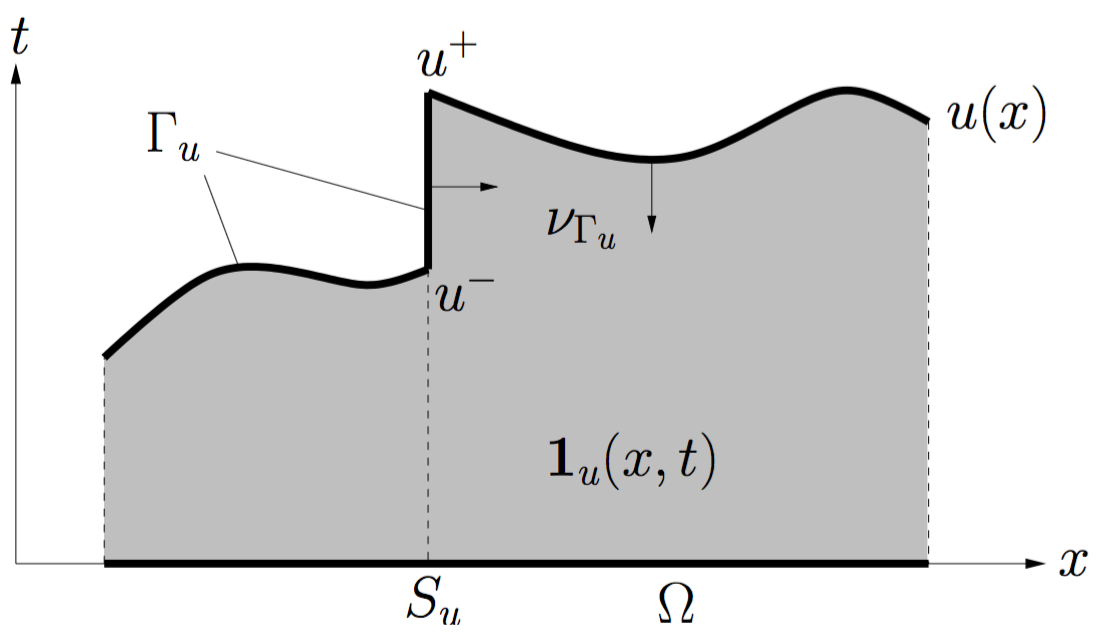
\includegraphics[width=0.8\textwidth]{img/char_func.png}
        \caption{This picture (found in \cite{Pock-et-al-iccv09}) shows the characteristic function of another function $u(x)$. The gray shaded area shows where $\mathds{1}_{u}(x, t) = 1$.}
        \label{fig:characteristic_function}
    \end{figure}

    \begin{remark}
        This lifiting method together with the following theorem assures, that the Mumford-Shah Model we are facing will be convex. As soon as we have a convex optimazation problem we can apply the primal-dual algorithm to solve it.
    \end{remark}

    Using this characteristic function, one can find in a series of paper (\cite{kelvey-sscv}, \cite{Alberti-et-al-cvpde}) a result of the convex relaxed Mumford-Shah Functional along with a proof of this result.

    \begin{theorem}[Convex Relaxation of the Mumford-Shah Functional]
    \label{convex_relaxation_of_the_mumford_shah_functional}
        For a function $u \in SBV(\Omega)$ the Mumford Shah functional can be written as
            \begin{equation}
                E(u) = \sup_{\varphi \in K} \int_{\Omega \times \mathbb{R}} \varphi D\mathds{1}_{u}, \label{eq:convex_relaxed_ms}
            \end{equation}
        with a convex set
            \begin{eqnarray}
                K = \bigg\{ \varphi \in C^{0}(\Omega \times \mathbb{R}, \mathbb{R}^{2}) &:& \varphi^{t}(x, t) \ge \frac{\varphi^{x}(x,t)^{2}}{4} - \lambda(t - f(x))^{2}, \\
                &&\bigg| \int^{t_{2}}_{t_{1}} \varphi^{x}(x,s)ds \bigg| \le \nu \bigg\}, \label{eq:set_k_continuous}
            \end{eqnarray}
        where the inequalities in the definition of $K$ hold for all $x \in \Omega$ and for all $t, t_{1}, t_{2} \in \mathbb{R}$.
    \end{theorem}

    \begin{remark}
        We used in the theorem, that we will represent a vector $\varphi \in K \subseteq \mathbb{R}^{n}$ by $\varphi(x, t) = \big( \varphi^{x}, \varphi^{t} \big)^{T}$, where $\varphi(x,t) \in \mathbb{R}^{n}$, $\varphi^{x} \in \mathbb{R}^{n-1}$ and $\varphi^{t} \in \mathbb{R}$.
    \end{remark}

    Our goal is now to minimize \ref{eq:convex_relaxed_ms} since minimizing the energy of this functional should lead to an optimal approximation $u$ of an input image $f$. Mathematically we have:

    \begin{equation}
        \min_{u \in X} E(u) = \min_{u \in X} \left( \sup_{\varphi \in K} \int_{\Omega \times \mathbb{R}} \varphi D\mathds{1}_{u} \right) \label{eq:minimize_convex_relaxed_ms}
    \end{equation}

    To compute the minimizer of this formulation we first want to substitute $\mathds{1}_{u}$ by a generic function
        \begin{equation}
            v(x, t): \Omega \times \mathbb{R} \longrightarrow [0, 1] \,\, \textnormal{which satisfies} \,\, \lim_{t \rightarrow -\infty} v(x, t) = 1, \, \, \, \lim_{t \rightarrow +\infty} v(x, t) = 0.
        \label{eq:generic_functions}
        \end{equation}
    This substitution is important to take into account, that we assume an image $u$ to be in $[0, 1]$ in this chapter. Unfortunatelly, this makes the proposed method inexact. But still, we are computing a lower bound to the global optimal solution. Further, if we only consider the characteristic function then one can show that for binary images the lower bound is indeed the global optimal value of \ref{eq:minimize_convex_relaxed_ms}. Overall, we are going to face the following, continous, convex optimization problem:
        \begin{equation}
            \min_{v \in [0, 1]} \sup_{\varphi \in K} \langle v, D\varphi \rangle = \min_{v \in [0, 1]} \sup_{\varphi \in K} \int_{\Omega \times \mathbb{R}} \varphi Dv. \label{eq:continous_saddle_point_problem}
        \end{equation}

    In the next section we will reformulate this minimization problem in the discrete setting. Additionally, we will formulate this section in the sense of the saddle-point problem \ref{eq:the_saddle_point_problem}.

% section convex_relaxation (end)

%     \section{Clarification} % (fold)
%     \label{sec:clarification}
        
%     % section clarification (end)

%     \section{A proof of convergence} % (fold)
%     \label{sec:a_proof_of_convergence}
        
%     % section a_proof_of_convergence (end)

%     \section{Minimizing the Mumford-Shah Functional} % (fold)
%     \label{sec:minimizing_the_mumford_shah_functional}
    
%     % section minimizing_the_mumford_shah_functional (end)

%         \section{Projection onto the convex sets and Dykstra's projection algorithm}

%             \subsection{Dykstra's projection algorithm} % (fold)
%             \label{sub:dykstra_s_projection_algorithm}
% %             Dykstra's algorithm finds for each r the only  \bar{x} \in C\cap D such that:

% %  \|\bar{x}-r\|^2\le \|x-r\|^2, \text{for all } x\in C \cap D, 
% % where C,D are convex sets. This problem is equivalent to finding the projection of r onto the set C\cap D, which we denote by \mathcal{P}_{C \cap D}.

%                 Consider $P$ \underline{convex} sets with $\mathbb{R}^{n} \ni X = X_{1} \cap X_{2} \cap ... \cap X_{P}$. Let $\Pi_{i}$ denote the projection onto the i-th set for $i = 1, ..., P$. And let $u_{c} \in \mathbb{R}^{n}$ be the current estimate with $u_{c} \notin X$, $u_{i}^{k} \in \mathbb{R}^{n}$ for $i = 0, ..., P$ and $v_{i}^{k} \in \mathbb{R}^{n}$ for $i = 1, ..., P$ and $k = 1, 2, ...$, where $k$ denotes the number of iterations. Then the algorithm of (Boyle and) Dykstra finds for a point $u_{c} \in \mathbb{R}^{n}$ the (only) $u^{\ast} \in X$ such that

%                 $$
%                     ||u^{\ast} - u_{c}||^{2} \le ||u - u_{c}||^{2} \,\,\, \forall u \in X.
%                 $$

%                 \begin{algorithm}\label{alg:dykstra}
%                     For $k = 1, 2, ...$ set $u^{0}_{P} = u_{c}$ and $v^{0}_{i} = 0$ for all $i = 1, ..., P$. Then iterate until convergence (e.g. $||u_{0}^{k} - u_{P}^{k}||_{2} \le \varepsilon$ with $\varepsilon$ small):

%                     \begin{eqnarray}
%                         &u_{0}^{k} = &u_{P}^{k-1}, \notag \\
%                         &\textnormal{for} \,\, &i = 1, 2, ..., P: \notag \\
%                         &&u_{i}^{k} = \Pi_{i}(u_{i-1}^{k} - v_{i}^{k-1}), \notag \\
%                         &&v_{i}^{k} = u_{i}^{k} - (u_{i-1}^{k} - v_{i}^{k-1}). \notag
%                     \end{eqnarray}
%                 \end{algorithm}

%                 \begin{proposition}
%                     The sequence $u_{0}^{k}$ in algorithm \ref{alg:dykstra} converges to the (only) point $u \in X$.
%                 \end{proposition}

%                 \begin{proof}
%                     For the proof, we refer to \cite{dykstra-et-al-aors14}.
%                     \qed
%                 \end{proof}
%             % section dykstra_s_projection_algorithm (end)

%             \subsection{Projection onto $C$}

%             One possible projection in the algorithm of Dykstra is the one onto the convex set $C$.This can be efficiently computed. To project on the set $[0, 1]$ we can easily see that this is a $l_{\infty}([0, 1])$ projection, i.e. we have:

%             % \begin{algbox}
%                 \begin{algorithm}[Clipping]
%                     To project a vector $x \in \mathbb{R}^{P \times N \times M}$ on the set
%                         \begin{equation}
%                             C = \{ x \in X: x(i,j,k) \in [0,1], \,\, x(i, j, 1) = 1, \,\, x(i, j, M) = 0 \}, \label{eq:limits}
%                         \end{equation}
%                     we have pointwise
%                         \begin{equation}
%                             x^{n+1}_{i,j,k} = \min\{1, \max \{ 0, x^{n}_{i, j, k} \} \}
%                         \end{equation}
%                     for all $i = 1, ..., P, j = 1, ..., N, k = 1, ..., M$.
%                 \end{algorithm}
%             % \end{algbox}

%             \begin{proof}
%                 Let $x^{n}_{i, j, k} \notin C$. Then let
%                 \begin{enumerate}
%                     \item $x^{n}_{i,j,k} < 0$. We have
%                     $$
%                         \underbrace{\min\{1, \underbrace{\max \{ 0, x^{n}_{i, j, k} \}}_{= 0} \}}_{= 0} \in [0, 1].
%                     $$
%                     \item $x^{n}_{i,j,k} > 1$. We have
%                     $$
%                         \underbrace{\min\{1, \underbrace{\max \{ 0, x^{n}_{i, j, k} \}}_{= x^{n}_{i, j, k}} \}}_{= 1} \in [0, 1].
%                     $$
%                 \end{enumerate}
%                 \qed
%             \end{proof}

%             % \begin{rebox}
%                 \begin{remark}
%                     By projecting onto $C$ we also need to take care about the limits in \ref{eq:limits}. For that we set $x(i, j, 1) = 1$ and $x(i, j, M) = 0$ in each projection.
%                 \end{remark}
%             % \end{rebox}

%             The projection onto the convex set $K$ is more involved since it takes into account local and non-local constraints. Therefore let us decompose the set into the sets

%             \begin{eqnarray}
%                 &K_{p}& = \bigg\{ y^{3}(i,j,k) \ge \frac{y^{1}(i,j,k)^{2} + y^{2}(i,j,k)^{2}}{4} - \lambda(\frac{k}{M} - f(i,j))^{2} \bigg\} \,\,\, \forall i, j, k \notag \\
%                 \Longleftrightarrow &K_{p}& = \bigg\{ y^{t}(i, j, k) \ge \frac{||y^{x}(i, j, k)||^{2}}{4} - \lambda(\frac{k}{M} - f(i,j))^{2} \bigg\} \,\,\, \forall i, j, k \label{eq:parabola}
%             \end{eqnarray}

%             where $y^{t}(i, j, k) = y^{3}(i, j, k)$ and $y^{x}(i, j, k) := (y^{1}(i, j, k), y^{2}(i, j, k))^{T}$. For the non-local constraint we have

%             \begin{equation}
%                 K_{nl} = \bigg\{ \left| \sum_{k_{1} \le k \le k_{2}} (y^{1}(i,j,k), y^{2}(i,j,k))^{T} \right| \le \nu \bigg\} \,\,\, \forall i, j, k_{1} \le k \le k_{2} \label{eq:nonlocal}
%             \end{equation}

%             being the non-local constraint. Then we have $K = K_{p} \cap K_{nl}$. Since $K_{p}$ is an intersection of $P \cdot N \cdot M$ set and $K_{nl}$ is an intersection of $P \cdot N \cdot (\frac{M(M-1)}{2} + M)$ sets we need an algorithm which can handle the projection of a point onto (convex) sets. First let us introduce the projections onto $K_{p}$ and $K_{nl}$.

%             \subsection{Projection onto $K_{p}$}

%                 % Since the projection onto this set also goes pointwise, we have several possibilities to compute the orthogonal projection onto a parabola.\\
%                 Since the projection onto the set $K_{p}$ is pointwise we want to drop the indices $(i, j, k)$. Note that we do not necessarily need that a $y^{x}$ is an element of $\mathbb{R}^{2}$. The following derivation holds for a larger class of problems namely having $y^{x} \in \mathbb{R}^{n}$.
%                 % To understand how a projection on a parabola can be computed we want to reformulate \ref{eq:localconst} into an optimization problem.\\
%                 \begin{describe}[]
%                     Let $\alpha > 0$, $y^{x} \in \mathbb{R}^{n}$, $y^{t} \in \mathbb{R}$ %(in our case we would have
%                     %$$
%                      %   y^{t} := y^{3}(i, j, k) + \lambda \bigg( \frac{k}{M} - f(i, j)\bigg)^{2}
%                     %$$
%                     %for all $i = 1, ..., P$, $j = 1, ..., N$, $k = 1, ..., M$) and
%                     $y = (y^{x}, y^{t})^{T} \in \mathbb{R}^{n} \times \mathbb{R}$.
%                     The projection of a $y_{0}$ with $y_{0}^{t} < \alpha ||y_{0}^{x}||_{2}^{2}$ can be written as

%                     \begin{eqnarray}
%                         &\min\limits_{y \in \mathbb{R}^{n} \times \mathbb{R}}& \frac{1}{2} ||y - y_{0}||_{2}^{2} \notag \\
%                         &\textnormal{subject to}& y^{t} \ge \alpha||y^{x}||_{2}^{2} \notag
%                     \end{eqnarray}

%                     An equivalent notation for this problem is

%                     \begin{eqnarray}
%                         &\min\limits_{y \in \mathbb{R}^{n} \times \mathbb{R}}& f(y) := \frac{(y - y_{0})^{2}}{2} \notag \\
%                         &\textnormal{subject to}& g(y) := y^{t} - \alpha ||y^{x}||_{2}^{2} \ge 0 \notag
%                     \end{eqnarray}
%                 \end{describe}

%                 To find the solution of this optimization problem we introduce some auxiliary variable (or Lagrange Multiplier) $\mu \in \mathbb{R}$ and define the Lagrangian as

%                 \begin{equation}
%                     \mathcal{L}(x, y, \mu) = f(y) - \mu g(y) = \frac{(y - y_{0})^{2}}{2} - \mu \bigg( y^{t} - \alpha||y^{x}||_{2}^{2} \bigg).
%                 \end{equation}

%                 Seeking for the local minima where $\nabla \mathcal{L}(x, y, \mu) = 0$ we even get a global minimum since our function to optimize is convex, the inequality constraint is convex and the feasible set $\mathbb{R}^{n} \times \mathbb{R}$ is also convex. We set

%                 \begin{equation}
%                     \nabla \mathcal{L}(y, \mu) =
%                     \begin{pmatrix}
%                         \partial_{y^{x}} \mathcal{L}(y, \mu) \\
%                         \partial_{y^{t}} \mathcal{L}(y, \mu) \\
%                         \partial_{\mu} \mathcal{L}(y, \mu)
%                     \end{pmatrix} = 
%                     \begin{pmatrix}
%                         y^{x} - y_{0}^{x} - \mu 2 \alpha y^{x} \\
%                         y^{t} - y_{0}^{t} - \mu \\
%                         y^{t} - \alpha||y^{x}||_{2}^{2}
%                     \end{pmatrix}
%                     = 0. \label{eq:linearSystem}
%                 \end{equation}

%                 That means, we need to solve a linear system. The first equation gives us

%                 \begin{equation}
%                     y_{0}^{x} = (\mu 2 \alpha + 1) y^{x} \Longleftrightarrow y^{x} = \frac{y_{0}^{x}}{\mu 2 \alpha + 1}, \label{eq:1stequ}
%                 \end{equation}

%                 and the second equation leads us to

%                 \begin{equation}
%                     y^{t} = y_{0}^{t} + \mu. \label{eq:2ndequ}
%                 \end{equation}

%                 At this point we can solve this system in two ways - if $y_{0}^{t} \ge \alpha ||y_{0}^{x}||_{2}^{2}$ is not true already
%                 \begin{enumerate}
%                     \item By plugging these two equalities into the third equation, we get

%                 \begin{eqnarray}
%                     y_{0}^{t} + \mu - \alpha \bigg|\bigg|\frac{y_{0}^{x}}{\mu 2 \alpha + 1}\bigg|\bigg|_{2}^{2} = 0 &\Longleftrightarrow& y_{0}^{t} + \mu - \frac{\alpha}{(\mu 2 \alpha + 1)^{2}} ||y_{0}^{x}||_{2}^{2} = 0 \notag \\
%                     &\Longleftrightarrow& (\mu 2 \alpha + 1)^{2} y_{0}^{t} + (\mu 2 \alpha + 1)^{2} \mu - \alpha ||y_{0}^{x}||_{2}^{2} = 0 \notag \\
%                     &\Longleftrightarrow& (4 \mu^{2} \alpha^{2} + 4 \mu \alpha + 1) y_{0}^{t} + 4 \mu^{3} \alpha^{2} + 4 \mu^{2} \alpha + \mu - \alpha ||y_{0}^{x}||_{2}^{2} = 0 \notag \\
%                     &\Longleftrightarrow& 4 \alpha^{2} \mu^{3} + \mu^{2} (4 \alpha^{2} y_{0}^{t} + 4 \alpha) + \mu (4 \alpha y_{0}^{t} + 1) + y_{0}^{t} - \alpha ||y_{0}^{x}||_{2}^{2} = 0. \notag
%                 \end{eqnarray}

%                 Solving this equation is straightforward since computing the zeroes can be done by Newton's algorithm with

%                 \begin{equation}
%                     \mu^{k+1} = \mu^{k} - \frac{h(\mu)}{h^{'}(\mu)}, \label{eq:newton}
%                 \end{equation}

%                 for $k = 1, 2, ...$.

%                 If we set
%                 $$
%                     h(\mu) = 4 \alpha^{2} \mu^{3} + \mu^{2} (4 \alpha^{2} y_{0}^{t} + 4 \alpha) + \mu(4 \alpha y_{0}^{t} + 1) + y_{0}^{t} - \alpha ||y_{0}^{x}||_{2}^{2},
%                 $$
%                 we observe
%                 $$
%                     h^{'}(\mu) = 12 \alpha^{2} \mu^{2} + 2 \mu (4 \alpha^{2} y_{0}^{t} + 4 \alpha) + (4 \alpha y_{0}^{t} + 1).
%                 $$
%                 At the end we are having the update of a $\mu^{k+1}$ with
%                 \begin{equation}
%                     \mu^{k+1} = \mu^{k} - \frac{4 \alpha^{2} \mu^{3} + \mu^{2} (4 \alpha^{2} y_{0}^{t} + 4 \alpha) + \mu(4 \alpha y_{0}^{t} + 1) + y_{0}^{t} - \alpha ||y_{0}^{x}||_{2}^{2}}{12 \alpha^{2} \mu^{2} + 2 \mu (4 \alpha^{2} y_{0}^{t} + 4 \alpha) + (4 \alpha y_{0}^{t} + 1)}.
%                 \end{equation}
%                 In \cite{Chambolle-et-al-10} they suggest setting $\mu^{0} = \max \{ 0, - \frac{2 y_{0}^{t}}{3} \}$. The algorithm converges within 10-20 iterations to a quite accurate solution.\\
%                 The projected vector $y$ of our problem is then given by
%                 \begin{equation}
%                     y = \bigg( \frac{y_{0}^{x}}{\mu 2 \alpha + 1}, y_{0}^{t} + \mu \bigg). \label{eq:newtonSolution}
%                 \end{equation}

%                 \item For the second approach we note that \ref{eq:1stequ} and \ref{eq:2ndequ} hold and the third equation in \ref{eq:linearSystem} can only hold if
%                 \begin{equation}
%                     y^{t} = \alpha ||y^{x}||_{2}^{2} \Longleftrightarrow \alpha ||y^{x}||_{2}^{2} = y_{0}^{t} + \mu. \label{eq:tmp1}
%                 \end{equation}
%                 With \ref{eq:1stequ} we can also compute the solution of $\mu$ by noticing that

%                 \begin{eqnarray}
%                     ||y^{x}||_{2} = \bigg|\bigg| \frac{y_{0}^{x}}{1 + 2 \alpha \mu} \bigg|\bigg|_{2} &\Longleftrightarrow& ||y^{x}||_{2} = \frac{1}{1 + 2 \alpha \mu} ||y_{0}^{x}||_{2} \notag \\
%                     &\Longleftrightarrow& \frac{1}{1 + 2 \alpha \mu} = \frac{||y^{x}||_{2}}{||y_{0}^{x}||_{2}} \notag \\
%                     &\Longleftrightarrow& 2 \alpha \mu = \frac{||y_{0}^{x}||_{2}}{||y^{x}||_{2}} - 1 \notag \\
%                     &\Longleftrightarrow& \mu = \frac{1}{2 \alpha} \bigg( \frac{||y_{0}^{x}||_{2}}{||y^{x}||_{2}} \bigg). \notag
%                 \end{eqnarray}

%                 Using the solution of $\mu$ in \ref{eq:tmp1} we get

%                 \begin{eqnarray}
%                     \alpha ||y^{x}||_{2}^{2} = y_{0}^{t} + \frac{1}{2 \alpha} \bigg( \frac{||y_{0}^{x}||_{2}}{||y^{x}||_{2}} \bigg) &\overbrace{\Longleftrightarrow}^{\cdot 2 \alpha ||y^{x}||_{2}}& 2 \alpha^{2} ||y^{x}||_{2}^{3} = 2 \alpha ||y^{x}||_{2} y_{0}^{t} + ||y_{0}^{x}||_{2} - 1 \notag \\
%                     &\Longleftrightarrow& 2 \alpha^{2} ||y^{x}||_{2}^{3} + (1 - 2 \alpha y_{0}^{t}) ||y^{x}||_{2} - ||y_{0}^{x}||_{2} = 0. \notag \\ 
%                     &\overbrace{\Longleftrightarrow}^{\cdot 4 \alpha}& 8 \alpha^{3} ||y^{x}||_{2}^{3} + 4 \alpha (1 - 2 \alpha y_{0}^{t}) ||y^{x}||_{2} - 4 \alpha ||y_{0}^{x}||_{2} = 0. \notag \\
%                     &\Longleftrightarrow& (2 \alpha ||y^{x}||_{2})^{3} + 2 (1 - 2 \alpha y_{0}^{t}) 2 \alpha ||y^{x}||_{2} - 4 \alpha ||y_{0}^{x}||_{2} = 0. \notag \\
%                     &\Longleftrightarrow& t^{3} + 3bt - 2a = 0, \label{eq:cubic}
%                 \end{eqnarray}

%                 with $a = 2 \alpha ||y_{0}^{x}||_{2}$, $b = \frac{2}{3}(1 - 2 \alpha y_{0}^{t})$ and $t = 2 \alpha ||y^{x}||_{2}$.\\
%                 The cubic equation \ref{eq:cubic} in $t$ can efficiently be solved using \cite{kelvey-ajp}.

%                 \end{enumerate}

%                 The result of the work mentioned is summarized in the following algorithm. Notice that we already computed the factors $a$ and $b$. The others follow through the proof.

%                 % After computing the optimal $\mu$ we get the solution to our optimization problem by plugging the Lagrange Multiplier into \ref{eq:1stequ} and \ref{eq:2ndequ} and computing $y^{x}, y^{t}$ respectively.

%                 % \begin{enumerate}
%                 %     \item Using Lagrange-Multipliers to rewrite the minimization problem and then applying Newton's method.
%                 %     \item Following a straightforward formulation proposed in (Evgeny).
%                 % \end{enumerate}

%                 % We want to start with the method proposed in (Evgeny).

%                     \begin{algorithm}
%                         % Let $\alpha > 0$. For $y_{0}^{x} \in \mathbb{R}^{n}$ and $y_{0} \in \mathbb{R}$ the projection onto the parabola of the form

%                         % \begin{equation}
%                         %     \arg \min_{x \in \mathbb{R}^{n}, y \in \mathbb{R}, y \ge \alpha ||x||_{2}^{2}} \frac{(x - y_{0}^{x})^{2}}{2} + \frac{(y - y_{0})^{2}}{2}.
%                         % \end{equation}

%                         If already $y_{0}^{t} \ge \alpha ||y_{0}^{x}||_{2}^{2}$, the solution is $(y^{x}, y^{t}) = (y_{0}^{x}, y_{0}^{t})$. Otherwise, with $a := 2 \alpha ||y_{0}^{x}||_{2}$, $b := \frac{2}{3} (1 - 2 \alpha y_{0}^{t})$, and

%                             \[
%                                 d =
%                                     \begin{dcases*}
%                                         a^{2} + b^{3} & \textnormal{if $b \ge 0$}\\
%                                         (a - \sqrt{-b}^{3})(a + \sqrt{-b}^{3}) & \textnormal{else}
%                                     \end{dcases*}
%                             \]

%                         set

%                             \[
%                                 v =
%                                     \begin{dcases*}
%                                         c - \frac{b}{c} \,\, \textnormal{with} \,\, c = \sqrt[3]{a + \sqrt{d}} & \textnormal{if $d \ge 0$}\\
%                                         2 \sqrt{-b} \cos \bigg( \frac{1}{3} \arccos \frac{a}{\sqrt{-b}^{3}} \bigg) & \textnormal{else}.
%                                     \end{dcases*}
%                             \]

%                         If $c = 0$ in the first case, set $v := 0$. The solution is then given by

%                             \[
%                                 y^{x} =
%                                     \begin{dcases*}
%                                         \frac{v}{2\alpha} \frac{y_{0}^{x}}{||y_{0}^{x}||_{2}} & \textnormal{if $y_{0}^{x} \ne 0$}\\
%                                         0 & \textnormal{else}
%                                     \end{dcases*}
%                             \]

%                         and $y^{t} = \alpha ||y^{x}||_{2}^{2}$.
%                     \end{algorithm}

%                     % \begin{proof}
%                     %     Later...
%                     % \end{proof}

%                 The above method states that the projection onto the parabola can be done by one cycle of straightforward computations. The implementation of it is quite simple and computation time is fast.% But as mentioned there is another approach for this projection.\\

%             \subsection{Projection onto $K_{nl}$}

%                 This set is a combination of non-local constraints, meaning that in a fixed point $(i, j, k)$ you sum up for all $k_{1} \le k \le k_{2}$. For that reason you can not project pointwise. First of all we want to present the algorithm:

%                 % Let $y_{k} := (y^{1}(i, j, k), y^{2}(i, j, k))^{T}$. Then the projection $y = (y_{1}, ..., y_{M})^{T}$ of a $y_{0} = (y_{0}_{1}, ..., y_{0}_{M})^{T}$ is - for each combination $k_{1} \le k \le k_{2}$ - of the following problem:
%                 % \begin{algbox}
%                     \begin{algorithm}[Soft Shrinkage Scheme]\label{alg:softshrinkage}
%                         Let $y^{i}_{k} := (y^{1}(i, j, k), y^{2}(i, j, k))^{T} \in \mathbb{R}^{2}$, $y^{i} := (y^{i}_{1}, ..., y^{i}_{M})^{T} \in \mathbb{R}^{2 \times M}$ for all $i = 1, 2, ...$. Then the projection $y^{n+1}$ of a $y^{n}$ - for an arbitrary, fixed pair $(k_{1}, k_{2})$ with $1 \le k_{1} \le k \le k_{2} \le M$ - is computed by:

%                             \[
%                                 y^{n+1} =
%                                     \begin{dcases*}
%                                         y^{n} + \frac{s - \tilde{s}}{k_{2} - k_{1} + 1} & \textnormal{if $k_{1} \le k \le k_{2}$}, \\
%                                         y^{n} & \textnormal{else},
%                                     \end{dcases*}
%                             \]

%                         where $s \in \mathbb{R}^{2}, \tilde{s} \in \mathbb{R}^{2}$ with

%                             $$\tilde{s} = \sum_{k_{1} \le k \le k_{2}} y_{k}$$

%                         and

%                             \[
%                                 s =
%                                     \begin{dcases*}
%                                         \tilde{s} & \textnormal{if $||\tilde{s}||_{2} \le \nu$},\\
%                                         \Pi_{||\cdot||_{2} \le \nu}(\tilde{s}) = \frac{\nu}{||\tilde{s}||_{2}} \tilde{s} & \textnormal{else}.
%                                     \end{dcases*}
%                             \]

%                         % \begin{equation}
%                         %     \min\limits_{y_{k} \in \mathbb{R}^{2}} \frac{1}{2} \sum_{k = 1}^{M} ||y_{k} - \tilde{y}_{k}||^{2} \,\,\, \textnormal{s.t.} \,\,\, \bigg{|} \bigg{|} \sum_{k_{1} \le k \le k_{2}} (y^{1}(i, j, k), y^{2}(i, j, k))^{T} \bigg{|} \bigg{|}_{2} \le \nu. \label{eq:minnonlocal}
%                         % \end{equation}
%                         % It follows that we have $y_{k} = \tilde{y}_{k}$ for all $k < k_{1}$ and $k > k_{2}$.\\
%                         % If $k_{1} \le k \le k_{2}$ one can show that we have:
%                         % \begin{equation}
%                         %     y_{k} = \tilde{y}_{k} + \frac{s - s_{0}}{k_{2} - k_{1} + 1},
%                         % \end{equation}
%                         % where
%                         % $$s_{0} = \sum_{k_{1} \le k \le k_{2}} \tilde{y}_{k}$$
%                         % and
%                         % $$s = \Pi_{||\cdot||_{l^{2}} \le \nu} (s_{0}).$$
%                     \end{algorithm}
%                 % \end{algbox}

%                 Since this procedure needs a clarification, we want to introduce the KKT conditions.

%                 % \begin{defbox}
%                     \begin{theorem}[Karush-Kuhn-Tucker Optimality Conditions]
%                         Consider the optimization problem
%                         \begin{eqnarray}
%                             \min_{x \in \mathbb{R}^{n}} &&f(x) \notag \\
%                             \textnormal{s.t.} \,\, && g_{i}(x) \le 0, i = 1, ..., m \notag
%                         \end{eqnarray}

%                         Defining the Lagrangian function to this optimization problem we have

%                         \begin{equation}
%                             \mathcal{L}(x, \lambda) = f(x) + \lambda, g(x),
%                         \end{equation}

%                         with $\lambda \in \mathbb{R}^{m}$ are called the Lagrange-Multipliers.\\

%                         Then if the objective function $f: \mathbb{R}^{n} \longrightarrow \mathbb{R}$ and the constraint functions $g_{i}: \mathbb{R} \longrightarrow \mathbb{R}$ are continously differentiable at a point $x^{*}$ then it holds:\\
%                         $$x^{*} \, \textnormal{is a local minimum} \, \Longleftrightarrow \, \textnormal{there exists a unique} \, \lambda^{*} \, \textnormal{such that}$$
%                         \begin{itemize}
%                             \item Stationarity:
%                             $$\nabla_{x} \mathcal{L}(x^{*}, \lambda^{*}) = 0$$
%                             \item Complementary Slackness:
%                             $$\lambda^{*}_{i} g(x^{*}) = 0 \, \, \, \forall i = 1, ..., m$$
%                             \item Primal Feasibility:
%                             $$g_{i}(x^{*}) \le 0 \, \, \, \forall i = 1, ..., m$$
%                             \item Dual Feasibility:
%                             $$\lambda^{*}_{i} \ge 0 \, \, \, \forall i = 1, ..., m$$
%                         \end{itemize}
%                     \end{theorem}
%                 % \end{defbox}

%             \begin{proof}[Proof of Algorithm \ref{alg:softshrinkage}]
%                 Let $y_{k}, \tilde{y}_{k} \in \mathbb{R}^{2}$ and $y, \tilde{y} \in \mathbb{R}^{2 \times M}$ have the same form as in \ref{alg:softshrinkage}. Then for a fixed pair $(k_{1}, k_{2})$ we face the following optimization problem: %$K = k_{2} - k_{1} + 1$, $m = \frac{M(M-1)}{2}$, 
%                 % $y_{k} \in \mathbb{R}^{2}$, $\tilde{y}_{k} \in \mathbb{R}^{2}$, $y = (y_{1}, ..., y_{M})^{T} \in \mathbb{R}^{2 \times M}$ and $\tilde{y} = (\tilde{y}_{1}, ..., \tilde{y}_{M})^{T} \in \mathbb{R}^{2 \times M}$. Then for a fixed pair $(k_{1}, k_{2})$ we have% have that \ref{eq:minnonlocal} is equivalent to

%                 \begin{eqnarray}
%                     &\min\limits_{y \in \mathbb{R}^{2 \times M}}& \frac{1}{2} ||y - \tilde{y}||^{2}_{2} \notag \\
%                     &\textnormal{subject to}& \bigg{|} \bigg{|} \sum_{k_{1} \le k \le k_{2}} y_{k} \bigg{|} \bigg{|}_{2} \le \nu. \notag
%                 \end{eqnarray}

%                 This equivalent to

%                 \begin{eqnarray}
%                     &\min\limits_{y \in \mathbb{R}^{2 \times M}}& f(y) \notag \\
%                     &\textnormal{subject to}& g(y) \le 0, \label{eq:inequalityConstraint}
%                 \end{eqnarray}

%                 if we set
%                     $$f(y) = \sum_{k = 1}^{M} \frac{(y_{k} - \tilde{y}_{k})^{2}}{2}$$
%                 and
%                     $$g(y) = \frac{1}{2} \bigg{|} \bigg{|} \sum_{k_{1} \le k \le k_{2}} y_{k} \bigg{|} \bigg{|}_{2}^{2} - \frac{1}{2} \nu^{2}.$$

%                 This problem states that we try to find the closest $y$ to $\tilde{y}$ whose components fullfil the inequality constraint in \ref{eq:inequalityConstraint}.\\

%                 % \begin{equation}
%                 %     \min\limits_{y_{k} \in \mathbb{R}^{2}} \frac{1}{2} \sum_{k = 1}^{M} ||y_{k} - \tilde{y}_{k}||^{2} \,\,\, \textnormal{s.t.} \,\,\, \frac{1}{2} \bigg{|} \bigg{|} \sum_{k_{1} \le k \le k_{2}} (y^{1}(i, j, k), y^{2}(i, j, k))^{T} \bigg{|} \bigg{|}_{2}^{2} - \frac{1}{2} \nu^{2} \le 0 \notag
%                 % \end{equation}

%                 Let us now introduce a new variable $\lambda \in \mathbb{R}$ which is called Lagrange Multiplier and observe the Lagrange function (or Lagrangian) with

%                 % \begin{equation}
%                 %     \min_{y \in \mathbb{R}^{2 \times M}} f(y) \,\,\, \textnormal{s.t.} \,\,\, g_{i}(y) \le \nu \,\,\, \forall i = 1, ..., m \notag
%                 % \end{equation}

%                 % has the following form

%                 \begin{equation}
%                     \mathcal{L}(y, \lambda) = f(y) + \lambda g(y)% = \frac{1}{2} \sum_{k = 1}^{M} ||y_{k} - \tilde{y}_{k}||^{2} + \sum_{l = 1}^{K} \lambda_{l} g_{l}(y),
%                 \end{equation}

%                 Looking at \underline{Stationarity} condition to find a valid $\lambda^{\ast}$ and $y^{\ast}$ leads us to:

%                 \begin{equation}
%                     \nabla_{y} \mathcal{L}(y^{\ast}, \lambda^{\ast}) = \nabla_{y} f(y^{\ast}) + \lambda \nabla_{y} g(y^{\ast}) =
%                     \underbrace{\begin{pmatrix}
%                         y^{\ast}_{1} - \tilde{y}_{1} \\
%                          \\
%                         \vdots \\
%                          \\
%                         y^{\ast}_{M} - \tilde{y}_{M}
%                     \end{pmatrix}}_{\in \mathbb{R}^{M}}
%                     + \lambda^{\ast}
%                     \underbrace{\begin{pmatrix}
%                         0 \\
%                         \vdots \\
%                         0 \\
%                         \sum\limits_{k_{1} \le k \le k_{2}} y^{\ast}_{k} \\
%                         \vdots \\
%                         \sum\limits_{k_{1} \le k \le k_{2}} y^{\ast}_{k} \\
%                         0 \\
%                         \vdots \\
%                         0
%                     \end{pmatrix}}_{\in \mathbb{R}^{M}}
%                     = 0,
%                 \end{equation}

%                 where the zeroes in the last vector are obtain for all components where $k < k_{1}$ and $k > k_{2}$. In these lines we already see that we get

%                     $$y^{\ast}_{k} = \tilde{y}_{k} \,\,\, \textnormal{if} \,\, k < k_{1} \,\, \textnormal{and} \,\, k > k_{2}.$$

%                 Let us now take a closer look at the i-th line where $\nabla_{y_{k}} g(y) \ne 0$. Then we have

%                     \begin{equation}
%                         y^{\ast}_{i} - \tilde{y}_{i} + \lambda^{\ast} \sum_{k_{1} \le k \le k_{2}} y^{\ast}_{k} = 0. \label{eq:ithRow}
%                     \end{equation}

%                 We set % state that the optimal $\lambda^{\ast}$ is of the form

%                 %     \begin{equation}
%                 %         \lambda^{\ast} = \frac{1}{k_{2} - k_{1} + 1} \bigg( \frac{\nu}{||\tilde{s}||_{2}} - 1 \bigg). \label{eq:lambda}
%                 %         % \lambda^{\ast} = \frac{\nu}{||\sum\limits_{k_{1} \le k \le k_{2}} y^{\ast}||_{2}} - 1. \label{eq:lambda}
%                 %     \end{equation}

%                 % with

%                     $$\tilde{s} := \sum\limits_{k_{1} \le k \le k_{2}} \tilde{y}_{k}$$

%                 and define a $s \in \mathbb{R}^{2}$ as

%                     \[
%                         s =
%                             \begin{dcases*}
%                                 \tilde{s} & \textnormal{if $||\tilde{s}||_{2} \le \nu$},\\
%                                 \Pi_{||\cdot||_{2} \le \nu}(\tilde{s}) = \frac{\nu}{||\tilde{s}||_{2}} \tilde{s} & \textnormal{else}.
%                             \end{dcases*}
%                     \]

%                 \newpage

%                 For finding the optimal values $y^{\ast}_{k}$ we want to distinguish between two cases:

%                 \begin{enumerate}
%                     \item $||\sum\limits_{k_{1} \le k \le k_{2}} \tilde{y}_{k}||_{2} \le \nu$:\\
%                     Setting $y^{\ast}_{k} = \tilde{y}_{k} + \frac{s - \tilde{s}}{k_{2} - k_{1} + 1} = \tilde{y}_{k}$ for all $k_{1} \le k \le k_{2}$ and $s = \tilde{s}$ leads to
%                         \begin{equation}
%                             \frac{1}{2} ||\sum_{k_{1} \le k \le k_{2}} y^{\ast}_{k}||_{2}^{2} - \frac{1}{2} \nu^{2} \le 0, \label{eq:caseOne}
%                         \end{equation}
%                     % which validates the \underline{Primal Feasibility} condition.
%                     It follows for the \underline{Complementary Slackness} condition that we can choose an arbitrary $\lambda^{\ast} \ge 0$ if we have equality in \ref{eq:caseOne} and $\lambda^{\ast} = 0$ else to derive the \underline{Dual Feasibility} condition. We set
%                     % The \underline{Complementary Slackness} condition claims that in this case% validates the \underline{Dual Feasibility} condition in this case because having equality in \ref{eq:caseOne} leads to
%                         $$\lambda^{\ast} = 0.$$

%                     % since $||\tilde{s}||_{2} \le \nu$.
%                     % which is equivalent to
%                         % ||\tilde{s}||_{2} = ||\sum\limits_{k_{1} \le k \le k_{2}} \tilde{y}^{k}||_{2} = 
%                         % $$\frac{\nu}{||\tilde{s}||_{2}} - 1 = 0 \Longleftrightarrow ||\tilde{s}||_{2} = \nu.$$
%                     % On the other hand if the inequality holds we have
%                     %     % ||\tilde{s}||_{2} = ||\sum\limits_{k_{1} \le k \le k_{2}} \tilde{y}^{k}||_{2} = 
%                     %     $$||\sum\limits_{k_{1} \le k \le k_{2}} y^{\ast}_{k}||_{2} < \nu \Longrightarrow \lambda^{\ast} = \underbrace{\frac{\nu}{||\sum\limits_{k_{1} \le k \le k_{2}} y^{\ast}_{k}||_{2}}}_{> 1} - 1 > 0.$$
%                     % Then $\lambda^{\ast}$ additionally satisfies the \underline{Complementary Slackness} condition.
%                     \item $||\sum\limits_{k_{1} \le k \le k_{2}} \tilde{y}_{k}||_{2} > \nu$:\\
%                     % If the equality holds we know that $s(\tilde{s})$
%                     Here, we would violate the \underline{Primal Feasibility} condition if we set $y^{\ast}_{k} = \tilde{y}_{k}$ for all $k_{1} \le k \le k_{2}$. For this reason we choose
%                         $$y^{\ast}_{k} = \tilde{y}_{k} + \frac{s - \tilde{s}}{k_{2} - k_{1} + 1} \,\,\,\,\,\, \forall k_{1} \le k \le k_{2}$$
%                         % $$y^{\ast}_{k} = \frac{\nu}{||\tilde{s}||_{2}} \tilde{y}_{k} \,\,\,\,\,\, \forall k_{1} \le k \le k_{2}$$
%                     We observe for the \underline{Primal Feasibility} condition that
%                         \begin{eqnarray}
%                             \frac{1}{2} ||\sum_{k_{1} \le k \le k_{2}} y^{\ast}_{k}||_{2}^{2} - \frac{1}{2} \nu^{2} &=& \label{eq:caseTwo} \\
%                             &=& \frac{1}{2(k_{2} - k_{1} + 1)} ||\sum_{k_{1} \le k \le k_{2}} \tilde{y}_{k} + (s - \tilde{s})||_{2}^{2} - \frac{1}{2} \nu^{2}\notag \\
%                             &=& \frac{1}{2} ||\sum_{k_{1} \le k \le k_{2}} \tilde{s} + s - \tilde{s}||_{2}^{2} - \frac{1}{2} \nu^{2} = \frac{1}{2} \underbrace{||s||_{2}^{2}}_{= \nu^{2}} - \frac{1}{2} \nu^{2} = 0. \notag
%                         \end{eqnarray}
%                     Using this equality we already see that \underline{Complementary Slackness} is fullfild with a \underline{dual feasible} $\lambda^{\ast} \ge 0$. Since we set $y^{\ast}_{k} = \tilde{y}_{k} + \frac{s - \tilde{s}}{k_{2} - k_{1} + 1}$ we can plug $y^{\ast}$ into \ref{eq:ithRow} to derive $\lambda^{\ast}$. It follows %We still need to proof that \ref{eq:lambda} is valid with this choice of $y^{\ast}_{k}$.

%                         \begin{eqnarray}
%                             &&y^{\ast}_{i} - \tilde{y}_{i} + \frac{\lambda^{\ast}}{k_{2} - k_{1} + 1} \sum_{k_{1} \le k \le k_{2}} y^{\ast}_{k} = \notag \\
%                             &=& \tilde{y}_{i} + \frac{s - \tilde{s}}{k_{2} - k_{1} + 1} - \tilde{y}_{i} + \frac{\lambda^{\ast}}{k_{2} - k_{1} + 1} \sum_{k_{1} \le k \le k_{2}} \tilde{y}_{k} + \frac{s - \tilde{s}}{k_{2} - k_{1} + 1} \notag \\
%                             &=& \frac{s - \tilde{s}}{k_{2} - k_{1} + 1} + \frac{\lambda^{\ast}}{k_{2} - k_{1} + 1} \bigg( \underbrace{\sum_{k_{1} \le k \le k_{2}} \tilde{y}_{k}}_{= \tilde{s}} + \underbrace{\sum_{k_{1} \le k \le k_{2}} \frac{s - \tilde{s}}{k_{2} - k_{1} + 1}}_{= \frac{(k_{2} - k_{1} + 1) (s - \tilde{s})}{k_{2} - k_{1} + 1} = s - \tilde{s}} \bigg) \notag \\
%                             &=& \frac{s - \tilde{s}}{k_{2} - k_{1} + 1} + \frac{\lambda^{\ast}}{k_{2} - k_{1} + 1} (\tilde{s} + s - \tilde{s}) \notag \\
%                             &=& \frac{s - \tilde{s}}{k_{2} - k_{1} + 1} + \frac{\lambda^{\ast}}{k_{2} - k_{1} + 1}s \notag \\
%                             &=& \frac{1}{k_{2} - k_{1} + 1} (s - \tilde{s} + \lambda^{\ast}s) = 0 \label{eq:equalsZero}
%                         \end{eqnarray}

%                     Now we can solve for $\lambda^{\ast}$ using that the last equation \ref{eq:equalsZero} is equivalent to

%                         \begin{eqnarray}
%                             (s - \tilde{s} + \lambda^{\ast} s) = 0 &\overbrace{\Longleftrightarrow}^{||\tilde{s}||_{2} > \nu}& \bigg(\frac{\nu}{||\tilde{s}||_{2}}\tilde{s} - \tilde{s} + \lambda^{\ast} \frac{\nu}{||\tilde{s}||_{2}}\tilde{s} \bigg) = 0 \notag \\
%                             &\Longleftrightarrow& \tilde{s} \bigg( \frac{\nu}{||\tilde{s}||_{2}} - 1 + \lambda^{\ast} \frac{\nu}{||\tilde{s}||_{2}} \bigg) = 0 \notag \\
%                             &\Longleftrightarrow& \frac{\nu}{||\tilde{s}||_{2}} - 1 + \lambda^{\ast} \frac{\nu}{||\tilde{s}||_{2}} = 0 \notag \\
%                             &\Longleftrightarrow& \lambda^{\ast} \frac{\nu}{||\tilde{s}||_{2}} = 1 - \frac{\nu}{||\tilde{s}||_{2}} \notag \\
%                             &\Longleftrightarrow& \lambda^{\ast} = \underbrace{\frac{||\tilde{s}||_{2}}{\nu}}_{> 1} - 1 > 0. \notag
%                         \end{eqnarray}

%                     This satisfies the \underline{Dual Feasibility} condition.

%                         % $$||\tilde{s}||_{2} = ||\sum\limits_{k_{1} \le k \le k_{2}} \tilde{y}_{k}||_{2} = ||\sum\limits_{k_{1} \le k \le k_{2}} \frac{||\tilde{s}||_{2}}{\nu} y^{\ast}||_{2} = ||\tilde{s}||_{2} =  \nu \Longrightarrow \lambda^{\ast} = 1 - 1 = 0.$$

%                         % $$\nu = ||\sum\limits_{k_{1} \le k \le k_{2}} y^{\ast}_{k}||_{2} = ||\frac{\nu}{||\tilde{s}||_{2}} \sum\limits_{k_{1} \le k \le k_{2}} \tilde{y}^{k}||_{2} = ||\tilde{s}||_{2} =  \nu \Longrightarrow \lambda^{\ast} = 1 - 1 = 0.$$

%                         % \begin{equation}
%                         %     y^{\ast}_{i} - \tilde{y}_{i} + \frac{\lambda^{\ast}}{k_{2} - k_{1} + 1} \tilde{s} = \frac{\nu}{||\tilde{s}||_{2}} \tilde{y}_{i} - \tilde{y}_{i} + \frac{1}{k_{2} - k_{1} + 1} \bigg( \frac{\nu}{||\tilde{s}||_{2}} - 1 \bigg) \tilde{s}
%                         % \end{equation}
%                     % First, we define a two-dimensional vector $s$ with
%                     %     \begin{equation}
%                     %         s(p) = \Pi_{||\cdot||_{2} \le \nu} (p) = \frac{\nu}{||p||_{2}} p.
%                     %     \end{equation}
%                     % If the equality in \ref{eq:caseTwo} holds. Then $||$
%                 \end{enumerate}

%                 With the choices of $\tilde{s}, s$ and

%                     $$y^{\ast}_{k} = \tilde{y}_{k} + \frac{s - \tilde{s}}{k_{2} - k_{1} + 1} \,\,\,\,\,\, \forall k_{1} \le k \le k_{2}$$

%                 we solved \ref{eq:ithRow} (\underline{Stationarity}). Applying this procedure to each combination of the $(k_{1}, k_{2})$ and replacing $y^{\ast}$ by $y^{n+1}$, $\tilde{y}$ by $y^{n}$ respectively, we observe our algorithm.
%                 \qed
%             \end{proof}

%                 % with $\lambda \in \mathbb{R}^{m}$ and $\lambda_{i} \ge 0$ for all $i = 1, ..., m$.
%                 % With this and the fact that the inequality constraint also holds for all $i = 1, ..., m$ the \underline{Primal} and the \underline{Dual Feasibility} are already fullfild.\\ 

%                 % Applying \underline{Stationarity} condition we have:

%                 % \begin{equation}
%                 %     \nabla \mathcal{L}(x^{*}, \lambda^{*}) = 0 \Longleftrightarrow - \nabla f(y^{*}) = \sum_{l = 1}^{m} \lambda^{*}_{l} \nabla g_{l}(y^{*}).
%                 % \end{equation}

%                 % And \underline{Complementary Slackness} telling us that

%                 % \begin{equation}
%                 %     \lambda^{*} g(y^{*}) = 0.% \bigg( \frac{1}{2} \bigg{|} \bigg{|} \sum_{k_{1} \le k \le k_{2}} (y^{1}(i, j, k), y^{2}(i, j, k))^{T} \bigg{|} \bigg{|}_{2}^{2} - \frac{1}{2} \nu^{2} \bigg) = 0.
%                 % \end{equation}

%         % Back to the convex set $K$ we find that this set is the intersection of several sets. In \ref{eq:localconst} you find local constraints, more precisely parabola constraints. This constraint is pixel wise. If the third component of a vector $y$ namely $y^{3}$ satisfies this inequality the vector $y$ already lies in the constraint set \ref{eq:localconst}. If not some computations need to be done. We'll come back to that later. \\
%         % On the other hand the set in \ref{eq:nonlocalconst} is more complicated and also needs special treatment. This set takes not only values from one fixed voxel into account but sums up several voxel from a range $k_{1}$ to $k_{2}$. In the end we need to have that $y \in K$ and $y$ must satisfy both constraints. \\

%         \section{An alternative approach using Lagrange Multiplier}
%             Let $f(x, y) := \langle Ax, y \rangle$. Hence we have
%                 \begin{equation}
%                     \min_{x \in C} \max_{y \in K} f(x, y) = \min_{x \in C} \max_{y \in K} \langle Ax, y \rangle. \label{eq:original}
%                 \end{equation}
%             Rewrite non-local-constraint in the set $K$ - \ref{eq:localconst} is pointwise so this is already easy to compute: \\
%             We get the formulation
%                 \begin{equation}
%                     ||p_{k_{1}, k_{2}}||_{2} \le \nu \,\,  \textnormal{ s.t. } \, \, p_{k_{1}, k_{2}} = \sum_{k_{1} \le k \le k_{2}} (y_{1}(i, j, k), y_{2}(i, j, k))^{T} \label{eq:lmnew}
%                 \end{equation}
%             which corresponds to \ref{eq:nonlocalconst}. \\
%             The constraint functions in \ref{eq:lmnew} is equivalent to
%                 \begin{equation}
%                     g(p, y) := p_{k_{1}, k_{2}} - \sum_{k_{1} \le k \le k_{2}} (y_{1}(i, j, k), y_{2}(i, j, k))^{T} = 0 \label{eq:gofp}
%                 \end{equation}
%             holding for all combinations of $k_{1}, k_{2}$ with $1 \le k_{1} \le k \le k_{2} \le M$. \\
%             Let $K = \frac{M(M-1)}{2}$ be all possible combinations of the $k_{1}, k_{2}$. For a Lagrange (dual) function $\mathcal{L}$ depending on the optimization problem in \ref{eq:original} we get
%                 \begin{eqnarray}
%                     \mathcal{L}(x, y, \lambda, p) &=& f(x, y) + \sum_{K} \lambda_{K} g(p, y) = \notag \\
%                     &&\langle Ax, y \rangle + \sum_{k_{1} = 1}^{M} \sum_{k_{2} = k_{1}}^{M} \langle \lambda_{k_{1}, k_{2}}, p_{k_{1}, k_{2}} - \sum_{k_{1} \le k \le k_{2}} (y_{1}(i, j, k), y_{2}(i, j, k))^{T} \rangle.
%                 \end{eqnarray}
%             where $x = x(i, j, k) \in \mathbb{R}^{N \times N \times M}, y(i, j, k) = (y_{1}(i, j, k), y_{2}(i, j, k), y_{3}(i, j, k))^{T} \in \mathbb{R}^{3 \times N \times N \times M}, \lambda(i, j, k) \in \mathbb{R}^{2 \times K \times N \times N}$ and $p(i, j, k) \in \mathbb{R}^{2 \times K \times N \times N}$. \\
%             Now, instead of minimizing over $x$ and maximizing over $y$ we have an equivalent formulation:
%                 \begin{equation}
%                     \min_{x \in C} \max_{y \in K} f(x, y) \Longleftrightarrow \min_{\substack{x \in C \\ \lambda_{k_{1}, k_{2}}}} \max_{\substack{y \in K_{p} \\ ||p_{k_{1}, k_{2}}|| \le \nu}} \mathcal{L} (x, y, \lambda, p),
%                 \end{equation}
%             where $K_{p}$ denotes the subset of $K$ with only the parabola constraint, i.e.
%                 \begin{eqnarray}
%                     &&K = \{ y = (y^{1}, y^{2}, y^{3})^{T} \in Y: \notag \\
%                     &&y^{3}(i,j,k) \ge \frac{y^{1}(i,j,k)^{2} + y^{2}(i,j,k)^{2}}{4} - \lambda(\frac{k}{M} - f(i,j))^{2}.
%                 \end{eqnarray}

%             To solve this saddle-point problem we can again apply our primal dual algorithm. As mentioned we can solve problems of the form $\min \max \langle Ax, y \rangle$ with this algorithm. \\
%             Now, let $\tilde{x} = (x, \lambda)^{T}$ and $\tilde{y} = (y, p)^{T}$ then we have
%                 % \begin{algbox}
%                     \begin{algorithm}
%                         Choose $(\tilde{x}^{0}, \tilde{y}^{0}) \in \tilde{C} \times \tilde{K}$ and let $\bar{\tilde{x}}^{0} = \tilde{x}^{0}$. We choose $\tau, \sigma > 0$. Then, we let for each $n \ge 0$
%                             \begin{equation}
%                                 \left\{ 
%                                     \begin{array}{l l}
%                                       \tilde{y}^{n+1} = \Pi_{\tilde{K}} (\tilde{y}^{n} + \sigma A \bar{\tilde{x}}^{n}) \\
%                                       \tilde{x}^{n+1} = \Pi_{\tilde{C}} (\tilde{x}^{n} - \tau A^{*} \tilde{y}^{n+1}) \\
%                                       \bar{\tilde{x}}^{n+1} = 2\tilde{x}^{n+1} - \tilde{x}^{n}.
%                                     \end{array}
%                                 \right.
%                             \end{equation}
%                     \end{algorithm}
%                 % \end{algbox}

%             The question how to compute the new projections and to bring the $\lambda$ and $p$ into this algorithm remains. To give the answer to this question we first need to differentiate the Lagrange function, to get the derivative.

%                 \begin{eqnarray}
%                     \frac{\partial \mathcal{L}(x, y, \lambda, p)}{\partial x} &=& A^{T} y \\
%                     \frac{\partial \mathcal{L}(x, y, \lambda, p)}{\partial p} &=& \sum_{k_{1}, k_{2}} \lambda_{k_{1}, k_{2}} \\
%                     \frac{\partial \mathcal{L}(x, y, \lambda, p)}{\partial \lambda} &=& \sum_{k_{1}, k_{2}} \bigg( p_{k_{1}, k_{2}} - \sum_{k_{1} \le k \le k_{2}} (y_{1}(i, j, k), y_{2}(i, j, k))^{T} \bigg) \\
%                     \frac{\partial \mathcal{L}(x, y, \lambda, p)}{\partial y} &=& Ax + \hat{y}.
%                 \end{eqnarray}

%             To see what $\hat{y}$ looks like, we need to compute the partial derivative of $\mathcal{L}$ in the $y$-direction. By looking at the $l$-th component we observe:

%                 \begin{eqnarray}
%                     \frac{\partial \mathcal{L}(x, y, \lambda, p)}{\partial y_{l}} &=& (Ax)_{l} + \frac{\partial}{\partial y_{l}} \bigg(\sum_{k_{1} = 1}^{M} \sum_{k_{2} = k_{1}}^{M} \langle \lambda_{k_{1}, k_{2}}, p_{k_{1}, k_{2}} - \sum_{k_{1} \le k \le k_{2}} (y_{1}(i, j, k), y_{2}(i, j, k))^{T} \bigg) \notag \\
%                     &=& (Ax)_{l} + \frac{\partial}{\partial y_{l}} \bigg(\sum_{k_{1} = 1}^{M} \sum_{k_{2} = k_{1}}^{M} \langle \lambda_{k_{1}, k_{2}}, p_{k_{1}, k_{2}} \rangle - \langle \lambda_{k_{1}, k_{2}}, \sum_{k_{1} \le k \le k_{2}} (y_{1}(i, j, k), y_{2}(i, j, k))^{T} \bigg) \notag \\
%                     &=& (Ax)_{l} - \frac{\partial}{\partial y_{l}} \bigg(\sum_{k_{1} = 1}^{M} \sum_{k_{2} = k_{1}}^{M} \langle \lambda_{k_{1}, k_{2}}, \sum_{k_{1} \le k \le k_{2}} (y_{1}(i, j, k), y_{2}(i, j, k))^{T} \bigg) \notag \\
%                     &=& (Ax)_{l} - (\lambda_{l}^{1} + \lambda_{l}^{2})
%                 \end{eqnarray}

%             We observe the following algorithm:
%                 % \begin{algbox}
%                     \begin{algorithm}
%                         Choose $(x^{0}, y^{0}, \lambda^{0}, p^{0}) \in C \times K_{p} \times \mathbb{R}^{2 \times N \times N \times M} \times \mathbb{R}^{2 \times N \times N \times M}$ and let $\bar{x}^{0} = x^{0}, \bar{\lambda}^{0} = \lambda^{0}$. We choose $\tau_{x} = \frac{1}{6}, \tau_{\lambda} = \frac{1}{2 + k_{2} - k_{1}}, \sigma_{y} = \frac{1}{3 + M}, \sigma_{p} = 1$. Then, we let for each $n \ge 0$
%                             \begin{equation}
%                                 \left\{ 
%                                     \begin{array}{l l}
%                                       y^{n+1} = \Pi_{K_{p}} (y^{n} + \sigma_{y} (A \bar{x}^{n} + \tilde{y})) \\
%                                       p_{k_{1}, k_{2}}^{n+1} = \Pi_{||\cdot||_{2} \le \nu} (p_{k_{1}, k_{2}}^{n} + \sigma_{p} \bar{\lambda}_{k_{1}, k_{2}}^{n}) \\
%                                       x^{n+1} = \Pi_{C} (x^{n} - \tau_{x} A^{*} y^{n+1}) \\
%                                       \lambda_{k_{1}, k_{2}}^{n+1} = \lambda_{k_{1}, k_{2}}^{n} - \tau_{\lambda} (p_{k_{1}, k_{2}}^{n+1} - \sum_{k_{1} \le k \le k_{2}} (y_{1}(i, j, k), y_{2}(i, j, k))^{T}) \\
%                                       \bar{x}^{n+1} = 2x^{n+1} - x^{n} \\
%                                       \bar{\lambda}_{k_{1}, k_{2}}^{n+1} = 2\lambda_{k_{1}, k_{2}}^{n+1} - \lambda_{k_{1}, k_{2}}^{n}.
%                                     \end{array}
%                                 \right.
%                             \end{equation}
%                     \end{algorithm}
%                 % \end{algbox}
    % \section{Discrete Setting} % (fold)
\label{sec:discrete_setting_ms}

    Using the characteristic function, respectively the generic function $v$ means, that we are adding an additional space to our two dimensional image domain. This extra label space needs to be considered in the discrete setting. In \cite{Pock-et-al-iccv09} they consider $\Omega = [0, 1]^{2}$ and for that the subgraph of $u$ to be in $[0, 1]^{3}$. This would imply that we discetize these two spaces by adding a step-size $h$, where for instance $h = \frac{1}{N}$ or $h = \frac{1}{M}$. The size $h$ would only scale the energy, but does not change results. Further, they consider all their operators without having this additional step-size. To be not confusing we propose all our spaces and operators without needing a step size. Then our image domain is $\Omega = \{1, 2, ..., N\} \times \{1, 2, ..., M\}$ and the subgraph of the function $u: \mathbb{R}^{2} \longrightarrow [0, 1]$ is then defined in the cube $\Omega \times \{1, 2, ..., S\}$. In this discrete setting we define the pixel grid $\mathcal{G}$ with size $N \times M \times S$ and the following notation

        \begin{equation}
            \mathcal{G} = \bigg\{ (i , j , k ): i = 1, 2, ..., N, j = 1, ..., M, k = 1, 2, ..., S \bigg\}
        \end{equation}

    where $i, j, k$ are the discrete locations of each voxel. For a reformulation of \ref{eq:continous_saddle_point_problem} we also need to define the corresponding functions of $v, \varphi$. So, let $u \in X: \mathcal{G} \longrightarrow \mathbb{R}$ and $p \in Y: \mathcal{G} \longrightarrow \mathbb{R}^{3}$ be the discrete versions of the continous functions in equation \ref{eq:continous_saddle_point_problem} where $u$ corresponds to $v$ and $p$ to $\varphi$. If we replace the inner-product for infinite dimensions in equation \ref{eq:continous_saddle_point_problem} by the inner-product for finite dimensions and note that in finite spaces we can interchange $\sup$ and $\max$ we are going to face the saddle-point problem
        \begin{equation}
            \min_{u \in C} \max_{p \in K} \langle Au, p \rangle.
        \label{eq:mumford_shah_saddle_point_problem}
        \end{equation}
    This notation looks now familiar to us. Here, $A$ is our discrete, linear operator. We used the notation $A$ instead of $K$ as before, since we also have a discrete convex set $K$. Before we state how this set looks like, let us first give the definition of the set $C$.
    %but we still do not know how the set $K$ will be defined in this discrete version. Also, we want to clarify why we need the set $C$. Let us first state how $C$ actually looks like:

        \begin{equation}
            C = \{ u \in X: u(i,j,k) \in [0,1], u(i, j, 1) = 1, u(i, j, S) = 0 \} \subseteq X.
        \end{equation}

    In equation \ref{eq:generic_functions} we substituted the characteristic function by a generic function $v$. To take the limits of $v$ into account, we set the values in the first label space to $1$ and those in the last label space to $0$. We also stated, that our image $u$ maps into $[0, 1]$, which is also modeled in the set $C$.
    The discrete version of our set $K$ from equation \ref{eq:set_k_continuous} can then be rewritten to
        \begin{eqnarray}
            K = \{ p = (p^{x}, p^{t})^{T} \in Y &:& p^{t}(i,j,k) \ge \frac{||p^{x}||_{2}^{2}}{4} - \lambda(\frac{k}{M} - f(i,j))^{2}, \label{eq:local_constraint} \\
            &&\left| \sum_{k_{1} \le k \le k_{2}} p^{x} \right| \le \nu \}, \label{eq:non_local_constraint}
        \end{eqnarray}
    whereas we define $p^{x} := (p^{1}, p^{2})^{T}$ and $p^{t} := p^{3}$ and the vector $p$ itself is an element of $\mathbb{R}^{N \times M \times S \times 3}$. For this, it also holds that $p^{x} \in \mathbb{R}^{N \times M \times S \times 2}$ and $p^{t} \in \mathbb{R}^{N \times M \times S}$. To be clear, the constraint in equation \ref{eq:local_constraint} goes pointwise for all $(i, j, k) \in \mathcal{G}$. The second constraint is more involved, since the constraint in \ref{eq:non_local_constraint} holds for all $i = 1, ..., N$, $j = 1, ..., M$ and all possible combinations $(k_{1}, k_{2})$ for all $k = 1, ..., S$. What looks like having a set $K$ with two constraints, turns out that the set $K$ is an intersection of a couple of convex sets. Namely, one has that for a fixed voxel $(i, j, k)$ one can compute $\frac{S (S - 1)}{2} + 1$ many convex sets. The amount of several convex sets will lead us to a long run-time for our algorithms, but also to interesting mathematical problems. Before we discuss this in detail, we first continuou by defining our discrete setting.

    \begin{remark}
        In addition to discretize the variable $t$ in \ref{eq:set_k_continuous} one gets $\frac{k}{M}$ in the discrete version for \ref{eq:localconst}. Note, that $t$ is a value in the continuous setting which determines at which point the characteristic function vanishes, i.e. is set to zero. The bound on the norm $L$ depends on the discrete gradient operator and is for a fixed notation for this operator constant. Because of this, the notation one finds in \cite{Pock-et-al-iccv09} is wrong.
    \end{remark}

    We need to determine how the linear operator $A$ looks like. It is the same as found in section \ref{sec:discrete_setting}, namely the discrete gradient operator, but extended for the label space we added to this problem.

    \begin{definition}[Discrete gradient operator] % (fold)
    \label{def:discrete_gradient_operator_ms}

        We define the discrete gradient of $u \in X$ by $\nabla u = ((\partial_{i}u)_{i, j}, (\partial_{j}u)_{i, j}, (\partial_{k}u)_{i, j})^{T}$ using forward differences with Neumann boundary conditions, i.e
            \begin{eqnarray}
                &(\partial_{i}u)_{i, j} =&
                    \begin{dcases*}
                        u_{i+1, j, k} - u_{i, j, k} & \textnormal{if $i < N$} \\
                        0 & \textnormal{if $i = N$}
                    \end{dcases*}
                \notag
                (\partial_{j}u)_{i, j, k} =
                    \begin{dcases*}
                        u_{i, j+1, k} - u_{i, j, k} & \textnormal{if $j < M$} \\
                        0 & \textnormal{if $j = M$}
                    \end{dcases*}
                \notag \\
                &(\partial_{k}u)_{i, j, k} =&
                    \begin{dcases*}
                        u_{i, j, k+1} - u_{i, j, k} & \textnormal{if $k < S$} \\
                        0 & \textnormal{if $k = S$}
                    \end{dcases*}
                \notag
            \end{eqnarray}

    \end{definition}
    % definition discrete_gradient_operator (end)

    Again we have $\textnormal{div}: Y \longrightarrow X$ as the discrete divergence operator. And it relates to $\nabla$ with $- \nabla^{\ast} = \textnormal{div}$ as seen before.

    \begin{definition}[Discrete divergence operator] % (fold)
    \label{def:discrete_divergence_operator_ms}

        We define the discrete divergence of $p \in Y$ by $\nabla^{T} p = \partial_{i}p^{1}_{i, j, k} + \partial_{j}p^{2}_{i, j, k} + \partial_{k}p^{3}_{i, j, k}$ using backward differences with Dirichlet boundary conditions, i.e
            \begin{eqnarray}
                &(\partial_{i}p^{1})_{i, j, k} =&
                    \begin{dcases*}
                        p^{1}_{i, j, k} - p^{1}_{i-1, j, k} & \textnormal{if $1 < i < N$} \\
                        p^{1}_{i, j, k} & \textnormal{if $i = 1$} \\
                        -p^{1}_{i-1, j, k} & \textnormal{if $i = N$}
                    \end{dcases*}
                \notag
                (\partial_{j}p^{2})_{i, j, k} =
                    \begin{dcases*}
                        p^{2}_{i, j, k} - p^{2}_{i, j-1, k} & \textnormal{if $1 < j < M$} \\
                        p^{2}_{i, j, k} & \textnormal{if $j = 1$} \\
                        -p^{2}_{i, j-1, k} & \textnormal{if $j = M$}
                    \end{dcases*}
                \notag \\
                &(\partial_{k}p^{3})_{i, j, k} =&
                    \begin{dcases*}
                        p^{3}_{i, j, k} - p^{3}_{i, j, k-1} & \textnormal{if $1 < k < S$} \\
                        p^{3}_{i, j, k} & \textnormal{if $k = 1$} \\
                        -p^{3}_{i, j, k-1} & \textnormal{if $k = S$}
                    \end{dcases*}
                \notag
            \end{eqnarray}

    \end{definition}
    % definition discrete_gradient_operator (end)

    \begin{proposition}[Bound on the norm of $\nabla$] % (fold)
        \label{prop:bound_on_the_norm}

        The bound on the norm of the proposed discrete linear operators is given by
            \begin{equation}
                L^{2} = ||\nabla|| = ||\textnormal{div}|| \le 12.
            \end{equation}

    \end{proposition}
    % proposition bound_on_the_norm (end)

    \begin{proof}
    	The proof is the same as in section \ref{sec:discrete_setting} by adding the additional discretization variable $p^{3}_{i,jk}$.
    	\qed
    \end{proof}

% section discrete_setting (end)
    % \section{The Mumford-Shah Functional} % (fold)
\label{sec:the_mumford_shah_functional}

	\subsection{The Mumford-Shah Model as Saddle-Point Problem} % (fold)
	\label{sub:the_mumford_shah_model_as_saddle_point_problem}
	
		We already saw the formulation of the saddle-point problem in the section before. Recalling equation \ref{eq:mumford_shah_saddle_point_problem} and setting $K = \nabla$ we have that a minimizer of the Mumford-Shah Functional can be computed by solving
			\begin{equation}
				\min_{u \in C} \max_{p \in K} \langle \nabla u, p \rangle.
				\label{eq:primal_dual_mumford_shah}
			\end{equation}

		As in the chapter before we first want to formulate this saddle-point problem in the primal and the dual version. Further, we want to bring this primal-dual version into a setting, where we can make use of one of our algorithms. At the end, we are able to compute the proximity operators and for that we give some formulas to implement the algorithm.

		We can write equation \ref{eq:primal_dual_mumford_shah} in a slightly different way, since we can simply add the indicator functions of the corresponding sets $C$ and $K$. We observe
			\begin{equation}
				\min_{u \in C} \max_{p \in K} \langle \nabla u, p \rangle - \delta_{K}(p) + \delta_{C}(u).
				\label{eq:primal_dual_mumford_shah_complete}
			\end{equation}
		But then, we immediately can determine our functions $F^{\ast}$ and $G$, which are given by
			$$
				F^{\ast}(p) = \delta_{K}(p) \,\,\,\,\, G(u) = \delta_{C}(u).
			$$
		With this we first want to take a look at the dual formulation of the Mumford-Shah model. The dual of the saddle-point problem was given by
			$$
	            \max_{p \in Y} -(G^{\ast}(-K^{\ast}p) + F^{\ast}(p)).
	        $$
	    We need to compute the Legendre-Fenchel conjugate of $G$. Since this is the indicator function of the set $C$ we can make use of Example \ref{ex:legendre_fenchel_conjugate_example} 1. and see that $G^{\ast}(p) = \delta^{\ast}_{C}(p) = \sup_{u \in C} \langle p, u \rangle$, which is the support function of $C$. Overall, we obtain the dual Mumford-Shah problem by
	    	\begin{equation}
	    		\max_{p \in Y} -(G^{\ast}(-K^{\ast}p) + F^{\ast}(p)) = \max_{p \in K \subset Y} -(\langle \nabla^{T}p, u \rangle + \delta_{K}(p)) = \max_{p \in K} -\langle \nabla^{T}p, u \rangle.
	    	\label{eq:dual_mumford_shah}
	    	\end{equation}
	    Finally, we also want to evaluate the primal formulation of the Mumford-Shah saddle-point problem. Therefore, it is left to compute $F$ from $F^{\ast}$. Assume we have a function $F(\nabla u)$, then by definition the Legendre-Fenchel conjugate is given by
	    	$$
	    		F^{\ast}(p) = \sup_{u \in C} \langle \nabla u, p \rangle - F(\nabla u).
	    	$$
	    On the other hand, if we assume $F$ to be convex we observe
	    	$$
	    		F(\nabla u) = \sup_{p \in K} \langle \nabla u, p \rangle - F^{\ast}(p) = \sup_{p \in K} \langle \nabla u, p \rangle - \delta_{K}(p)
	    	$$
	    which is exactly what we have in equation \ref{eq:primal_dual_mumford_shah_complete}. So, we want to compute $F(\nabla u)$ and show that the function $F$ is indeed convex. Computing $F$ means solving
	    	$$
	    		\sup_{p \in K} \langle \nabla u, p \rangle - \delta_{K}(p) = \sup_{p \in K} \langle \nabla u, p \rangle.
	    	$$
	    We drop the indicator function, because in the case $p \notin K$ the function would be $\delta_{K}(p) = \infty$, and for that we would not attain the supremum. Also note that we are seeking for the supremum for all $p \in K$, for that the indicator function is zero.
	    Back to our function $F$, we see that since $K$ is finite dimensional, we can change the supremum to the maximum. We observe
	    	$$
	    		\max_{p \in K} \langle \nabla u, p \rangle \Longleftrightarrow \nabla \big( \nabla u, p \big) = 0 \Longleftrightarrow \nabla u = 0.
	    	$$
	    But this means nothing that if the gradient of $u$ vanishes, $F(\nabla u) = 0$. If the gradient is less of greater than zero the only choice for $F$ over all $p$ can only be $F(\nabla u) = \infty$. This holds of course for an arbitray argument of $F$, so that we have for a $u \in C$
	    	$$
	    		F(u) =
	    			\begin{dcases*}
	    				0 & \textnormal{if $u = 0$,} \\
	    				\infty & \textnormal{else.}
	    			\end{dcases*}
	    	$$
    	This is nothing but the indicator function of a single point. Then for the primal formulation we get
	    	\begin{equation}
	    		\min_{u \in C} F(\nabla u) + G(u) = \min_{u \in C} G(0) = 0,
	    		\label{eq:primal_mumford_shah}
	    	\end{equation}
	    because we know from the definition of the set $C$ that $0 \in C$. To solve the primal formulation one only needs to solve a linear equation, namely $\nabla u = 0$, meaning, that the minimum can only be attained if $F(\nabla u) = 0$.

	    % The question we need to answer is, for what this formulation here is useful for. We earlier introduced the Primal-Dual Gap. And we saw that this gap vanishes if and only if $(u, p)$ are saddle-points. In other words, if we let our iterations $n$ go to $\infty$, then
	    % 	$$
	    % 		\max_{\tilde{p} \in Y} \langle \tilde{p}, \nabla u \rangle - F^{\ast}(\tilde{p}) + G(u) - \min_{\tilde{u} \in X} \langle p, \nabla \tilde{u} \rangle - F^{\ast}(p) + G(\tilde{u}) = 0.
	    % 	$$
	    % To compute the Primal-Dual Gap in each iteration step, we need to solve the primal and the dual formulation ,respectively. 

	    % We are set up to to compute the proximity operators of the Mumford-Shah model.

   % subsection the_mumford_shah_model_as_saddle_point_problem (end)

    \subsection{The Proximity Operators for the Mumford-Shah Model} % (fold)
    \label{sub:the_proximity_operators_for_the_mumford_shah_model}
    	
    	In this subsection we will see, that for the Mumford-Shah model we need to compute projections onto convex sets. This will then be discussed in the next section. But first let us note that $F^{\ast}(p) = \delta_{K}(p)$ and $G(u) = \delta_{C}(u)$. From example \ref{ex:proximity_operator} we know that the proximity operator of the indicator function is a projection onto the corresponding convex set. This implies, that the proximity operators for $F^{\ast}$ and $G$ are projections onto $K$ and $C$, respectively. For that we want to rewrite our primal-dual algorithm to be consistent with \cite{Pock-et-al-iccv09}. We observe

    		\begin{algorithm}\label{alg:primal_dual_cremers}
                Choose $(x^{0}, y^{0}) \in C \times K$ and let $\bar{x}^{0} = x^{0}$. We choose $\tau, \sigma > 0$. Then, we let for each $n \ge 0$
                    \begin{equation}
                        \left\{ 
                            \begin{array}{l l}
                              y^{n+1} = \Pi_{K} (y^{n} + \sigma K \bar{x}^{n}) \\
                              x^{n+1} = \Pi_{C} (x^{n} - \tau K^{*} y^{n+1}) \\
                              \bar{x}^{n+1} = 2x^{n+1} - x^{n}.
                            \end{array}
                        \right.
                    \end{equation}
            \end{algorithm}

        Here we denote $\Pi_{K}$ and $\Pi_{C}$ as the (euclidean) projections on the sets $K$ and $C$. How projections onto these two convex sets are derived will be discussed in the next section.
        
    % subsection the_proximity_operators_for_the_mumford_shah_model (end)
% section the_mumford_shah_functional (end)
    % \section{Projection onto the convex sets and Dykstra's projection algorithm}

    In this section we start with the projection onto the set $C$ and go on by stating an algorithm to project onto the convex set $K$.

    \subsection{Projection onto $C$}

    The projection onto $C$ can efficiently be computed. By definition of the proximity operator we have
        $$
            u = \arg\min_{u \in C} \frac{||u-\tilde{u}||_{2}^{2}}{2} + \tau \delta_{C}(u) = \arg\min_{u \in C} \frac{||u - \tilde{u}||_{2}^{2}}{2}.
        $$
    Assume that $\tilde{u} \in C$. Then the best choice for $u$ is of course $u = \tilde{u}$ itself, since the energy  is then equal to zero, for which the quadratic function is minimal. On the other hand, if $\tilde{u} \notin C$, the euclidean distance to $C = [0, 1]$ is to clip $\tilde{u}$ onto the bound of $C$. This means if $\tilde{u} < 0$ then the shortest distance from $\tilde{u}$ to $C$ is to set $u = 0$. Reversely, if $\tilde{u} > 1$ then the euclidean distance to $C$ is given by setting $u = 1$. This idea is also illustrated in figure \ref{fig:projection_onto_c}. For an arbitrary intervall $[a, b]$ we have the following algorithm:

    \begin{algorithm}[Clipping]
        The projection of a vector $u \in \mathbb{R}^{n}$ onto the intervall $[a, b]$, where $a,b \in \mathbb{R}$ and $a < b$ is given pointwise by
            % \begin{equation}
            %     C = \{ u \in X: u(i,j,k) \in [0,1], \,\, u(i, j, 1) = 1, \,\, u(i, j, M) = 0 \}, \label{eq:limits}
            % \end{equation}
        % is given pointwise by
            \begin{equation}
                u^{n+1}_{i} = \min\{b, \max \{ a, u^{n}_{i} \} \}
                \label{ex:clipping}
            \end{equation}
        for all $i = 1, ..., n$.
    \end{algorithm}

    \begin{figure}[ht]
        \centering
        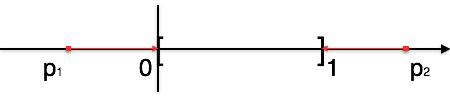
\includegraphics[width=0.9\textwidth]{img/projection_onto_c.png}
        \caption[Clipping to the set $C$]{\label{fig:projection_onto_c} A point $p_{1} < 0$ is clipped to $0$, whereas a point $p_{2} > 1$ is clipped to $1$.}
    \end{figure}

    \begin{remark}
        \begin{itemize}
            \item By projecting onto $C$, we also need to take care about the limits in \ref{eq:limits}. For that we set $u(i, j, 1) = 1$ and $u(i, j, S) = 0$ in each projection. Or similarly, using for instance the programming language C++, we have $u(i, j, 0) = 1$ and $u(i, j, S-1) = 0$.
            \item In the case of our framework - acting in a discrete cube $\mathcal{G}$ - equation \ref{ex:clipping} can be regarded as
                $$
                    u^{n+1}_{i,j,k} = \min\{1, \max \{ 0, u^{n}_{i,j,k} \} \}.
                $$
        \end{itemize}
    \end{remark}

    \subsection{The projection onto $K$} % (fold)
    \label{sub:the_projection_onto_K}

        Projecting onto $K$ is more involved than the projection onto $C$, since $K$ takes into account local and non-local constraints. In other words, the set $K$ is an intersection of several convex sets. The projection onto the intersection of convex sets can be done by Dykstra's projection algorithm. The idea behind this algorithm is to project onto each set alternatingly in a step $n$ and store the error, which is made in this iteration step. Before the projection in the $n+1$-th step is done, the vector which should be projected is reduced by the error made in the previous step. To fully understand this scheme, we first give the definition which was first proposed by Boyle and Dykstra in \cite{dykstra-et-al-aors14}, where one can also find a proof of convergence. Afterwards, we will provide and discuss the algorithm and additionally show an example.

        \begin{algorithm}
        \label{alg:dykstra}
            Consider $P$ convex sets with $\mathbb{R}^{n} \ni X = X_{1} \cap X_{2} \cap ... \cap X_{P}$. Let $\Pi_{i}$ denote the projection onto the i-th set for $i = 1, ..., P$. And let $u_{c} \in \mathbb{R}^{n}$ be the current estimate with $u_{c} \notin X$, $u_{i}^{k} \in \mathbb{R}^{n}$ for $i = 0, ..., P$ and $v_{i}^{k} \in \mathbb{R}^{n}$ for $i = 1, ..., P$ and $k = 1, 2, ...$, where $k$ denotes the number of iterations. Then the algorithm finds the (only) $u^{\ast} \in X$, such that

            $$
                ||u^{\ast} - u_{c}||^{2} \le ||u - u_{c}||^{2} \,\,\, \forall u \in X.
            $$

            For $k = 1, 2, ...$ set $u^{0}_{P} = u_{c}$ and $v^{0}_{i} = 0$ for all $i = 1, ..., P$. Then iterate until convergence (e.g. $||u_{0}^{k} - u_{P}^{k}||_{2} \le \varepsilon$ with $\varepsilon$ small):

            \begin{eqnarray}
                &u_{0}^{k} = &u_{P}^{k-1}, \notag \\
                &\textnormal{for} \,\, &i = 1, 2, ..., P: \notag \\
                &&u_{i}^{k} = \Pi_{i}(u_{i-1}^{k} - v_{i}^{k-1}), \notag \\
                &&v_{i}^{k} = u_{i}^{k} - (u_{i-1}^{k} - v_{i}^{k-1}). \notag
            \end{eqnarray}
        \end{algorithm}

        \begin{theorem}[Convergence]
            The sequence $u_{0}^{k}$ in algorithm \ref{alg:dykstra} converges to the (only) point $u \in X$.
        \end{theorem}
        As mentioned, the proof for the theorem can be found in \cite{dykstra-et-al-aors14}.

        % Recalling algorithm \ref{alg:dykstra}, we see that in each iteration step $k$ we project the current vector $u_{i-1}^{k}$ minus the error we made in the previous step, onto the i-th set. Afterwards, we update the error vector $v_{i}^{k}$. As illustrated in (BILD!!!), we project alternatingly on each set. At the end we convergence to the (only) point in $K$.

        Now, that we know how the projection onto the entire set $K$ can be implemented, we need to discuss how a projection onto the subsets of $K$ can be computed. First let us give a decomposition of $K$ into two several sets.
    % subsection the_projection_onto_K (end)

    \subsection{Decomposition of $K$} % (fold)
    \label{sub:decomposition_of_K}
        
        We will decompose the set $K$ into sets $K_{p}$ and $K_{nl}$, where the first resembles the local constraint, or more precisely, a parabola constraint and the second corresponds to the non-local constraint. Overall, we have $K = K_{p} \cap K_{nl}$ with

    \begin{equation}
        % &K_{p}& = \bigg\{ p^{3}(i,j,k) \ge \frac{p^{1}(i,j,k)^{2} + p^{2}(i,j,k)^{2}}{4} - \lambda(\frac{k}{M} - f(i,j))^{2} \bigg\} \,\,\, \forall i, j, k \notag \\
        K_{p} = \bigg\{ p^{t}(i, j, k) \ge \frac{||p^{x}(i, j, k)||^{2}}{4} - \lambda(\frac{k}{M} - f(i,j))^{2} \bigg\} \,\,\, \forall i, j, k \label{eq:parabola}
        % \Longleftrightarrow &K_{p}& = \bigg\{ p^{t}(i, j, k) \ge \frac{||p^{x}(i, j, k)||^{2}}{4} - \lambda(\frac{k}{M} - f(i,j))^{2} \bigg\} \,\,\, \forall i, j, k \label{eq:parabola}
    \end{equation}

    where $p^{t}(i, j, k) = p^{3}(i, j, k)$ and $p^{x}(i, j, k) = (p^{1}(i, j, k), p^{2}(i, j, k))^{T}$. For the non-local constraint we have

    \begin{equation}
        K_{nl} = \bigg\{ \left| \sum_{k_{1} \le k \le k_{2}} p^{x}(i, j, k) \right| \le \nu \bigg\} \,\,\, \forall i, j, k_{1} \le k \le k_{2}. \label{eq:nonlocal}
    \end{equation}

    We will now deduce the projection on these two sets. Let us start with the projection onto the parabola.
    %Since $K_{p}$ is an intersection of $P \cdot N \cdot M$ set and $K_{nl}$ is an intersection of $P \cdot N \cdot (\frac{M(M-1)}{2} + M)$ sets we need an algorithm which can handle the projection of a point onto (convex) sets. First let us introduce the projections onto $K_{p}$ and $K_{nl}$.

    % subsection decomposition_of_K (end)

    \subsection{Projection onto $K_{p}$}

        Since the projection onto the set $K_{p}$ is pointwise we want to drop the indices $(i, j, k)$. Note that we do not necessarily need that a $p^{x}$ is an element of $\mathbb{R}^{2}$. The following derivation holds for a larger class of problems namely having $p^{x} \in \mathbb{R}^{n}$. Let $\alpha > 0$, $p^{x} \in \mathbb{R}^{n}$, $p^{t} \in \mathbb{R}$ and $p = (p^{x}, p^{t})^{T} \in \mathbb{R}^{n} \times \mathbb{R}$. Assume that $p_{0}^{t} < \alpha ||p_{0}^{x}||_{2}^{2}$ holds for a point $p_{0} \in \mathbb{R}^{n}\times\mathbb{R}$. Then the projection of $p_{0}$ onto the parabola $\alpha ||p_{0}^{x}||_{2}^{2}$ can be written as the following minimization problem

            \begin{eqnarray}
                &\min\limits_{p \in \mathbb{R}^{n} \times \mathbb{R}}& \frac{1}{2} ||p - p_{0}||_{2}^{2} \notag \\
                &\textnormal{subject to}& p^{t} \ge \alpha||p^{x}||_{2}^{2} \notag
            \end{eqnarray}

        % Defining $f(p) = \frac{(p - p_{0})^{2}}{2}$ and $g(p) = p^{t} - \alpha ||p^{x}||_{2}^{2}$ the above convex optimization problem is equivalent to

        %     \begin{eqnarray}
        %         &\min\limits_{p \in \mathbb{R}^{n} \times \mathbb{R}}& f(p) \notag \\
        %         &\textnormal{subject to}& g(p) \ge 0 \notag
        %     \end{eqnarray}

        To find the solution of this optimization problem we introduce a Lagrange Multiplier $\mu \in \mathbb{R}$ and define the Lagrangian as

        \begin{equation}
            \mathcal{L}(p, \mu) = \frac{(p - p_{0})^{2}}{2} - \mu \bigg( p^{t} - \alpha||p^{x}||_{2}^{2} \bigg).
        \end{equation}

        We are seeking to minimize $\mathcal{L}(p, \mu)$ over all $p$ and $\mu$. The minimization problem we consider is convex, because our function to optimize is convex, the inequality constraint is convex and the feasible set $\mathbb{R}^{n} \times \mathbb{R}$ is also convex. For that, we know that computing a critical point of the Lagrangian function $\mathcal{L}$ also leads to a global optimum of the optimization problem itself. We compute a critical point with
        % Setting $\nabla \mathcal{L}(p, \mu) = 0$ we derive a global minimum, since our function to optimize is convex, the inequality constraint is convex and the feasible set $\mathbb{R}^{n} \times \mathbb{R}$ is also convex. We set

        \begin{equation}
            \nabla \mathcal{L}(p, \mu) =
            \begin{pmatrix}
                \partial_{p^{x}} \mathcal{L}(p, \mu) \\
                \partial_{p^{t}} \mathcal{L}(p, \mu) \\
                \partial_{\mu} \mathcal{L}(p, \mu)
            \end{pmatrix} = 
            \begin{pmatrix}
                p^{x} - p_{0}^{x} + \mu 2 \alpha p^{x} \\
                p^{t} - p_{0}^{t} - \mu \\
                p^{t} - \alpha||p^{x}||_{2}^{2}
            \end{pmatrix}
            = 0. \label{eq:linearSystem}
        \end{equation}

        That means, we need to solve a linear system. The first equation gives us

        \begin{equation}
            p_{0}^{x} = (\mu 2 \alpha + 1) p^{x} \Longleftrightarrow p^{x} = \frac{p_{0}^{x}}{\mu 2 \alpha + 1}, \label{eq:1stequ}
        \end{equation}

        and the second equation leads us to

        \begin{equation}
            p^{t} = p_{0}^{t} + \mu. \label{eq:2ndequ}
        \end{equation}

        % We can solve this system in two ways:
        In the following we discuss two different possibilities how the system \ref{eq:linearSystem} can be solved.
        \begin{enumerate}
            \item Plugging the equalities \ref{eq:1stequ} and \ref{eq:2ndequ} into the third line of equation \ref{eq:linearSystem}, we get

        \begin{eqnarray}
            p^{t} - \alpha||p^{x}||_{2}^{2} &\Longleftrightarrow& p_{0}^{t} + \mu - \alpha \bigg|\bigg|\frac{p_{0}^{x}}{\mu 2 \alpha + 1}\bigg|\bigg|_{2}^{2} = 0 \Longleftrightarrow p_{0}^{t} + \mu - \frac{\alpha}{(\mu 2 \alpha + 1)^{2}} ||p_{0}^{x}||_{2}^{2} = 0 \notag \\
            &\overbrace{\Longleftrightarrow}^{\cdot (\mu2\alpha + 1)^{2}}& (\mu 2 \alpha + 1)^{2} p_{0}^{t} + (\mu 2 \alpha + 1)^{2} \mu - \alpha ||p_{0}^{x}||_{2}^{2} = 0 \notag \\
            &\Longleftrightarrow& (4 \mu^{2} \alpha^{2} + 4 \mu \alpha + 1) p_{0}^{t} + 4 \mu^{3} \alpha^{2} + 4 \mu^{2} \alpha + \mu - \alpha ||p_{0}^{x}||_{2}^{2} = 0 \notag \\
            &\Longleftrightarrow& 4 \alpha^{2} \mu^{3} + \mu^{2} (4 \alpha^{2} p_{0}^{t} + 4 \alpha) + \mu (4 \alpha p_{0}^{t} + 1) + p_{0}^{t} - \alpha ||p_{0}^{x}||_{2}^{2} = 0. \notag
        \end{eqnarray}

        Defining a function
            $$
                h(\mu) = 4 \alpha^{2} \mu^{3} + \mu^{2} (4 \alpha^{2} p_{0}^{t} + 4 \alpha) + \mu (4 \alpha p_{0}^{t} + 1) + p_{0}^{t} - \alpha ||p_{0}^{x}||_{2}^{2},
            $$
        we are seeking for the zeroes of $h$. Computing the zeroes can efficiently be established by using Newton's algorithm defined by

        \begin{equation}
            \mu^{k+1} = \mu^{k} - \frac{h(\mu)}{h^{'}(\mu)}, \label{eq:newton}
        \end{equation}

        for $k = 1, 2, ...$.

        If we set
        $$
            h(\mu) = 4 \alpha^{2} \mu^{3} + \mu^{2} (4 \alpha^{2} p_{0}^{t} + 4 \alpha) + \mu(4 \alpha p_{0}^{t} + 1) + p_{0}^{t} - \alpha ||p_{0}^{x}||_{2}^{2},
        $$
        the first derivative of $h$ is given by
        $$
            h^{'}(\mu) = 12 \alpha^{2} \mu^{2} + 2 \mu (4 \alpha^{2} p_{0}^{t} + 4 \alpha) + (4 \alpha p_{0}^{t} + 1).
        $$
        Overall, we get the update equation for a $\mu^{k+1}$ with
            \begin{equation}
                \mu^{k+1} = \mu^{k} - \frac{4 \alpha^{2} \mu^{3} + \mu^{2} (4 \alpha^{2} p_{0}^{t} + 4 \alpha) + \mu(4 \alpha p_{0}^{t} + 1) + p_{0}^{t} - \alpha ||p_{0}^{x}||_{2}^{2}}{12 \alpha^{2} \mu^{2} + 2 \mu (4 \alpha^{2} p_{0}^{t} + 4 \alpha) + (4 \alpha p_{0}^{t} + 1)}.
            \end{equation}
        In \cite{Chambolle-et-al-10} they suggest setting $\mu^{0} = \max \{ 0, - \frac{2 p_{0}^{t}}{3} \}$, where they state that Newton's method converges within 7-10 iterations to a quite accurate solution.\\
        The projected vector $p$ of our problem is then given by
            \begin{equation}
                p = \bigg( \frac{p_{0}^{x}}{\mu 2 \alpha + 1}, p_{0}^{t} + \mu \bigg), \label{eq:newtonSolution}
            \end{equation}
        which we get from equations \ref{eq:1stequ} and \ref{eq:2ndequ}. We did not apply this method to our framework, since the primal-dual algorithm will be extremley slow in the case of this framework. Having a few iterations of Newton's algorithm in each iteration step would generate more overhead and for that would decelerate the program. Further, Newton's method is inexact and as it turns out, the second approach to this problem will lead to an exact solution, which can be computed within one loop of straightforward computations.

        \item For the second approach we note that \ref{eq:1stequ} and \ref{eq:2ndequ} hold and the third equation in \ref{eq:linearSystem} can be expressed with
        \begin{equation}
            p^{t} = \alpha ||p^{x}||_{2}^{2} \Longleftrightarrow \alpha ||p^{x}||_{2}^{2} = \underbrace{p_{0}^{t} + \mu}_{p^{t}}. \label{eq:tmp1}
        \end{equation}
        With equation \ref{eq:1stequ} we can also compute the solution of $\mu$ by using that

        \begin{eqnarray}
            p^{x} = \frac{p_{0}^{x}}{\mu 2 \alpha + 1} &\Longleftrightarrow& ||p^{x}||_{2} = \bigg|\bigg| \frac{p_{0}^{x}}{1 + 2 \alpha \mu} \bigg|\bigg|_{2} \Longleftrightarrow ||p^{x}||_{2} = \frac{1}{1 + 2 \alpha \mu} ||p_{0}^{x}||_{2} \notag \\
            &\Longleftrightarrow& \frac{1}{1 + 2 \alpha \mu} = \frac{||p^{x}||_{2}}{||p_{0}^{x}||_{2}} \notag \\
            &\Longleftrightarrow& 1 + 2\alpha\mu = \frac{||p_{0}||_{2}}{||p_{x}||_{2}} \notag \\
            &\Longleftrightarrow& 2 \alpha \mu = \frac{||p_{0}^{x}||_{2}}{||p^{x}||_{2}} - 1 \notag \\
            &\Longleftrightarrow& \mu = \frac{1}{2 \alpha} \bigg( \frac{||p_{0}^{x}||_{2}}{||p^{x}||_{2}} \bigg) - \frac{1}{2\alpha}. \notag
        \end{eqnarray}

        Using the solution of $\mu$ in \ref{eq:tmp1} we get

        \begin{eqnarray}
            \alpha ||p^{x}||_{2}^{2} = p_{0}^{t} + \frac{1}{2 \alpha} \bigg( \frac{||p_{0}^{x}||_{2}}{||p^{x}||_{2}} \bigg) - \frac{1}{2\alpha} &\overbrace{\Longleftrightarrow}^{\cdot 2 \alpha ||p^{x}||_{2}}& 2 \alpha^{2} ||p^{x}||_{2}^{3} = 2 \alpha ||p^{x}||_{2} p_{0}^{t} + ||p_{0}^{x}||_{2} - ||p^{x}||_{2} \notag \\
            &\Longleftrightarrow& 2 \alpha^{2} ||p^{x}||_{2}^{3} + 2\alpha||p^{x}||_{2} - 2\alpha p_{0}^{t} ||p^{x}||_{2} - ||p_{0}^{x}||_{2} = 0. \notag \\
            &\Longleftrightarrow& 2 \alpha^{2} ||p^{x}||_{2}^{3} + (1 - 2 \alpha p_{0}^{t}) ||p^{x}||_{2} - ||p_{0}^{x}||_{2} = 0. \notag \\
            &\overbrace{\Longleftrightarrow}^{\cdot 4 \alpha}& 8 \alpha^{3} ||p^{x}||_{2}^{3} + 4 \alpha (1 - 2 \alpha p_{0}^{t}) ||p^{x}||_{2} - 4 \alpha ||p_{0}^{x}||_{2} = 0. \notag \\
            &\Longleftrightarrow& (2 \alpha ||p^{x}||_{2})^{3} + 2 (1 - 2 \alpha p_{0}^{t}) 2 \alpha ||p^{x}||_{2} - 4 \alpha ||p_{0}^{x}||_{2} = 0. \notag \\
            &\Longleftrightarrow& t^{3} + 3bt - 2a = 0, \label{eq:cubic}
        \end{eqnarray}

        with $a = 2 \alpha ||p_{0}^{x}||_{2}$, $b = \frac{2}{3}(1 - 2 \alpha p_{0}^{t})$ and $t = 2 \alpha ||p^{x}||_{2}$.\\
        The cubic equation \ref{eq:cubic} in $t$ can efficiently be solved using the analytical formula for solving cubic equation published by J. P. McKelvey in 1984 in \cite{kelvey-ajp}.

        \end{enumerate}

        The result of the work mentioned is summarized in the following algorithm. Notice that we already computed the factors $a$ and $b$. The others follow with \cite{kelvey-ajp}.

            \begin{algorithm}

                If already $p_{0}^{t} \ge \alpha ||p_{0}^{x}||_{2}^{2}$, the solution is $(p^{x}, p^{t}) = (p_{0}^{x}, p_{0}^{t})$. Otherwise, with $a = 2 \alpha ||p_{0}^{x}||_{2}$, $b = \frac{2}{3} (1 - 2 \alpha p_{0}^{t})$, and

                    \[
                        d =
                            \begin{dcases*}
                                a^{2} + b^{3} & \textnormal{if $b \ge 0$}\\
                                (a - \sqrt{-b}^{3})(a + \sqrt{-b}^{3}) & \textnormal{else}
                            \end{dcases*}
                    \]

                set

                    \[
                        v =
                            \begin{dcases*}
                                c - \frac{b}{c} \,\, \textnormal{with} \,\, c = \sqrt[3]{a + \sqrt{d}} & \textnormal{if $d \ge 0$}\\
                                2 \sqrt{-b} \cos \bigg( \frac{1}{3} \arccos \frac{a}{\sqrt{-b}^{3}} \bigg) & \textnormal{else}.
                            \end{dcases*}
                    \]

                If $c = 0$ in the first case, set $v = 0$. The solution is then given by

                    \[
                        p^{x} =
                            \begin{dcases*}
                                \frac{v}{2\alpha} \frac{p_{0}^{x}}{||p_{0}^{x}||_{2}} & \textnormal{if $p_{0}^{x} \ne 0$}\\
                                0 & \textnormal{else}
                            \end{dcases*}
                    \]

                and $p^{t} = \alpha ||p^{x}||_{2}^{2}$.
            \end{algorithm}

        The above method states that the projection onto the parabola can be done by one cycle of straightforward computations. The implementation of it is quite simple and computation time is fast. Compared to Newton's algorithm, which is inexact, we get a exact solution and save a huge amount of run-time.

    \subsection{Projection onto $K_{nl}$}

        This set is a combination of non-local constraints, meaning that in a fixed point $(i, j, k)$ we sum up for all possible combinations $k_{1} \le k \le k_{2}$ for all $k, k_{1}, k_{2} = 1, ..., S$. For that reason you can not project pointwise. Let us first present the algorithm:

        \begin{algorithm}[Soft Shrinkage Scheme]
        \label{alg:softshrinkage}
            Let $p^{i}_{k} = (p^{1}(i, j, k), p^{2}(i, j, k))^{T} \in \mathbb{R}^{2}$, $p^{i} = (p^{i}_{1}, ..., p^{i}_{S})^{T} \in \mathbb{R}^{2 \times S}$ for all $i = 1, 2, ...$. Then the projection $p^{n+1}$ of a $p^{n}$ - for an arbitrary, fixed pair $(k_{1}, k_{2})$ with $1 \le k_{1} \le k \le k_{2} \le S$ - is computed by:

                \[
                    p^{n+1} =
                        \begin{dcases*}
                            p^{n} + \frac{s - \tilde{s}}{k_{2} - k_{1} + 1} & \textnormal{if $k_{1} \le k \le k_{2}$}, \\
                            p^{n} & \textnormal{else},
                        \end{dcases*}
                \]

            where $s \in \mathbb{R}^{2}, \tilde{s} \in \mathbb{R}^{2}$ with

                $$\tilde{s} = \sum_{k_{1} \le k \le k_{2}} p^{n}_{k}$$

            and

                \[
                    s =
                        \begin{dcases*}
                            \tilde{s} & \textnormal{if $||\tilde{s}||_{2} \le \nu$},\\
                            \Pi_{||\cdot||_{2} \le \nu}(\tilde{s}) = \frac{\nu}{||\tilde{s}||_{2}} \tilde{s} & \textnormal{else}.
                        \end{dcases*}
                \]

        \end{algorithm}

        Since this procedure needs a clarification, we need the KKT conditions. Following the notation, definition and theorem of \cite{Nocedal-Wright}, we consider the optimization problem:

            \begin{equation}
                \min_{x \in \mathbb{R}^{n}} \, f(x) \,\,\,\,\, \textnormal{subject to} \,\,\,
                \begin{dcases*}
                    c_{i}(x) = 0 & $i \in \mathcal{E}$, \\
                    c_{i}(x) \ge 0 & $i \in \mathcal{I}$,
                \end{dcases*}
                \label{eq:basic_optimization_problem}
            \end{equation}
        where $f$ and for all $i \in \mathcal{E} \cup \mathcal{I}$ the functions $c_{i}$ are smooth, real-valued functions on a subset of $\mathbb{R}^{n}$. Further, $\mathcal{E}$ and $\mathcal{I}$ denote two finite sets of indices. Here, $f$ is the objective function, whereas the $c_{i}$ for $i \in \mathcal{E}$ are the equality constraints and $c_{i}$ with $i \in \mathcal{I}$ the inequality constraints. We further want to define the feasible set $\Omega$. As stated in section \ref{sec:convex_optimization_and_convex_analysis} this set is the set of all points, which satisfy the constraints $c_{i}$ for all $i$. Then we have
            \begin{equation}
                \Omega = \{ x \,\, | \,\, c_{i}(x) = 0, \,\, i \in \mathcal{E}; \,\, c_{i} \ge 0, \,\, i \in \mathcal{I} \}.
                \label{eq:feasible_set_omega}
            \end{equation}
        We rewrite our optimization problem in terms of the set $\Omega$ to
            $$
                \min_{x \in \Omega} f(x).
            $$

        Additionally, we want to define the so called active set for the constraint functions.

        \begin{definition}[Active Set]
            \label{def:active_set}
            The active set $\mathcal{A}(x)$ at any feasible $x$ consists of the equality constraint indices from $\mathcal{E}$ together with the indices of the inequality constraints $i$, for which $c_{i}(x) = 0$, that is
                \begin{equation}
                    \mathcal{A}(x) = \mathcal{E} \cup \{ i \in \mathcal{I} | c_{i}(x) = 0 \}
                    \label{eq:active_set}
                \end{equation}
        \end{definition}

        We call a inequality constraint active if $c_{i} = 0$ and inactive if $c_{i} > 0$, for a $i \in \mathcal{I}$. The definition of the active set is an important basis for the following definition.

        \begin{definition}[LICQ]
            \label{def:licq}
            Given the point $x$ and the active set $\mathcal{A}(x)$, we say that the linear independence constraint qualification (LICQ) holds if the set of active constraint gradients
                $$
                    \{ \nabla c_{i}(x), \, i \in \mathcal{A}(x) \}
                $$
            is linearly independent.
        \end{definition}

        Then, we can propose the first-order necessary conditions, which are also well known as the Karush-Kuhn-Tucker (KKT) optimality conditions.

        \begin{theorem}[Karush-Kuhn-Tucker Optimality Conditions]
        \label{the:kkt_conditions}
            Suppose that $x^{\ast}$ is a local solution of equation \ref{eq:basic_optimization_problem}, that the
            functions $f$ and $c_{i}$ are continuously differentiable, and that the LICQ holds at $x^{\ast}$. Then there is a Lagrange multiplier vector $\lambda^{\ast}$, with components $\lambda_{i}^{\ast}, i \in \mathcal{E} \cup \mathcal{I}$, such that the following conditions are satisfied at $(x^{\ast}, \lambda^{\ast})$.
            \begin{subequations}
                \begin{align}
                    \nabla_{x}\mathcal{L}(x^{\ast}, \lambda^{\ast}) &= 0, \label{eq:stationarity} \\
                    c_{i}(x^{\ast}) &= 0, \,\,\,\,\, \textnormal{for all} \, i \in \mathcal{E}, \\
                    c_{i}(x^{\ast}) &\ge 0, \,\,\,\,\, \textnormal{for all} \, i \in \mathcal{I}, \\
                    \lambda_{i}^{\ast} &\ge 0, \,\,\,\,\, \textnormal{for all} \, i \in \mathcal{I}, \\
                    \lambda_{i}^{\ast}c_{i}(x^{\ast}) &= 0, \,\,\,\,\, \textnormal{for all} \, i \in \mathcal{E} \cup \mathcal{I}.\label{eq:complementary_conditions}
                \end{align}
                \label{eq:kkt_conditions}
            \end{subequations}
        \end{theorem}

        \begin{remark}
            The last condition \ref{eq:complementary_conditions} in the theorem is also known as the complementary slackness condition. It implies that either the $i$-th constraint is active or $\lambda_{i}^{\ast} = 0$. It is also possible, that both are zero.
        \end{remark}

    A proof of theorem \ref{the:kkt_conditions} can, for instance, be found in \cite{Nocedal-Wright}. Let us now proof, that the algorithm \ref{alg:softshrinkage} is valid, by using the KKT conditions.

    \begin{proof}
        Let $\tilde{s}, s, p_{k}, \tilde{p}_{k} \in \mathbb{R}^{2}$ and $p, \tilde{p} \in \mathbb{R}^{2 \times M}$ have the same form as in algorithm \ref{alg:softshrinkage}. For a fixed pair $(k_{1}, k_{2})$ we face the following optimization problem:

        \begin{subequations}
            \begin{align}
            \min\limits_{p \in \mathbb{R}^{2 \times M}} &\frac{1}{2} ||p - \tilde{p}||^{2}_{2} \\
            \textnormal{subject to} \,\,\, &\bigg{|} \bigg{|} \sum_{k_{1} \le k \le k_{2}} p_{k} \bigg{|} \bigg{|}_{2} \le \nu. \label{eq:inequalityConstraint}
            \end{align}
            \label{eq:optimization_problem}
        \end{subequations}

        The problem states that we try to find the closest $p$ to $\tilde{p}$ whose components fullfil the inequality constraint in \ref{eq:inequalityConstraint}, which can also be written as
            $$
                \bigg{|} \bigg{|} \sum_{k_{1} \le k \le k_{2}} p_{k} \bigg{|} \bigg{|}_{2} - \nu \le 0.
            $$

        % If we define functions
        %     $$
        %         f(p) = \sum_{k = 1}^{M} \frac{(p_{k} - \tilde{p}_{k})^{2}}{2}, \,\,\,\,\, g_{i}(p) = \frac{1}{2} \nu^{2} - \frac{1}{2} ||\tilde{s}||_{2}^{2} \tilde{s}
        %     $$
        % for i = 1, then an equivalent formulation of the system \ref{eq:optimization_problem} would be
        % \begin{subequations}
        %     \begin{align}
        %         &\min\limits_{p \in \mathbb{R}^{2 \times M}} &f(p) \\
        %         &\textnormal{subject to} &g_{i}(p) \ge 0,
        %     \end{align}
        %     \label{eq:problem_to_solve}
        % \end{subequations}

        % with the set of indices $\mathcal{I} = \{1\}$. Note, that we have no equality constraints in this optimization problem. Since this optimization problem only has one constraint, we drop the index for the function $g$ in the following. %Since the function $g(p)$ for a fixed pair $(k_{1}, k_{2})$ is a real-valued function, the active set for this problem is
            % $$
            %     \mathcal{A}(x) = \{ i \in \mathcal{I} \, | \, g_{i}(p) = 0 \}.
            % $$
        % With this we want to show, that the LICQ definition is fullfild. For this let us compute
        %     \begin{eqnarray}
        %         \{ \nabla g_{i}(x), \, i \in \mathcal{A}(x) \} &=& \bigg\{ \nabla \bigg( \frac{1}{2} \nu^{2} - \frac{1}{2} \bigg{|} \bigg{|} \sum_{k_{1} \le k \le k_{2}} p_{k} \bigg{|} \bigg{|}_{2}^{2} \bigg) \bigg\} \notag \\
        %         &=& \bigg\{ - \sum_{k_{1} \le k \le k_{2}} p_{k} \bigg\} \notag \\
        %         &=& \{-\tilde{s}\} \notag
        %     \end{eqnarray}

        The feasible set for a point $(k_{1}, k_{2})$ of this optimization problem is given by
            $$
                \mathcal{F}_{p} = \{ p \in Y \, | \, \sum_{k_{1} \le k \le k_{2}} p_{k} \,\, \forall \, k_{1} \le k \le k_{2} \, \textnormal{with} \, k = 1, ..., S \}.
            $$
        If $\tilde{p} \in \mathcal{F}_{p}$, the inequality constraint is fullfild and for that $p = \tilde{p}$ leads to the minimal energy, which is zero. For that reason, we only consider points $\tilde{p} \notin \mathcal{F}_{p}$.

        %Clearly, $\tilde{s}$ is, linearly independent (of itself) and we can make use of the KKT conditions.
        Let us introduce a Lagrange multiplier variable $\lambda \in \mathbb{R}$ and observe the Lagrange function
        \begin{equation}
            \mathcal{L}(p, \lambda) = f(p) - \lambda g(p) = \sum_{k = 1}^{M} \frac{(p_{k} - \tilde{p}_{k})^{2}}{2} - \lambda \frac{1}{2} \nu^{2} - \frac{1}{2} - \bigg{|} \bigg{|} \sum_{k_{1} \le k \le k_{2}} p_{k} \bigg{|} \bigg{|}_{2}.
        \end{equation}

        Considering equation \ref{eq:stationarity} and assume that $p^{\ast}_{k} = \tilde{p}_{k} + \frac{s - \tilde{s}}{k_{2} - k_{1} + 1}$ is a feasible point, that satisfies LICQ and is a local solution of system \ref{eq:optimization_problem}, together with a optimal $\lambda^{\ast}$. Then we have

        \begin{equation}
            \nabla_{p} \mathcal{L}(p^{\ast}, \lambda^{\ast}) = \nabla_{p} f(p^{\ast}) + \lambda \nabla_{p} g(p^{\ast}) =
            \underbrace{\begin{pmatrix}
                p^{\ast}_{1} - \tilde{p}_{1} \\
                 \\
                \vdots \\
                 \\
                \vdots \\
                 \\
                \vdots \\
                 \\
                p^{\ast}_{S} - \tilde{p}_{S}
            \end{pmatrix}}_{\in \mathbb{R}^{S}}
            + \lambda^{\ast}
            \underbrace{\begin{pmatrix}
                0 \\
                \vdots \\
                \sum\limits_{k_{1} \le k \le k_{2}} p^{\ast}_{k} \\
                \vdots \\
                \sum\limits_{k_{1} \le k \le k_{2}} p^{\ast}_{k} \\
                0 \\
                \vdots
            \end{pmatrix}}_{\in \mathbb{R}^{S}}
            = 0,
        \end{equation}

        where the zeroes in the last vector are obtain for all components where $k < k_{1}$ and $k > k_{2}$. For these lines we have

            $$
                p^{\ast}_{k} = \tilde{p}_{k} \,\,\, \textnormal{if} \,\, k < k_{1} \,\, \textnormal{and} \,\, k > k_{2}.
            $$
        We also have for such a point that $p^{\ast} \in \mathcal{F}_{p}$. With this, let us take a closer look at the i-th line where $(\nabla_{p} g(p))_{i} \ne 0$. Then we have

            \begin{equation}
                p^{\ast}_{i} - \tilde{p}_{i} + \lambda^{\ast} \sum_{k_{1} \le k \le k_{2}} p^{\ast}_{k} = 0.
                \label{eq:ithRow}
            \end{equation}

        Further, we observe for the feasible point $p^{\ast}$ the following identity:
            \begin{eqnarray}
                \frac{1}{2} \bigg|\bigg|\sum_{k_{1} \le k \le k_{2}} p^{\ast}_{k}\bigg|\bigg|_{2}^{2} - \frac{1}{2} \nu^{2} &=& \frac{1}{2(k_{2} - k_{1} + 1)} \bigg|\bigg|\sum_{k_{1} \le k \le k_{2}} \tilde{p}_{k} + (s - \tilde{s})\bigg|\bigg|_{2}^{2} - \frac{1}{2} \nu^{2} \notag \\
                &=& \frac{1}{2} \bigg|\bigg|\sum_{k_{1} \le k \le k_{2}} \tilde{s} + s - \tilde{s}\bigg|\bigg|_{2}^{2} - \frac{1}{2} \nu^{2} = \frac{1}{2} \underbrace{||s||_{2}^{2}}_{= \nu^{2}} - \frac{1}{2} \nu^{2} = 0. \notag
            \end{eqnarray}
        This means, that the inequality constraint is active at the point $p^{\ast}$. Since, this is the case we show that the LICQ is fullfild for $p^{\ast}$. We have
            \begin{eqnarray}
                (\nabla g(p^{\ast}))_{i} = - \sum_{k_{1} \le k \le k_{2}} p^{\ast}_{k} &=& - \bigg( \sum_{k_{1} \le k \le k_{2}} \tilde{p}_{k} + \frac{\tilde{s} - s}{k_{2} - k_{1} + 1} \bigg) \notag \\
                &=& - \bigg( \sum_{k_{1} \le k \le k_{2}} \tilde{p}_{k} + \sum_{k_{1} \le k \le k_{2}} \frac{\tilde{s} - s}{k_{2} - k_{1} + 1} \bigg) \notag \\
                &=& - \bigg( \tilde{s} + \frac{k_{2} - k_{1} + 1}{k_{2} - k_{1} + 1} s - \tilde{s} \bigg) \notag \\
                &=& - s
            \end{eqnarray}
        Because, we only observe one vector, LICQ is always true for this $p^{\ast}$. It is left to compute $\lambda^{\ast}$ and show that it is greater or equal to zero. We have
            \begin{eqnarray}
                    &&p^{\ast}_{i} - \tilde{p}_{i} + \frac{\lambda^{\ast}}{k_{2} - k_{1} + 1} \sum_{k_{1} \le k \le k_{2}} p^{\ast}_{k} = \notag \\
                    &=& \tilde{p}_{i} + \frac{s - \tilde{s}}{k_{2} - k_{1} + 1} - \tilde{p}_{i} + \frac{\lambda^{\ast}}{k_{2} - k_{1} + 1} \sum_{k_{1} \le k \le k_{2}} \tilde{p}_{k} + \frac{s - \tilde{s}}{k_{2} - k_{1} + 1} \notag \\
                    &=& \frac{s - \tilde{s}}{k_{2} - k_{1} + 1} + \frac{\lambda^{\ast}}{k_{2} - k_{1} + 1} \bigg( \underbrace{\sum_{k_{1} \le k \le k_{2}} \tilde{p}_{k}}_{= \tilde{s}} + \underbrace{\sum_{k_{1} \le k \le k_{2}} \frac{s - \tilde{s}}{k_{2} - k_{1} + 1}}_{= \frac{(k_{2} - k_{1} + 1) (s - \tilde{s})}{k_{2} - k_{1} + 1} = s - \tilde{s}} \bigg) \notag \\
                    &=& \frac{s - \tilde{s}}{k_{2} - k_{1} + 1} + \frac{\lambda^{\ast}}{k_{2} - k_{1} + 1} (\tilde{s} + s - \tilde{s}) \notag \\
                    &=& \frac{s - \tilde{s}}{k_{2} - k_{1} + 1} + \frac{\lambda^{\ast}}{k_{2} - k_{1} + 1}s \notag \\
                    &=& \frac{1}{k_{2} - k_{1} + 1} (s - \tilde{s} + \lambda^{\ast}s) = 0 \label{eq:equalsZero}
                \end{eqnarray}

            Now we can solve for $\lambda^{\ast}$ using that the last equation \ref{eq:equalsZero} is equivalent to
                \begin{eqnarray}
                    (s - \tilde{s} + \lambda^{\ast} s) = 0 &\overbrace{\Longleftrightarrow}^{||\tilde{s}||_{2} > \nu}& \bigg(\frac{\nu}{||\tilde{s}||_{2}}\tilde{s} - \tilde{s} + \lambda^{\ast} \frac{\nu}{||\tilde{s}||_{2}}\tilde{s} \bigg) = 0 \notag \\
                    &\Longleftrightarrow& \tilde{s} \bigg( \frac{\nu}{||\tilde{s}||_{2}} - 1 + \lambda^{\ast} \frac{\nu}{||\tilde{s}||_{2}} \bigg) = 0 \notag \\
                    &\Longleftrightarrow& \frac{\nu}{||\tilde{s}||_{2}} - 1 + \lambda^{\ast} \frac{\nu}{||\tilde{s}||_{2}} = 0 \notag \\
                    &\Longleftrightarrow& \lambda^{\ast} \frac{\nu}{||\tilde{s}||_{2}} = 1 - \frac{\nu}{||\tilde{s}||_{2}} \notag \\
                    &\Longleftrightarrow& \lambda^{\ast} = \underbrace{\frac{||\tilde{s}||_{2}}{\nu}}_{> 1} - 1 > 0. \notag
                \end{eqnarray}

            In the last equation we used that $\tilde{s} = \sum\limits_{k_{1} \le k \le k_{2}} \tilde{p}_{k}$ and the fact we assumed $||\tilde{s}||_{2} > \nu$.

        % We set % state that the optimal $\lambda^{\ast}$ is of the form

        %     \begin{equation}
        %         \lambda^{\ast} = \frac{1}{k_{2} - k_{1} + 1} \bigg( \frac{\nu}{||\tilde{s}||_{2}} - 1 \bigg). \label{eq:lambda}
        %         % \lambda^{\ast} = \frac{\nu}{||\sum\limits_{k_{1} \le k \le k_{2}} p^{\ast}||_{2}} - 1. \label{eq:lambda}
        %     \end{equation}

        % with

            % $$\tilde{s} = \sum\limits_{k_{1} \le k \le k_{2}} \tilde{p}_{k}$$

        % Let us further define $s \in \mathbb{R}^{2}$ with

        %     \[
        %         s =
        %             \begin{dcases*}
        %                 \tilde{s} & \textnormal{if $||\tilde{s}||_{2} \le \nu$},\\
        %                 \Pi_{||\cdot||_{2} \le \nu}(\tilde{s}) = \frac{\nu}{||\tilde{s}||_{2}} \tilde{s} & \textnormal{else}.
        %             \end{dcases*}
        %     \]

        % We now distinguish between two cases:

        % \begin{enumerate}
        %     \item $||\tilde{s}||_{2} \le \nu$:\\
        %     Setting $p^{\ast}_{k} = \tilde{p}_{k} + \frac{s - \tilde{s}}{k_{2} - k_{1} + 1} = \tilde{p}_{k}$ for all $k_{1} \le k \le k_{2}$ and $s = \tilde{s}$ gives us in this case
        %         \begin{equation}
        %             g(p^{\ast}) = \frac{1}{2} \nu^{2} - \frac{1}{2} ||\sum_{k_{1} \le k \le k_{2}} p^{\ast}_{k}||_{2}^{2} \ge 0. \label{eq:caseOne}
        %         \end{equation}
        %     If equality holds in equation \ref{eq:caseOne}, we can choose an arbitrary $\lambda^{\ast} \ge 0$, so that condition \ref{eq:complementary_conditions} holds. We choose $\lambda^{\ast}$ to be
        %         \begin{equation}
        %             \lambda^{\ast} = \frac{||\tilde{s}||_{2}}{\nu} - 1.
        %             \label{eq:lambda}
        %          \end{equation}
        %     Since If $g(p^{\ast}) > 0$, the
        %     It follows for condition \ref{eq:complementary_conditions} that we can choose an arbitrary $\lambda^{\ast} \ge 0$ if we have equality in \ref{eq:caseOne} and $\lambda^{\ast} = 0$ else to derive the \underline{Dual Feasibility} condition. We set
        %         $$
        %             \lambda^{\ast} = 0.
        %         $$
        %     \item $||\sum\limits_{k_{1} \le k \le k_{2}} \tilde{p}_{k}||_{2} > \nu$:\\
        %     Here, we would violate the \underline{Primal Feasibility} condition if we set $p^{\ast}_{k} = \tilde{p}_{k}$ for all $k_{1} \le k \le k_{2}$. For this reason we choose
        %         $$
        %             p^{\ast}_{k} = \tilde{p}_{k} + \frac{s - \tilde{s}}{k_{2} - k_{1} + 1} \,\,\,\,\,\, \forall k_{1} \le k \le k_{2}
        %         $$
        %     We observe for the \underline{Primal Feasibility} condition that
        %         \begin{eqnarray}
        %             \frac{1}{2} ||\sum_{k_{1} \le k \le k_{2}} p^{\ast}_{k}||_{2}^{2} - \frac{1}{2} \nu^{2} &=& \label{eq:caseTwo} \\
        %             &=& \frac{1}{2(k_{2} - k_{1} + 1)} ||\sum_{k_{1} \le k \le k_{2}} \tilde{p}_{k} + (s - \tilde{s})||_{2}^{2} - \frac{1}{2} \nu^{2}\notag \\
        %             &=& \frac{1}{2} ||\sum_{k_{1} \le k \le k_{2}} \tilde{s} + s - \tilde{s}||_{2}^{2} - \frac{1}{2} \nu^{2} = \frac{1}{2} \underbrace{||s||_{2}^{2}}_{= \nu^{2}} - \frac{1}{2} \nu^{2} = 0. \notag
        %         \end{eqnarray}
            % Using this equality we already see that \underline{Complementary Slackness} is fullfild with a \underline{dual feasible} $\lambda^{\ast} \ge 0$. Since we set $p^{\ast}_{k} = \tilde{p}_{k} + \frac{s - \tilde{s}}{k_{2} - k_{1} + 1}$ we can plug $p^{\ast}$ into \ref{eq:ithRow} to derive $\lambda^{\ast}$. It follows
            %     \begin{eqnarray}
            %         &&p^{\ast}_{i} - \tilde{p}_{i} + \frac{\lambda^{\ast}}{k_{2} - k_{1} + 1} \sum_{k_{1} \le k \le k_{2}} p^{\ast}_{k} = \notag \\
            %         &=& \tilde{p}_{i} + \frac{s - \tilde{s}}{k_{2} - k_{1} + 1} - \tilde{p}_{i} + \frac{\lambda^{\ast}}{k_{2} - k_{1} + 1} \sum_{k_{1} \le k \le k_{2}} \tilde{p}_{k} + \frac{s - \tilde{s}}{k_{2} - k_{1} + 1} \notag \\
            %         &=& \frac{s - \tilde{s}}{k_{2} - k_{1} + 1} + \frac{\lambda^{\ast}}{k_{2} - k_{1} + 1} \bigg( \underbrace{\sum_{k_{1} \le k \le k_{2}} \tilde{p}_{k}}_{= \tilde{s}} + \underbrace{\sum_{k_{1} \le k \le k_{2}} \frac{s - \tilde{s}}{k_{2} - k_{1} + 1}}_{= \frac{(k_{2} - k_{1} + 1) (s - \tilde{s})}{k_{2} - k_{1} + 1} = s - \tilde{s}} \bigg) \notag \\
            %         &=& \frac{s - \tilde{s}}{k_{2} - k_{1} + 1} + \frac{\lambda^{\ast}}{k_{2} - k_{1} + 1} (\tilde{s} + s - \tilde{s}) \notag \\
            %         &=& \frac{s - \tilde{s}}{k_{2} - k_{1} + 1} + \frac{\lambda^{\ast}}{k_{2} - k_{1} + 1}s \notag \\
            %         &=& \frac{1}{k_{2} - k_{1} + 1} (s - \tilde{s} + \lambda^{\ast}s) = 0 \label{eq:equalsZero}
            %     \end{eqnarray}

            % Now we can solve for $\lambda^{\ast}$ using that the last equation \ref{eq:equalsZero} is equivalent to
            %     \begin{eqnarray}
            %         (s - \tilde{s} + \lambda^{\ast} s) = 0 &\overbrace{\Longleftrightarrow}^{||\tilde{s}||_{2} > \nu}& \bigg(\frac{\nu}{||\tilde{s}||_{2}}\tilde{s} - \tilde{s} + \lambda^{\ast} \frac{\nu}{||\tilde{s}||_{2}}\tilde{s} \bigg) = 0 \notag \\
            %         &\Longleftrightarrow& \tilde{s} \bigg( \frac{\nu}{||\tilde{s}||_{2}} - 1 + \lambda^{\ast} \frac{\nu}{||\tilde{s}||_{2}} \bigg) = 0 \notag \\
            %         &\Longleftrightarrow& \frac{\nu}{||\tilde{s}||_{2}} - 1 + \lambda^{\ast} \frac{\nu}{||\tilde{s}||_{2}} = 0 \notag \\
            %         &\Longleftrightarrow& \lambda^{\ast} \frac{\nu}{||\tilde{s}||_{2}} = 1 - \frac{\nu}{||\tilde{s}||_{2}} \notag \\
            %         &\Longleftrightarrow& \lambda^{\ast} = \underbrace{\frac{||\tilde{s}||_{2}}{\nu}}_{> 1} - 1 > 0. \notag
            %     \end{eqnarray}

        %     This satisfies the \underline{Dual Feasibility} condition.
        % \end{enumerate}

        % With the choices of $\tilde{s}, s$ and

        %     $$p^{\ast}_{k} = \tilde{p}_{k} + \frac{s - \tilde{s}}{k_{2} - k_{1} + 1} \,\,\,\,\,\, \forall k_{1} \le k \le k_{2}$$

        % we solved \ref{eq:ithRow} (\underline{Stationarity}). 
        Applying this procedure to each combination $(k_{1}, k_{2})$ and replacing $p^{\ast}$ by $p^{n+1}$, $\tilde{p}$ by $p^{n}$ respectively, we observe our algorithm.
        \qed
    \end{proof}

        % with $\lambda \in \mathbb{R}^{m}$ and $\lambda_{i} \ge 0$ for all $i = 1, ..., m$.
        % With this and the fact that the inequality constraint also holds for all $i = 1, ..., m$ the \underline{Primal} and the \underline{Dual Feasibility} are already fullfild.\\ 

        % Applying \underline{Stationarity} condition we have:

        % \begin{equation}
        %     \nabla \mathcal{L}(x^{*}, \lambda^{*}) = 0 \Longleftrightarrow - \nabla f(p^{*}) = \sum_{l = 1}^{m} \lambda^{*}_{l} \nabla g_{l}(p^{*}).
        % \end{equation}

        % And \underline{Complementary Slackness} telling us that

        % \begin{equation}
        %     \lambda^{*} g(p^{*}) = 0.% \bigg( \frac{1}{2} \bigg{|} \bigg{|} \sum_{k_{1} \le k \le k_{2}} (p^{1}(i, j, k), p^{2}(i, j, k))^{T} \bigg{|} \bigg{|}_{2}^{2} - \frac{1}{2} \nu^{2} \bigg) = 0.
        % \end{equation}

% Back to the convex set $K$ we find that this set is the intersection of several sets. In \ref{eq:localconst} you find local constraints, more precisely parabola constraints. This constraint is pixel wise. If the third component of a vector $p$ namely $p^{3}$ satisfies this inequality the vector $p$ already lies in the constraint set \ref{eq:localconst}. If not some computations need to be done. We'll come back to that later. \\
% On the other hand the set in \ref{eq:nonlocalconst} is more complicated and also needs special treatment. This set takes not only values from one fixed voxel into account but sums up several voxel from a range $k_{1}$ to $k_{2}$. In the end we need to have that $p \in K$ and $p$ must satisfy both constraints. \\

We presented and proved several projection methods to project onto the sets $C$ and $K$. As we will see in the chapter \ref{cha:applications_to_imaging} this approach needs a huge amount of memory and is extremley slow, even on a GPU. In the next section, we will present an alternative approach.
    % \section{An alternative approach} % (fold)
\label{sec:an_alternative_approach}
    
    In this section we present a formulation to solve the discrete Mumford-Shah Functional of subsection \ref{sub:the_mumford_shah_model_as_saddle_point_problem}. The idea is to decouple the set $K_{nl}$ to derive an alternative saddle-point problem, which can be solved with our primal-dual algorithm. Recalling the original problem, we had
        \begin{equation}
            \min_{u \in C} \max_{p \in K} \langle Au, p \rangle,
            \label{eq:standard_form}
        \end{equation}
    where we maximized over the whole set $K$, defined in equations \ref{eq:local_constraint} and \ref{eq:non_local_constraint}. As discussed in section \ref{sec:discrete_setting_ms}, this set is an intersection of several convex sets. We projected onto the non-local constraint, which was defined by
        $$
            K_{nl} = \left\{ \left| \sum_{k_{1} \le k \le k_{2}} p^{x}(i, j, k) \right| \le \nu \right\} \,\,\, \forall i, j, k_{1} \le k \le k_{2},
        $$
    where $p^{x}$ is defined as in subsection \ref{sub:decomposition_of_K}, using a soft-shrinkage scheme. This projection was used in each step of Dykstra's algorithm. We now want to solve this problem optimal by decoupling the non-local constraint. We note that in the following we drop the index representation for $p^{x}$. Instead of writting $p^{x}(i, j, k)$ we denote this by $p^{x}_{k}$ for a pair $(i,j)$ and all $k$. Decoupling means then, that we substitute $p^{x}_{k}$ by $s_{k_{1}, k_{2}}$ and introduce an additional constraint to take the bound on $\nu$ into account. We have
        \begin{equation}
            K_{nl} = \left\{ |s_{k_{1}, k_{2}}| \le \nu \,\,\, \textnormal{subject to} \,\,\, s_{k_{1}, k_{2}} = \sum_{k_{1} \le k \le k_{2}} p^{x}_{k} \right\}
            \label{eq:non_local_constraint_reloaded}
        \end{equation}
    for all combinations $1 \le k_{1} \le k \le k_{2} \le S$, $s_{k_{1}, k_{2}} \in \mathbb{R}^{2}$ and $s \in \mathbb{R}^{N \times M \times S \times 2}$, respectively. Alternatively, we can also denote this set by
        $$
            K_{nl} = \left\{ |s_{k_{1}, k_{2}}| \le \nu \,\,\, \textnormal{subject to} \,\,\, s_{k_{1}, k_{2}} - \sum_{k_{1} \le k \le k_{2}} p^{x}_{k} = 0 \right\}
        $$
    We further present an auxiliary variable $\mu_{k_{1}, k_{2}} \in \mathbb{R}^{2}$, which belongs to a $\mu \in \mathbb{R}^{N \times M \times S \times 2}$. We define a new function
        \begin{equation}
            \mathcal{L}(u, \mu, p, s) = \langle Au, p \rangle + \sum_{k_{1} = 1}^{S} \sum_{k_{2} = k_{1}}^{S} \langle \mu_{k_{1}, k_{2}}, s_{k_{1}, k_{2}} - \sum_{k_{1} \le k \le k_{2}} p^{x}_{k} \rangle,
        \end{equation}
    in which we added to our original problem an enforced term corresponding to the constraint in $K_{nl}$. Taking now into account, that the constraint is an equality constraint, we have that all $\mu_{k_{1}, k_{2}}$ can either be greater, less than or equal to zero. Additionally, we need to be sure, that the inequality $|s_{k_{1}, k_{2}}| \le \nu$ holds. Then we obtain the following equivalence:
        $$
            \min_{u \in C} \max_{p \in K} \langle Au, p \rangle \Longleftrightarrow \min_{\substack{u \in C \\ \mu_{k_{1}, k_{2}}}} \max_{\substack{p \in K_{p} \\ |s_{k_{1}, k_{2}}| \le \nu}} \mathcal{L}(u, \mu, p, s),
        $$
    which complies to
        \begin{equation}
            \min_{u \in C} \max_{p \in K} \langle \nabla u, p \rangle \Longleftrightarrow \min_{\substack{u \in C \\ \mu_{k_{1}, k_{2}}}} \max_{\substack{p \in K_{p} \\ |s_{k_{1}, k_{2}}| \le \nu}} \langle \nabla u, p \rangle + \sum_{k_{1} = 1}^{S} \sum_{k_{2} = 1}^{S} \langle \mu_{k_{1}, k_{2}}, \sum_{k_{1} \le k \le k_{2}} p^{x}_{k} - s_{k_{1}, k_{2}} \rangle,
            \label{eq:lagrange_problem}
        \end{equation}
    if we use $A = \nabla$ as in the other chapters. Let us proof this equivalence in the general case, where $A$ resemble a linear operator:

    \begin{proof}
        As we did not change either the properties on $u$ nor the set $C$, we assume for the rest of the proof, that we found an optimal value $u^{\ast}$. Further, assume we have a optimal value $s^{\ast}$, for which $|s^{\ast}_{k_{1}, k_{2}}| \le \nu$ for all possible combinations $(k_{1}, k_{2})$. Then, we do a case analysis:
        \begin{enumerate}
            \item If the equality
                $$
                    \sum_{k_{1} \le k \le k_{2}} p^{x}_{k} - s^{\ast}_{k_{1}, k_{2}} = 0,
                $$
            holds, the saddle-point problem reduces to
                $$
                    \max_{p \in K_{p}} \langle Au^{\ast}, p \rangle.
                $$
            If the equality does not hold, we distinguish between two other cases:
            \item Let $\sum\limits_{k_{1} \le k \le k_{2}} p^{x}_{k} < s^{\ast}_{k_{1}, k_{2}}$, then first note, that this is equivalent to
                $$
                    \left|\left|\sum_{k_{1} \le k \le k_{2}} p^{x}_{k}\right|\right| < |s^{\ast}_{k_{1}, k_{2}}|.
                $$
            But as $|s^{\ast}_{k_{1}, k_{2}}| \le \nu$ we already have
                $$
                    \left|\left|\sum_{k_{1} \le k \le k_{2}} p^{x}_{k}\right|\right| \le \nu.
                $$
            Further, we obtain the minimal value over all possible $\mu_{k_{1}, k_{2}}$ in this case only if we let $\mu_{k_{1}, k_{2}} \longrightarrow \infty$, for which the whole energy becomes $-\infty$. Since, the conditions according to the set $K_{nl}$ are met and to avoid having a energy with the value $-\infty$, we set $\mu_{k_{1}, k_{2}} = 0$ in this case. We get again
                $$
                    \max_{p \in K_{p}} \langle Au^{\ast}, p \rangle.
                $$
            \item Now, let $\sum\limits_{k_{1} \le k \le k_{2}} p^{x}_{k} > s^{\ast}_{k_{1}, k_{2}}$. In this case we could again set $\mu_{k_{1}, k_{2}} = 0$. Then the last term in \ref{eq:lagrange_problem} will not be considered. But with this we are not able to tell anything about the sum over the $p^{x}_{k}$. We know that
                $$
                    \left|\left|\sum_{k_{1} \le k \le k_{2}} p^{x}_{k}\right|\right| > |s^{\ast}_{k_{1}, k_{2}}|
                $$
            and from our assumption that $|s^{\ast}_{k_{1}, k_{2}}| \le \nu$. The only choice we have is to set
                $$
                    \sum_{k_{1} \le k \le k_{2}} p^{x}_{k} = s^{\ast}_{k_{1}, k_{2}}.
                $$
            With this we get
                $$
                    \max_{p \in K_{p}} \langle Au^{\ast}, p \rangle,
                $$
            and the $\mu_{k_{1}, k_{2}}$ can be chosen arbitrarily. This shows, that the two problems are equivalent.
        \end{enumerate}\qed
    \end{proof}

    Defining the function
    $$
        \mathcal{M}(u, \mu, p, s) = \langle Au, p \rangle + \sum_{k_{1} = 1}^{S} \sum_{k_{2} = 1}^{S} \langle \mu_{k_{1}, k_{2}}, \sum_{k_{1} \le k \le k_{2}} p^{x}_{k} - s_{k_{1}, k_{2}} \rangle
    $$

    leads to

        \begin{eqnarray}
            \frac{\partial \mathcal{M}(u, \mu, p, s)}{\partial u} &=& A^{T} p \\
            \frac{\partial \mathcal{M}(u, \mu, p, s)}{\partial p_{k}} &=& \sum_{k_{1}, k_{2}} \mu_{k_{1}, k_{2}} \\
            \frac{\partial \mathcal{M}(u, \mu, p, s)}{\partial \mu_{k_{1}, k_{2}}} &=& \sum_{k_{1}, k_{2}} \bigg( \sum_{k_{1} \le k \le k_{2}} p^{x}_{k} - s_{k_{1}, k_{2}} \bigg) \\
            \frac{\partial \mathcal{M}(u, \mu, p, s)}{\partial p} &=& Au + \hat{p}.
        \end{eqnarray}

    with

        \begin{eqnarray}
            \frac{\partial \mathcal{M}(u, \mu, p, s)}{\partial p_{l}} &=& (Au)_{l} + \frac{\partial}{\partial p_{l}} \bigg(\sum_{k_{1} = 1}^{S} \sum_{k_{2} = k_{1}}^{S} \langle \mu_{k_{1}, k_{2}}, s_{k_{1}, k_{2}} - \sum_{k_{1} \le k \le k_{2}} p^{x}_{k} \bigg) \notag \\
            &=& (Au)_{l} + \frac{\partial}{\partial p_{l}} \bigg(\sum_{k_{1} = 1}^{S} \sum_{k_{2} = k_{1}}^{S} \langle \mu_{k_{1}, k_{2}}, s_{k_{1}, k_{2}} \rangle - \langle \mu_{k_{1}, k_{2}}, \sum_{k_{1} \le k \le k_{2}} p^{x}_{k} \bigg) \notag \\
            &=& (Au)_{l} - \frac{\partial}{\partial p_{l}} \bigg(\sum_{k_{1} = 1}^{S} \sum_{k_{2} = k_{1}}^{S} \langle \mu_{k_{1}, k_{2}}, \sum_{k_{1} \le k \le k_{2}} p^{x}_{k} \bigg) \notag \\
            &=& (Au)_{l} - 
                \begin{pmatrix}
                    \sum\limits_{k_{1} = 1}^{l} \sum\limits_{k_{2} = k_{1}}^{l} \mu_{k_{1}, k_{2}}^{1} \\
                    \sum\limits_{k_{1} = 1}^{l} \sum\limits_{k_{2} = k_{1}}^{l} \mu_{k_{1}, k_{2}}^{2}
                \end{pmatrix}
        \end{eqnarray}

    With this it follows

        \begin{equation}
            \tilde{p} = -
                \begin{pmatrix}
                    \sum\limits_{k_{1} = 1}^{l} \sum\limits_{k_{2} = k_{1}}^{l} \mu_{k_{1}, k_{2}}^{1} \\
                    \sum\limits_{k_{1} = 1}^{l} \sum\limits_{k_{2} = k_{1}}^{l} \mu_{k_{1}, k_{2}}^{2}
                \end{pmatrix}
        \end{equation}

    We have

        \begin{algorithm}
            Choose $(u^{0}, p^{0}, \mu^{0}, s^{0}) \in C \times K_{p} \times \mathbb{R}^{2 \times N \times M \times S} \times \mathbb{R}^{2 \times N \times M \times S}$ and let $\bar{x}^{0} = u^{0}, \bar{\mu}^{0} = \mu^{0}$. We choose $\tau_{u} = \frac{1}{6}, \tau_{\mu} = \frac{1}{2 + k_{2} - k_{1}}, \sigma_{p} = \frac{1}{3 + S}, \sigma_{s} = 1$. Then, we let for each $n \ge 0$
                \begin{equation}
                    \left\{ 
                        \begin{array}{l l}
                          p^{n+1} = \Pi_{K_{p}} (p^{n} + \sigma_{p} (A \bar{u}^{n} + \tilde{p})) \\
                          s_{k_{1}, k_{2}}^{n+1} = \Pi_{|\cdot| \le \nu} (s_{k_{1}, k_{2}}^{n} + \sigma_{s} \bar{\mu}_{k_{1}, k_{2}}^{n}) \\
                          u^{n+1} = \Pi_{C} (u^{n} - \tau_{u} A^{*} p^{n+1}) \\
                          \mu_{k_{1}, k_{2}}^{n+1} = \mu_{k_{1}, k_{2}}^{n} - \tau_{\mu} (s_{k_{1}, k_{2}}^{n+1} - \sum_{k_{1} \le k \le k_{2}} p^{x}_{k} \\
                          \bar{u}^{n+1} = 2u^{n+1} - u^{n} \\
                          \bar{\mu}_{k_{1}, k_{2}}^{n+1} = 2\mu_{k_{1}, k_{2}}^{n+1} - \mu_{k_{1}, k_{2}}^{n}.
                        \end{array}
                    \right.
                \end{equation}
        \end{algorithm}

% % % chapter an_algorithm_for_minimizing_the_mumford_shah_functional (end)

% chapter a_first_order_primal_dual_algorithm_for_minimizing_the_mumford_shah_functional (end)

\chapter{Applications to Imaging} % (fold)
\label{cha:applications_to_imaging}

    % \section{Image Approximation using the ROF Model} % (fold)
\label{sec:image_approximation_using_the_rof_model}
    
    In this section we show some approximations of input images. Besides we compare run-time and different parameters. We also provide the best estimates of parameters for each model. Further, we proof that using the Lagrange Multiplier method for the convex relaxed Mumford-Shah model leads to a run-time speed up of a factor 450 compared with the proposed method in \cite{Pock-et-al-iccv09}.

    % % \subsubsection{Image Approximation using the ROF Model} % (fold)
    % % \label{sub:image_approximation_using_the_rof_model}
        
    % We start our comparison by considering the ROF model. In this model we minimized the energy
    %     $$
    %         E_{ROF}(u) = \frac{\lambda}{2} ||u - g||_{2}^{2} + ||\nabla u||_{1}.
    %     $$
    % After rewriting this into a saddle-point formulation we derived
    %     $$
    %         \min_{u \in X} \max_{p \in Y} \langle \nabla u, p \rangle - \delta_{P}(p) + \frac{\lambda}{2}||u - g||_{2}^{2}.
    %     $$
    % For the sake of completeness, the corresponding proximity operators of this model where computed as
    %     $$
    %         p = (\textnormal{Id} + \sigma\,\partial\,F^{\ast})^{-1}(\tilde{p}) = \Pi_{P}(\tilde{p}) \Longleftrightarrow p_{i,j} = \frac{\tilde{p}_{i, j}}{\max(1, |\tilde{p}_{i, j}|)},
    %     $$
    % and
    %     $$
    %         u = (\textnormal{Id} + \tau\,\partial\,G)^{-1}(\tilde{u}) \Longleftrightarrow u_{i,j} = \frac{\tilde{u}_{i,j} + \tau\lambda g}{1 + \tau\sigma},
    %     $$
    % for all $i = 1, ..., N$ and $j = 1, ..., M$.

    The implementation for this model using the proposed primal-dual algorithm \ref{alg:fast_primal_dual_algorithm} is straightforward. %Recalling the algorithm we had:

    % \begin{algorithm}[First-Order Primal-Dual Algorithm]
    %     Choose $(u^{0}, p^{0}) \in X \times Y$ and let $\bar{u}^{0} = u^{0}$. Further let $\tau, \sigma > 0$ with $\sigma\tau L^{2} \le 1$ and $\theta \in [0, 1]$. Then, we let for each $n \ge 0$
    %         \begin{equation}
    %             \left\{ 
    %                 \begin{array}{l l}
    %                     p^{n+1} = (\textnormal{Id} + \sigma\,\partial\,F^{\ast})^{-1}(p^{n} + \sigma\,K\bar{u}^{n}) \\
    %                     u^{n+1} = (\textnormal{Id} + \tau\,\partial\,G)^{-1}(u^{n} - \tau\,K^{\ast}p^{n+1}) \\
    %                     \bar{u}^{n+1} = u^{n+1} + \theta (u^{n+1} - u^{n}).
    %                 \end{array}
    %             \right.
    %         \end{equation}
    % \end{algorithm}

    \subsection{Implementation Issues} % (fold)
    \label{sub:implementation_issues}
        
        In our framework we propose both, a C++ and a CUDA implementation. Since, there is no big difference in the code itself, we discuss the implementation not programming language specific. We set $K = \nabla$ with the proposed discretization stated in section \ref{sec:discrete_setting}. Further, we consider $u$, $\bar{u}$, etc. being accessed with $u_{i,j,k}$. For the approximation of color images we have that $k = 1, 2, 3$, in the case of grayscaled images $k = 1$.\\

        \subsubsection{Initialization}
        \label{sub:initialization}

            According to \cite{Chambolle10afirst-order} the algorithm is independent of its initialization. The better the initialization at the beginning, the faster the convergence to a optimal solution. We ran numerous tests to find good initialization values, e.g. setting everything to zero or using the maximal value $255$. It turned out, that the best choice is the input image $g$ itself. In table \ref{tab:init_compare} we show a few estimates of our tests. So, overall we initialize with $p = 0$ and $u = g$.

            \begin{center}
                \begin{tabular}{| l | l | l |}
                \hline
                Initialization & Iterations & CPU time \\ \hline\hline
                0 & 593 & 5.13 \\ \hline
                124 & 575 & 4.88 \\ \hline
                255 & 562 & 4.84 \\ \hline
                $g$ & 510 & 4.22 \\ \hline
                \end{tabular}
                \label{tab:init_compare}
            \end{center}

        \subsubsection{Computing $p^{n+1} = (\textnormal{Id} + \sigma\,\partial\,F^{\ast})^{-1}(p^{n} + \sigma\,\nabla\bar{u}^{n})$}
        \label{sub:computing_p}

            In the $n+1$-th iteration step we first need to estimate the gradient of $\bar{u}^{n}$. For this we allocate two variables $dx$ and $dy$ and compute under the premise that we discretized $\nabla$ by forward differences with Neumann boundary conditions
                $$
                    dx = \bar{u}_{i+1,j,k} - \bar{u}_{i,j,k} \,\,\,\,\, \textnormal{and} \,\,\,\,\, dy = \bar{u}_{i,j+1,k} - \bar{u}_{i,j,k},
                $$
            where we set $dx = 0$ if $i + 1 < M$ and $dy = 0$ if $j + 1 < N$.
            After that, we multiply both values with $\sigma$ and then add the old estimate of $p$, namely $p^{n}$ to them. This means
                $$
                    dx = dx + p_{x_{i,j,k}}^{n} \,\,\,\,\, \textnormal{and} \,\,\,\,\, dy = dy + p_{y_{i,j,k}}^{n}.
                $$
            At the end we only need to apply the proximity operator of the function $F^{\ast}$ to the variables $dx$ and $dy$ and save the observed value in $p^{n+1}$. We compute
                $$
                    p_{x_{i,j,k}}^{n+1} = \frac{dx}{\max(1, |dx|)} \,\,\,\,\, \textnormal{and} \,\,\,\,\, p_{y_{i,j,k}}^{n+1} = \frac{dy}{\max(1, |dy|)}.
                $$
            \begin{algorithm}[Dual Ascent]
            \label{alg:dual_ascent}
                Summarizing this procedure in a function, we get
                \begin{lstlisting}
template<typename T>
void dual_asc(T* p_x, T* p_y, T* u_bar, float sigma, int M, int N, int C) {
  T dx, dy;
  int index;
  for (int k = 0; k < C; k++) {
    for (int i = 0; i < M; i++) {
      for (int j = 0; j < N; j++) {
        index = j + i * N + k * M * N;
        dx = i+1<M ? u_bar[j + (i+1) * N + k * M * N]-u_bar[index] : 0;
        dy = j+1<N ? u_bar[(j+1) + i * N + k * M * N]-u_bar[index] : 0;
        dx = p_x[index] + sigma * dx;
        dy = p_y[index] + sigma * dy;
        p_x[index] = dx / fmax(1.f, fabs(dx));
        p_y[index] = dy / fmax(1.f, fabs(dy));
      }
    }
  }
}
                \end{lstlisting}
                where $C$ is the number of color channels and the template value $T$ is mostly used as float.
            \end{algorithm}

        These 18 lines of code are used to compute the update on $p^{n+1}$. To be able to use this function in another framework, like for minimizing the TVL1 energy, we only need to change the last two lines in the for-loops. These resemble the proximity operator and this operator can vary from model to model.\\

        \subsubsection{Computing $u^{n+1} = (\textnormal{Id} + \tau\,\partial\,G)^{-1}(u^{n} - \tau\,\textnormal{div}p^{n+1})$}
        \label{sub:computing_u}

            The first thing to mention for this line of pseudo code is, that we set $\nabla^{T} = -\textnormal{div}$. But then we compute
                $$
                    u^{n+1} = (\textnormal{Id} + \tau\,\partial\,G)^{-1}(u^{n} + \tau\,\nabla^{T}p^{n+1}).
                $$

            We follow the same procedure as before: we allocate values $dx$, $dy$ and this time also $sum$, in which we store the sum of the partial derivatives. Using backward differences with Dirichlet boundary conditions, like in definition \ref{def:discrete_divergence_operator}, we compute
                $$
                    dx = p_x{i,j,k} - p_x{i-1,j,k}, \,\,\, dy = p_y{i,j,k} - p_y{i,j-1,k} \,\,\, \textnormal{and} \,\,\, sum = \tau \cdot (dx + dy).
                $$
            And we additional take into account that if $i + 1 < M$ or $j + 1 < N$ we have
                $$
                    dx = -p_x{i-1,j,k} \,\,\,\,\, \textnormal{or} \,\,\,\,\, dy = -p_y{i,j-1,k}
                $$
            and if $i > 0$ or $j > 0$ we compute
                $$
                    dx = p_x{i,j,k} \,\,\,\,\, \textnormal{or} \,\,\,\,\, dy = p_y{i,j,k}.
                $$
            As we already multiplied the discrete divergence with the parameter $\tau$, it is left to add the previous estimate $u^{n}$ by
                $$
                    sum = u_{i,j,k} + sum.
                $$
            In a last step we apply the proximity operator for the function $G$ and observe
                $$
                    u_{i,j,k}^{n+1} = \frac{sum + \tau\lambda g_{i,j,k}}{1 + \tau\sigma}.
                $$
                \begin{algorithm}[Primal Descent]
                \label{alg:primal_descent}
                    Summarizing again in a function, we have
                    \begin{lstlisting}
    template<typename T>
    void primal_desc(T* p_x, T* p_y, T* u, T* g, float tau, float lambda, int M, int N, int C) {
      T dx, dy, sum;
      int index;
      for (int k = 0; k < C; k++) {
        for (int i = 0; i < M; i++) {
          for (int j = 0; j < N; j++) {
            index = j + i * N + k * M * N;
            dx = (i+1<M ? p_x[index] : 0.f) -
                 (i>0 ? p_x[j + (i-1) * N + k * M * N] : 0.f);
            dy = (j+1<N ? p_y[index] : 0.f) -
                 (i>0 ? p_y[(j-1) + i * N + k * M * N] : 0.f);
            sum = tau * (dx + dy);
            sum += u[index];
            u[index] = (sum + tau * lambda * g[index]) / (1.f + tau * lambda);
          }
        }
      }
    }
                    \end{lstlisting}
                    where $C$ is the number of color channels and the template value $T$ is mostly used as float.
                \end{algorithm}

            It is only left to compute the extrapolation step. This is a straightforward computation, since we just add vectors.

                \begin{algorithm}[Extrapolation]
                \label{alg:extrapolation}
                    In a function we have
                    \begin{lstlisting}
    template<typename T>
    void extrapolation(T* u_bar, T* u, T* u_prev, float theta, int M, int N, int C) {
      for (int i = 0; i < N*M*C; i++) {
        u_bar[i] = u[i] + theta * (u[i] - u_prev[i]);
        u_prev[i] = u[i];
      }
    }
                    \end{lstlisting}
                    where $C$ is the number of color channels and the template value $T$ is mostly used as float.
                \end{algorithm}

            We also set $u_{prev}$ to the current estimate $u$, because we need this in each step of the extrapolation function. As a last function we provide the primal-dual algorithm, which makes use of the stated functions:

                \begin{algorithm}[Primal-Dual Algorithm]
                \label{alg:primal_dual}
                    In a function we have
                    \begin{lstlisting}
template<typename T>
void ROF(T* u, T* g, float lambda, float tau, int M, int N, int C) {
  float sigma = 1.f / (tau * 8.f);
  float theta = 2.f;
  T* u_bar = new T[M*N*C];
  T* u_prev = new T[M*N*C];
  T* p_x = new T[M*N*C];
  T* p_y = new T[M*N*C];
  
  void dual_asc(p_x, p_y, u_bar, sigma, M, N, C);
  void primal_desc(p_x, p_y, u, g, tau, lambda, M, N, C);
  void extrapolation(u_bar, u, u_prev, theta, M, N, C);

  delete [] u_bar;
  delete [] u_prev;
  delete [] p_x;
  delete [] p_y;
}
                    \end{lstlisting}
                    where $C$ is the number of color channels and the template value $T$ is mostly used as float.
                \end{algorithm}

            We derive the computation of $\sigma$, because of the convergence theorem \ref{the:primal_dual_convergence}. It states, that we have a convergent algorithm if $\sigma\tau L^{2} < 1$. For that we get
                $$
                    \sigma = \frac{1}{\tau * L^{2}} = \frac{1}{\tau * 8},
                $$
            by proposition \ref{prop:bound_on_the_norm}. Further, we set $\theta = 2$ to derive the version suggested in \cite{Chambolle10afirst-order}.

            Now, that we know how the implementation of the ROF model can be done, we want to compare some outcomes of the algorithm. We ran two separate parameter estimations: first we looked for the perfect $\lambda$ for a minimal energy, a fast convergence and a visible good approximation $u$. Afterwards, we estimated the $\tau$, for which the algorithm converges quickly with respect to the optimal $\lambda$. In figure \ref{fig:rof_lena_first_compare} one can see the evolution of the Lena image using different parameters $\lambda$ and estimating the perfect fit.

        % \begin{figure}[ht]
        %     \centering
        %     \begin{subfigure}[b]{0.4\textwidth}
        %         \includegraphics[width=\textwidth]{img/approximation/rof/006lena.png}
        %         \caption{$\lambda = 0.06$}
        %     \end{subfigure}
        %     \begin{subfigure}[b]{0.4\textwidth}
        %         \includegraphics[width=\textwidth]{img/approximation/rof/007lena.png}
        %         \caption{$\lambda = 0.07$}
        %     \end{subfigure}
        %     \begin{subfigure}[b]{0.4\textwidth}
        %         \includegraphics[width=\textwidth]{img/approximation/rof/009lena.png}
        %         \caption{$\lambda = 0.09$}
        %     \end{subfigure}
        %     \begin{subfigure}[b]{0.4\textwidth}
        %         \includegraphics[width=\textwidth]{img/approximation/rof/01lena.png}
        %         \caption{$\lambda = 0.1$}
        %     \end{subfigure}
        %     \begin{subfigure}[b]{0.4\textwidth}
        %         \includegraphics[width=\textwidth]{img/approximation/rof/06lena.png}
        %         \caption{$\lambda = 0.6$}
        %     \end{subfigure}
        %     \begin{subfigure}[b]{0.4\textwidth}
        %         \includegraphics[width=\textwidth]{img/approximation/rof/09lena.png}
        %         \caption{$\lambda = 0.9$}
        %     \end{subfigure}
        %     \caption{Approximation of the Lena image with the ROF Model. Again, the higher $\lambda$ the closer the outcome of the algrithm to the original image.}
        % \label{fig:rof_lena_compare}
        % \end{figure}

    \subsection{Best $\lambda$ estimation}
    \label{sub:best_lambda_estimation_rof}

        To estimate the possible best $\lambda$ we started by testing all values in the range from $0.001$ to $0.01$ by adding in each approximation a factor $0.001$ to the parameter $\lambda$. In figure \ref{fig:rof_lena_first_compare} one can see, that an increasing value for $\lambda$ makes the image more visible. But, it turned out that the algorithm took a long time till convergence - differing from over 1000 to almost 6000 iterations. Additionally, the PSNR is then between 18 and 25, which is too bad for a good approximation of an image.

        \begin{figure}[ht]
            \centering
            \begin{subfigure}[b]{0.18\textwidth}
                \includegraphics[width=\textwidth]{img/approximation/rof/rof_start/0001lena.png}
                \caption{$\lambda = 0.001$}
            \end{subfigure}
            \begin{subfigure}[b]{0.18\textwidth}
                \includegraphics[width=\textwidth]{img/approximation/rof/rof_start/0002lena.png}
                \caption{$\lambda = 0.002$}
            \end{subfigure}
            \begin{subfigure}[b]{0.18\textwidth}
                \includegraphics[width=\textwidth]{img/approximation/rof/rof_start/0003lena.png}
                \caption{$\lambda = 0.003$}
            \end{subfigure}
            \begin{subfigure}[b]{0.18\textwidth}
                \includegraphics[width=\textwidth]{img/approximation/rof/rof_start/0004lena.png}
                \caption{$\lambda = 0.004$}
            \end{subfigure}
            \begin{subfigure}[b]{0.18\textwidth}
                \includegraphics[width=\textwidth]{img/approximation/rof/rof_start/0005lena.png}
                \caption{$\lambda = 0.005$}
            \end{subfigure}
            \begin{subfigure}[b]{0.18\textwidth}
                \includegraphics[width=\textwidth]{img/approximation/rof/rof_start/0006lena.png}
                \caption{$\lambda = 0.006$}
            \end{subfigure}
            \begin{subfigure}[b]{0.18\textwidth}
                \includegraphics[width=\textwidth]{img/approximation/rof/rof_start/0007lena.png}
                \caption{$\lambda = 0.007$}
            \end{subfigure}
            \begin{subfigure}[b]{0.18\textwidth}
                \includegraphics[width=\textwidth]{img/approximation/rof/rof_start/0008lena.png}
                \caption{$\lambda = 0.008$}
            \end{subfigure}
            \begin{subfigure}[b]{0.18\textwidth}
                \includegraphics[width=\textwidth]{img/approximation/rof/rof_start/0009lena.png}
                \caption{$\lambda = 0.009$}
            \end{subfigure}
            \begin{subfigure}[b]{0.18\textwidth}
                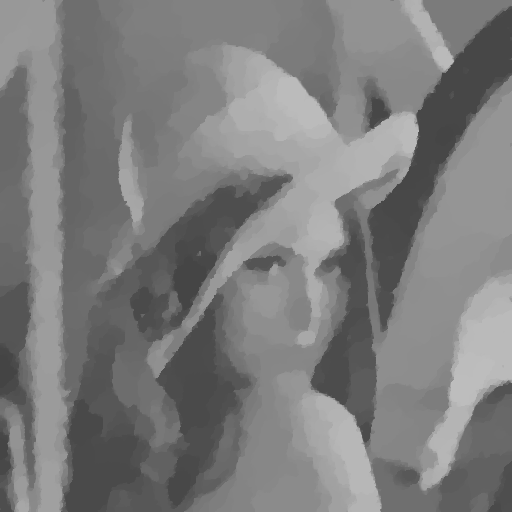
\includegraphics[width=\textwidth]{img/approximation/rof/rof_start/001lena.png}
                \caption{$\lambda = 0.01$}
            \end{subfigure}
            \caption{Approximation of the Lena image with the ROF Model. Again, the higher $\lambda$ the closer the outcome of the algrithm to the original image.}
        \label{fig:rof_lena_first_compare}
        \end{figure}

        It seemed not to be appropriable to go one one-thousandth steps and we already learned, that a small parameter does not lead to the desired results. We then turned our interest to the other extrem setting. We used the range from $0.1$ to $1$ in one-tenth steps. It not only lead to the perfect fit, it also produced good approximations $u$ of our input image $g$. This can also be seen in figure \ref{fig:rof_lena_second_compare}. We also want to show the table with some data like PSNR, iterations, energy and run-time.

        \begin{figure}[ht]
            \centering
            \begin{subfigure}[b]{0.18\textwidth}
                \includegraphics[width=\textwidth]{img/approximation/rof/rof_start/01lena.png}
                \caption{$\lambda = 0.1$}
            \end{subfigure}
            \begin{subfigure}[b]{0.18\textwidth}
                \includegraphics[width=\textwidth]{img/approximation/rof/rof_start/02lena.png}
                \caption{$\lambda = 0.2$}
            \end{subfigure}
            \begin{subfigure}[b]{0.18\textwidth}
                \includegraphics[width=\textwidth]{img/approximation/rof/rof_start/03lena.png}
                \caption{$\lambda = 0.3$}
            \end{subfigure}
            \begin{subfigure}[b]{0.18\textwidth}
                \includegraphics[width=\textwidth]{img/approximation/rof/rof_start/04lena.png}
                \caption{$\lambda = 0.4$}
            \end{subfigure}
            \begin{subfigure}[b]{0.18\textwidth}
                \includegraphics[width=\textwidth]{img/approximation/rof/rof_start/05lena.png}
                \caption{$\lambda = 0.5$}
            \end{subfigure}
            \begin{subfigure}[b]{0.18\textwidth}
                \includegraphics[width=\textwidth]{img/approximation/rof/rof_start/06lena.png}
                \caption{$\lambda = 0.6$}
            \end{subfigure}
            \begin{subfigure}[b]{0.18\textwidth}
                \includegraphics[width=\textwidth]{img/approximation/rof/rof_start/07lena.png}
                \caption{$\lambda = 0.7$}
            \end{subfigure}
            \begin{subfigure}[b]{0.18\textwidth}
                \includegraphics[width=\textwidth]{img/approximation/rof/rof_start/08lena.png}
                \caption{$\lambda = 0.8$}
            \end{subfigure}
            \begin{subfigure}[b]{0.18\textwidth}
                \includegraphics[width=\textwidth]{img/approximation/rof/rof_start/09lena.png}
                \caption{$\lambda = 0.9$}
            \end{subfigure}
            \begin{subfigure}[b]{0.18\textwidth}
                \includegraphics[width=\textwidth]{img/approximation/rof/rof_start/1lena.png}
                \caption{$\lambda = 1$}
            \end{subfigure}
            \caption{Approximation of the Lena image with the ROF Model. Again, the higher $\lambda$ the closer the outcome of the algrithm to the original image.}
        \label{fig:rof_lena_second_compare}
        \end{figure}

        Having a PSNR over 40 means, that we are extremely close to the original image. As discussed before, an image consists of data and noise and we seek to remove that noise from our images. We assumed to only consider approximation $u$, which have a PSNR less than 40. Then there were only the choices $0.1$ and $0.2$, but as the energy in the case $\lambda = 0.1$ was significantly smaller, we choose this $\lambda$ as our best estimate. We also ran some comparison for $\lambda = 0.09$ down to $\lambda = 0.06$, but nothing fitted better than this estimate.

        \begin{center}
            \begin{tabular}{| l | l | l | l | l | l |}
            \hline
            $\lambda$ & Iterations & Run-Time & MSE & PSNR & Energy \\ \hline\hline
            0.1 & 505 & 3.84 & 23 & 34 & 1,384,210 \\ \hline
            0.2 & 505 & 3.94 & 12 & 38 & 1,595,940 \\ \hline
            0.3 & 502 & 4.02 & 8 & 39 & 1,717,590 \\ \hline
            0.4 & 502 & 3.96 & 6 & 41 & 1,802,040 \\ \hline
            0.5 & 502 & 4.07 & 4 & 42 & 1,865,850 \\ \hline
            0.6 & 504 & 4.29 & 3 & 43 & 1,916,280 \\ \hline
            0.7 & 502 & 3.97 & 3 & 44 & 1,957,350 \\ \hline
            0.8 & 502 & 4.00 & 2 & 44 & 1,991,410 \\ \hline
            0.9 & 505 & 4.10 & 2 & 45 & 2,020,130 \\ \hline
            1.0 & 503 & 4.00 & 2 & 46 & 2,044,670 \\ \hline
            \end{tabular}
            \label{tab:best_fit_compare}
        \end{center}

    To the end of this subsection let us mention that in \cite{Chambolle10afirst-order} they proposed other estimates for $\lambda$, since they discretized the domain $\Omega$ by a factor $h_{N} = \frac{1}{N}$ and $h_{M} = \frac{1}{M}$, respectively. This factor enters our function in the discrete version of $\nabla$ and $\nabla^{T}$. It does not change the energy, since its a constant factor, but influences the scaling factor $\lambda$.

    \subsection{Best $\tau$ estimation}
    \label{sub:best_tau_estimation_rof}

        Unfortunattely, estimating the best $\tau$ is also a difficult task. It turns out, that $\tau$ couples with $\lambda$ and depends on the image itself. Finding a $\tau$, which delivers fast convergence is not impossible, but one has to guess instead of being able to verify a perfect estimate. We found, that for our perfect fit $\lambda = 0.1$ the best choice for the time-step can either be $\tau = 0.73$ or $\tau = 0.93$. We found these two values by running tests for $\tau$ starting at $0.01$ and inreasing it by $0.01$ till we reach the value $0.99$. For the tests we used three different images: Lena (grayscaled) and Hepburn, Van Gogh (both RGB). Since, there was no big difference in the estimated energy, we only focussed on iteration steps in our comparison. In

        \begin{table}
            \parbox{.9\linewidth}{
            \centering
                \begin{tabular}{| l | l | l | l | l | l | l | l | l |}
                    \hline
                    \multicolumn{5}{|c|}{Lena Image} & \multicolumn{4}{|c|}{Hepburn Image} \\ \hline\hline
                    No. & $\tau$ & Iterations & Run-Time & Energy & $\tau$ & Iterations & Run-Time & Energy \\ \hline
                    1 & 0.93 & 49 & 0.70 & 1.383.850 & 0.86 & 57 & 1.91 & 5.219.660 \\ \hline
                    2 & 0.73 & 52 & 0.75 & 1.384.130 & 0.84 & 65 & 2.08 & 5.219.470 \\ \hline
                    3 & 0.69 & 53 & 0.77 & 1.384.190 & 0.85 & 71 & 2.26 & 5.219.340 \\ \hline
                    4 & 0.61 & 65 & 0.94 & 1.384.200 & 0.93 & 72 & 2.34 & 5.219.120 \\ \hline
                    5 & 0.77 & 67 & 0.95 & 1.384.110 & 0.73 & 76 & 2.43 & 5.219.680 \\ \hline
                \end{tabular}
            }
            \hfill
            \parbox{\linewidth}{
            \centering
                \begin{tabular}{| l | l | l | l | l |}
                    \hline
                    \multicolumn{5}{|c|}{Van Gogh Image} \\ \hline\hline
                    No. & $\tau$ & Iterations & Run-Time & Energy \\ \hline
                    1 & 0.81 & 75 & 1.23 & 3.993.880 \\ \hline
                    2 & 0.85 & 78 & 1.34 & 3.993.780 \\ \hline
                    3 & 0.76 & 79 & 1.23 & 3.993.910 \\ \hline
                    4 & 0.73 & 93 & 1.45 & 3.993.770 \\ \hline
                     & & $\vdots$ & $\vdots$ & \\ \hline
                    15 & 0.93 & 123 & 1.79 & 3.993.660 \\ \hline
                \end{tabular}
            }
            \caption[My table caption for ROF and tau.]{Where the estimate $\tau = 0.93$ is under the five fastest approximations for the Lena and Hepburn image, it is only on fifteenth position using the Van Gogh image. Setting $\tau = 0.73$ gives us a better guarantee for fast convergence.}
            \label{tab:best_tau_compare}
        \end{table}

        We also tested some other images to see, if these two values are really the best option. It turned out, that it completely depends on the underlying image. In some cases convergence was attained within few iterations, but in other cases it took up to 200 iterations. Of course, this is not a large amount of iterations, but knowing nothing about the best time-step $\tau$ beforehand makes the proposed approach a bit incosistent. Nonetheless, having a stable framework like this to minimize the energy for the ROF model is a great approach and yields good approximations $u$ of the input images $g$.

\section{Image Approximation using the TVL1 Model} % (fold)
\label{sec:image_approximation_using_the_tvl1_model}

    We now turn our focus on the TVL1 model. Fortunately, we can adapt a lot of the previous section. The gradient operators and computation of the proximity operator for $F^{\ast}(p) = \delta_{P}(p)$ remain completely the same. Also the primal-dual algorithm with the extrapolation step are consistent and can be used. The only difference to the ROF model is the computation of $(\textnormal{Id} + \tau\,\partial\,G)^{-1}(\tilde{u})$. In equation \ref{eq:prox_g_tvl1} we showed, that it is of the form

        $$
            u = (\textnormal{Id} + \tau\,\partial\,G)^{-1}(\tilde{u}) \Longleftrightarrow u_{i, j} = 
                \begin{dcases*}
                    \tilde{u}_{i,j} - \tau\lambda & \textnormal{if\, $\tilde{u}_{i,j} - g_{i,j} > \tau\lambda$,} \\
                    \tilde{u}_{i,j} + \tau\lambda & \textnormal{if\, $\tilde{u}_{i,j} - g_{i,j} < - \tau\lambda$,} \\
                    g_{i, j} & \textnormal{if\, $|\tilde{u}_{i,j} - g_{i,j}| \le \tau\lambda$}.
                \end{dcases*}
        $$

    Now, the only thing we need to change in computing the function in algorithm \ref{alg:primal_descent} is the last line of code in the inner for-loop. In this line we compute the proximity operator for that change it to the one of the TVL1 model. We obtain:

        \begin{algorithm}[Primal Descent]
            Summarizing again in a function, we have
            \begin{lstlisting}
template<typename T>
void primal_desc(T* p_x, T* p_y, T* u, T* g, float tau, float lambda, int M, int N, int C) {
  T dx, dy, sum;
  int index;
  for (int k = 0; k < C; k++) {
    for (int i = 0; i < M; i++) {
      for (int j = 0; j < N; j++) {
        index = j + i * N + k * M * N;
        dx = (i+1<M ? p_x[index] : 0.f) -
             (i>0 ? p_x[j + (i-1) * N + k * M * N] : 0.f);
        dy = (j+1<N ? p_y[index] : 0.f) -
             (i>0 ? p_y[(j-1) + i * N + k * M * N] : 0.f);
        sum = tau * (dx + dy);
        sum += u[index];
        if (sum - g[i] > tau*lambda) u[i] = sum - tau*lambda;
        if (sum - g[i] < -tau*lambda) u[i] = sum + tau*lambda;
        if (fabs(sum - g[i]) <= tau*lambda) u[i] = g[i];
      }
    }
  }
}
            \end{lstlisting}
            where $C$ is the number of color channels and the template value $T$ is mostly used as float.
        \end{algorithm}

        This substitution is all it takes and we are ready to run the code and approximate the image $g$ by $u$.

        \subsection{Best $\lambda$ estimation} % (fold)
        \label{sub:best_lambda_estimation_tvl1}

            For the TVL1 model, estimating a good $\lambda$ was an easy task compared to the ROF model. The reason for this is, that in \cite{Chambolle10afirst-order} they proposed this model without the scaling factor $h$, like we did in this work. They already suggested to set $\lambda = 0.7$. We adapted this idea and tested all values from $0.1$ to $1$ by increasing $\lambda$ for each approximation by $0.1$. This evolution process is shown in figure \ref{fig:tvl1_lena_first_compare}. At the end, we can verify that $\lambda = 0.7$ is the best choice.
            
            \begin{figure}[ht]
            \centering
            \begin{subfigure}[b]{0.18\textwidth}
                \includegraphics[width=\textwidth]{img/approximation/tvl1/01lena.png}
                \caption{$\lambda = 0.1$}
            \end{subfigure}
            \begin{subfigure}[b]{0.18\textwidth}
                \includegraphics[width=\textwidth]{img/approximation/tvl1/02lena.png}
                \caption{$\lambda = 0.2$}
            \end{subfigure}
            \begin{subfigure}[b]{0.18\textwidth}
                \includegraphics[width=\textwidth]{img/approximation/tvl1/03lena.png}
                \caption{$\lambda = 0.3$}
            \end{subfigure}
            \begin{subfigure}[b]{0.18\textwidth}
                \includegraphics[width=\textwidth]{img/approximation/tvl1/04lena.png}
                \caption{$\lambda = 0.4$}
            \end{subfigure}
            \begin{subfigure}[b]{0.18\textwidth}
                \includegraphics[width=\textwidth]{img/approximation/tvl1/05lena.png}
                \caption{$\lambda = 0.5$}
            \end{subfigure}
            \begin{subfigure}[b]{0.18\textwidth}
                \includegraphics[width=\textwidth]{img/approximation/tvl1/06lena.png}
                \caption{$\lambda = 0.6$}
            \end{subfigure}
            \begin{subfigure}[b]{0.18\textwidth}
                \includegraphics[width=\textwidth]{img/approximation/tvl1/07lena.png}
                \caption{$\lambda = 0.7$}
            \end{subfigure}
            \begin{subfigure}[b]{0.18\textwidth}
                \includegraphics[width=\textwidth]{img/approximation/tvl1/08lena.png}
                \caption{$\lambda = 0.8$}
            \end{subfigure}
            \begin{subfigure}[b]{0.18\textwidth}
                \includegraphics[width=\textwidth]{img/approximation/rof/rof_start/09lena.png}
                \caption{$\lambda = 0.9$}
            \end{subfigure}
            \begin{subfigure}[b]{0.18\textwidth}
                \includegraphics[width=\textwidth]{img/approximation/rof/rof_start/1lena.png}
                \caption{$\lambda = 1$}
            \end{subfigure}
            \caption{Approximation of the Lena image with the TVL1 Model. Again, the higher $\lambda$ the closer the outcome of the algrithm to the original image.}
        \label{fig:tvl1_lena_first_compare}
        \end{figure}

        % subsection best_ (end)

        \subsection{Best $\tau$ estimation} % (fold)
        \label{sub:best_tau_estimation_tvl1}
            
            We applied the same procedure to estimate the best time-step parameter $\tau$ as in subsection \ref{sub:best_tau_estimation_rof}. We used again the images Lena, Hepburn and Van Gogh for the evaluation. There is only one parameter, which appeared under the sixth fastest convergence rates: $\tau = 0.98$, c.f. table \ref{tab:best_tau_compare_tvl1}.

            \begin{table}
                \parbox{\linewidth}{
                \centering
                    \begin{tabular}{| l | l | l | l |}
                        \hline
                        \multicolumn{4}{|c|}{Lena Image} \\ \hline\hline
                        $\tau$ & Iterations & Run-Time & Energy \\ \hline
                        0.98 & 245 & 2.27 & 1.576.060 \\ \hline
                        \multicolumn{4}{|c|}{Hepburn Image} \\ \hline\hline
                        $\tau$ & Iterations & Run-Time & Energy \\ \hline
                        0.98 & 328 & 7.17 & 5.635.150 \\ \hline
                        \multicolumn{4}{|c|}{Van Gogh Image} \\ \hline\hline
                        $\tau$ & Iterations & Run-Time & Energy \\ \hline
                        0.98 & 380 & 3.76 & 3.987.510 \\ \hline
                    \end{tabular}
                }
                \caption[My table caption for TVL1 and tau.]{The results for the best estimate $\tau = 0.98$.}
                \label{tab:best_tau_compare_tvl1}
            \end{table}

        % subsection best_tau_estimation (end)

        Testing this framework with other images lead again to different results. As before, finding a best fit for the time-step parameter is an impossible task.
    
% section image_approximation_using_the_tvl1_model (end)

\section{Approximation using the Real-Time Minimizer} % (fold)
\label{sec:approximation_using_the_real_time_minimizer}
    
    In the case of the real-time minimizer for the Mumford-Shah model we can again adapt most of the code from the ROF model. Since, the function $G$ is almost the same, except the scaling parameter $\frac{\lambda}{2}$, we only exchange one line of code. The line
        $$
            u[index] = (sum + tau * lambda * g[index]) / (1.f + tau * lambda);
        $$
    becomes
        $$
            u[index] = (sum + 2 * tau * g[index]) / (1.f + 2 * tau);.
        $$
    Everything else in algorithm \ref{alg:primal_descent} remains the same.

    In algorithm \ref{alg:dual_ascent} we only need to exchange two lines of code, where we take into account that the proximity operator for $R_{MS}^{\ast}(p)$ is computed by

        $$
            p = \bigg( \textnormal{Id} + \sigma \partial R_{MS}^{\ast} \bigg)^{-1}(\tilde{p}) \Longleftrightarrow p_{i,j} =
                \begin{dcases*}
                    \frac{\lambda}{\lambda + \sigma} \tilde{p}, & \textnormal{if $||\tilde{p}||_{2} \le \sqrt{\frac{\nu}{\lambda}\sigma(\sigma + 2\lambda)}$,} \\
                    0 & \textnormal{else.}
                \end{dcases*}
        $$

    We observe the following code:

        \begin{algorithm}[Dual Ascent]
            Summarizing this procedure in a function, we get
            \begin{lstlisting}
template<typename T>
void dual_asc(T* p_x, T* p_y, T* u_bar, float sigma, float lambda, float nu, int M, int N, int C) {
  T dx, dy;
  int index;
  aType factor = (2 * lambda) / (sigma + 2 * lambda);
  aType bound = sqrt((nu / lambda) * sigma * (sigma + 2 * lambda));
  for (int k = 0; k < C; k++) {
    for (int i = 0; i < M; i++) {
      for (int j = 0; j < N; j++) {
        index = j + i * N + k * M * N;
        dx = i+1<M ? u_bar[j + (i+1) * N + k * M * N]-u_bar[index] : 0;
        dy = j+1<N ? u_bar[(j+1) + i * N + k * M * N]-u_bar[index] : 0;
        dx = p_x[index] + sigma * dx;
        dy = p_y[index] + sigma * dy;
        p_x[index] = (dx*dx+dy*dy) <= bound ? factor * dx : 0;
        p_y[index] = (dx*dx+dy*dy) <= bound ? factor * dy : 0;
      }
    }
  }
}
            \end{lstlisting}
            where $C$ is the number of color channels and the template value $T$ is mostly used as float.
        \end{algorithm}

    As we used the second algorithm of section \ref{sec:a_firs_order_primal_dual_algorithm}, namely algorithm \ref{alg:f_star_or_g_uniformly_convex}, we additionally propose this version in C++ code:

    \begin{algorithm}[Primal-Dual Algorithm]
    \label{alg:primal_dual_2}
        In a function we have
        \begin{lstlisting}
template<typename T>
void RealTimeMinimizer(T* u, T* g, float lambda, float nu, int M, int N, int C) {
  float tau = 1.f / 4.f;
  float sigma = 1.f / 2.f;
  float theta = 2.f;
  T* u_bar = new T[M*N*C];
  T* u_prev = new T[M*N*C];
  T* p_x = new T[M*N*C];
  T* p_y = new T[M*N*C];
  
  void dual_asc(p_x, p_y, u_bar, sigma, lambda, nu, M, N, C);
  void primal_desc(p_x, p_y, u, g, tau, M, N, C);
  theta = (aType)1 / sqrt(1 + 4 * tau); tau *= theta; sigma /= theta;
  void extrapolation(u_bar, u, u_prev, theta, M, N, C);

  delete [] u_bar;
  delete [] u_prev;
  delete [] p_x;
  delete [] p_y;
}
        \end{lstlisting}
        where $C$ is the number of color channels and the template value $T$ is mostly used as float.
    \end{algorithm}

    It is left to evaluate a good $\lambda$ and $\nu$.

    \subsection{Best $\lambda$ and $\nu$ estimation} % (fold)
    \label{sub:best_parameter_estimation_rt}
        
        For this model we have two parameters which can be combined in a lot of ways. Finding parameters $\lambda$ and $\nu$ took several estimation steps. We will not provide the whole procedure of this process, since it could fill a huge amount of pages. But, we show and discuss the results of the estimation.

        \begin{center}
            \begin{tabular}{| l | l | l | l | l |}
            \hline
            $\lambda$ & $\nu$ & Iterations & Run-Time & Energy \\ \hline\hline
            2 & 0.02 & 260 & 1.72 & 527,42 \\ \hline
            2 & 0.03 & 260 & 1.71 & 579,89 \\ \hline
            20 & 0.03 & 260 & 2.05 & 1.746,89 \\ \hline
            20 & 0.04 & 260 & 1.95 & 1.895,69 \\ \hline
            500 & 0.07 & 260 & 1.93 & 3.094,23 \\ \hline
            500 & 0.08 & 260 & 1.81 & 3.132,59 \\ \hline
            \end{tabular}
            \label{tab:best_parameters_rt}
        \end{center}

        The corresponding images to the proposed values for $\lambda$ and $\nu$ can be seen in figure \ref{fig:realtime_lena_compare}.

        \begin{figure}[ht]
            \centering
            \begin{subfigure}[b]{0.32\textwidth}
                \includegraphics[width=\textwidth]{img/approximation/realtime/002lena2.png}
                \caption{$\alpha = 2, \lambda = 0.02$ (piecewise smooth)}
            \end{subfigure}
            \begin{subfigure}[b]{0.32\textwidth}
                \includegraphics[width=\textwidth]{img/approximation/realtime/003lena2.png}
                \caption{$\alpha = 2, \lambda = 0.03$ (piecewise constant)}
            \end{subfigure}
            \begin{subfigure}[b]{0.32\textwidth}
                \includegraphics[width=\textwidth]{img/approximation/realtime/003lena20.png}
                \caption{$\alpha = 20, \lambda = 0.03$ (piecewise constant)}
            \end{subfigure}
            \begin{subfigure}[b]{0.32\textwidth}
                \includegraphics[width=\textwidth]{img/approximation/realtime/004lena20.png}
                \caption{$\alpha = 20, \lambda = 0.04$ (piecewise smooth)}
            \end{subfigure}
            \begin{subfigure}[b]{0.32\textwidth}
                \includegraphics[width=\textwidth]{img/approximation/realtime/007lena500.png}
                \caption{$\alpha = 500, \lambda = 0.07$ (piecewise constant)}
            \end{subfigure}
            \begin{subfigure}[b]{0.32\textwidth}
                \includegraphics[width=\textwidth]{img/approximation/realtime/008lena500.png}
                \caption{$\alpha = 500, \lambda = 0.08$ (piecewise constant)}
            \end{subfigure}
            \caption{Approximation of Lena with the Mumford-Shah Model.}
        \label{fig:realtime_lena_compare}
        \end{figure}

        We tested the cases in which $\lambda = \{2, 20, 500\}$. Choosing $\lambda = 2$ yields to the piecewise smooth approximation $u$. It is close to the input image $g$ and the values set for $\nu$ seek for sharp edges in $u$. If $\lambda = 20$ the approximation turns slowly to a piecewise constant case. The output of the algorithm is still a quite smooth approximation, but some constant parts slightly appear. Again, $\nu$ controls the edges being sharp. The last case resembles the piecewise constant case. We see constant areas in the approximation. This setting is also useful for the cartooning case. For this, we then additionally propose a method for edge highlighting using the set $K_{MS}$.

        There is no need to find a good estimation of the time-step $\tau$, because this value is updated in each iteration seperately and is coupled with the parameter $\theta$.

    % subsection best_parameter_estimation_rt (end)

% section approximation_using_the_real_time_minimizer (end)

We proposed several image approximations $u$ of a input image $g$. Further, we showed good estimates for the parameters in each model and the time-step value $\tau$. We turn our interest no to one application to imaging, namely cartooning.

            % x = i + 1 < height ? p_x[j + i * width + k * height * width] : 0.0;
            %     x_minus_one = i > 0 ? p_x[j + (i-1) * width + k * height * width] : 0.0;


%         \begin{figure}[ht]
%             \centering
%             \begin{subfigure}[b]{0.45\textwidth}
%                 \includegraphics[width=\textwidth]{img/approximation/rof/006hepburn.png}
%                 \caption{$\lambda = 0.06$}
%             \end{subfigure}
%             \begin{subfigure}[b]{0.45\textwidth}
%                 \includegraphics[width=\textwidth]{img/approximation/rof/007hepburn.png}
%                 \caption{$\lambda = 0.07$}
%             \end{subfigure}
%             \begin{subfigure}[b]{0.45\textwidth}
%                 \includegraphics[width=\textwidth]{img/approximation/rof/009hepburn.png}
%                 \caption{$\lambda = 0.09$}
%             \end{subfigure}
%             \begin{subfigure}[b]{0.45\textwidth}
%                 \includegraphics[width=\textwidth]{img/approximation/rof/01hepburn.png}
%                 \caption{$\lambda = 0.1$}
%             \end{subfigure}
%             \begin{subfigure}[b]{0.45\textwidth}
%                 \includegraphics[width=\textwidth]{img/approximation/rof/06hepburn.png}
%                 \caption{$\lambda = 0.6$}
%             \end{subfigure}
%             \begin{subfigure}[b]{0.45\textwidth}
%                 \includegraphics[width=\textwidth]{img/approximation/rof/09hepburn.png}
%                 \caption{$\lambda = 0.9$}
%             \end{subfigure}
%             \caption{Approximation of Audrey Hepburn with the ROF Model. The higher $\lambda$ the closer the outcome of the algrithm to the original image.}
%         \label{fig:rof_hepburn_compare}
%         \end{figure}
%     % subsection image_approximation_using_the_rof_model (end)
% % section image_approximation (end)

% \begin{figure}[ht]
%     \centering
%     \begin{subfigure}[b]{0.45\textwidth}
%         \includegraphics[width=\textwidth]{img/approximation/tvl1/06hepburn.png}
%         \caption{$\lambda = 0.6$}
%     \end{subfigure}
%     \begin{subfigure}[b]{0.45\textwidth}
%         \includegraphics[width=\textwidth]{img/approximation/tvl1/07hepburn.png}
%         \caption{$\lambda = 0.7$}
%     \end{subfigure}
%     \begin{subfigure}[b]{0.45\textwidth}
%         \includegraphics[width=\textwidth]{img/approximation/tvl1/08hepburn.png}
%         \caption{$\lambda = 0.8$}
%     \end{subfigure}
%     \begin{subfigure}[b]{0.45\textwidth}
%         \includegraphics[width=\textwidth]{img/approximation/tvl1/09hepburn.png}
%         \caption{$\lambda = 0.9$}
%     \end{subfigure}
%     \caption{Approximation of Audrey Hepburn with the TVL1 Model. The higher $\lambda$ the closer the outcome of the algrithm to the original image.}
% \label{fig:tvl1_hepburn_compare}
% \end{figure}

% \begin{figure}[ht]
%     \centering
%     \begin{subfigure}[b]{0.4\textwidth}
%         \includegraphics[width=\textwidth]{img/approximation/tvl1/06lena.png}
%         \caption{$\lambda = 0.6$}
%     \end{subfigure}
%     \begin{subfigure}[b]{0.4\textwidth}
%         \includegraphics[width=\textwidth]{img/approximation/tvl1/07lena.png}
%         \caption{$\lambda = 0.7$}
%     \end{subfigure}
%     \begin{subfigure}[b]{0.4\textwidth}
%         \includegraphics[width=\textwidth]{img/approximation/tvl1/08lena.png}
%         \caption{$\lambda = 0.8$}
%     \end{subfigure}
%     \begin{subfigure}[b]{0.4\textwidth}
%         \includegraphics[width=\textwidth]{img/approximation/tvl1/09lena.png}
%         \caption{$\lambda = 0.9$}
%     \end{subfigure}
%     \caption{Approximation of the Lena image with the TVL1 Model. Again, the higher $\lambda$ the closer the outcome of the algrithm to the original image.}
% \label{fig:tvl1_lena_compare}
% \end{figure}

% \begin{figure}[ht]
%     \centering
%     \begin{subfigure}[b]{0.45\textwidth}
%         \includegraphics[width=\textwidth]{img/approximation/realtime/003hepburn20.png}
%         \caption{$\alpha = 20, \lambda = 0.03$ (piecewise smooth)}
%     \end{subfigure}
%     \begin{subfigure}[b]{0.45\textwidth}
%         \includegraphics[width=\textwidth]{img/approximation/realtime/05hepburn500.png}
%         \caption{$\alpha = 500, \lambda = 0.5$ (piecewise constant)}
%     \end{subfigure}
%     \begin{subfigure}[b]{0.45\textwidth}
%         \includegraphics[width=\textwidth]{img/approximation/realtime/004hepburn20.png}
%         \caption{$\alpha = 20, \lambda = 0.04$ (piecewise smooth)}
%     \end{subfigure}
%     \begin{subfigure}[b]{0.45\textwidth}
%         \includegraphics[width=\textwidth]{img/approximation/realtime/07hepburn500.png}
%         \caption{$\alpha = 500, \lambda = 0.7$ (piecewise constant)}
%     \end{subfigure}
%     \caption{Approximation of Audrey Hepburn with the Mumford-Shah Model. The higher $\lambda$ the closer the outcome of the algrithm to the original image.}
% \label{fig:realtime_hepburn_compare}
% \end{figure}

% \begin{figure}[ht]
%     \centering
%     \begin{subfigure}[b]{0.4\textwidth}
%         \includegraphics[width=\textwidth]{img/approximation/realtime/003lena20.png}
%         \caption{$\alpha = 20, \lambda = 0.03$ (piecewise smooth)}
%     \end{subfigure}
%     \begin{subfigure}[b]{0.4\textwidth}
%         \includegraphics[width=\textwidth]{img/approximation/realtime/007lena500.png}
%         \caption{$\alpha = 500, \lambda = 0.5$ (piecewise constant)}
%     \end{subfigure}
%     \begin{subfigure}[b]{0.4\textwidth}
%         \includegraphics[width=\textwidth]{img/approximation/realtime/004lena20.png}
%         \caption{$\alpha = 20, \lambda = 0.04$ (piecewise smooth)}
%     \end{subfigure}
%     \begin{subfigure}[b]{0.4\textwidth}
%         \includegraphics[width=\textwidth]{img/approximation/realtime/008lena500.png}
%         \caption{$\alpha = 500, \lambda = 0.7$ (piecewise constant)}
%     \end{subfigure}
%     \caption{Approximation of the Lena image with the Mumford-Shah Model. Again, the higher $\lambda$ the closer the outcome of the algrithm to the original image.}
% \label{fig:realtime_lena_compare}
% \end{figure}

% \begin{figure}[ht]
%     \centering
%     \begin{center}
%         \rotatebox{90}{$\lambda = 0.005$}
%         \begin{subfigure}[b]{0.21\textwidth}
%             \includegraphics[width=\textwidth]{img/evolution/rof/0005hepburn.png}
%         \end{subfigure}
%         \rotatebox{90}{$\lambda = 0.2$}
%         \begin{subfigure}[b]{0.21\textwidth}
%             \includegraphics[width=\textwidth]{img/evolution/tvl1/02hepburn.png}
%         \end{subfigure}
%         \rotatebox{90}{$\lambda = 0.01$}
%         \begin{subfigure}[b]{0.21\textwidth}
%             \includegraphics[width=\textwidth]{img/evolution/realtime/001hepburn20.png}
%         \end{subfigure}
%         \rotatebox{90}{$\lambda = 0.1$}
%         \begin{subfigure}[b]{0.21\textwidth}
%             \includegraphics[width=\textwidth]{img/evolution/realtime/01hepburn500.png}
%         \end{subfigure}
%     \end{center}
%     \begin{center}
%         \rotatebox{90}{$\lambda = 0.007$}
%         \begin{subfigure}[b]{0.21\textwidth}
%             \includegraphics[width=\textwidth]{img/evolution/rof/0007hepburn.png}
%         \end{subfigure}
%         \rotatebox{90}{$\lambda = 0.3$}
%         \begin{subfigure}[b]{0.21\textwidth}
%             \includegraphics[width=\textwidth]{img/evolution/tvl1/03hepburn.png}
%         \end{subfigure}
%         \rotatebox{90}{$\lambda = 0.03$}
%         \begin{subfigure}[b]{0.21\textwidth}
%             \includegraphics[width=\textwidth]{img/evolution/realtime/003hepburn20.png}
%         \end{subfigure}
%         \rotatebox{90}{$\lambda = 0.3$}
%         \begin{subfigure}[b]{0.21\textwidth}
%             \includegraphics[width=\textwidth]{img/evolution/realtime/03hepburn500.png}
%         \end{subfigure}
%     \end{center}
%     \begin{center}
%         \rotatebox{90}{$\lambda = 0.009$}
%         \begin{subfigure}[b]{0.21\textwidth}
%             \includegraphics[width=\textwidth]{img/evolution/rof/0009hepburn.png}
%         \end{subfigure}
%         \rotatebox{90}{$\lambda = 0.4$}
%         \begin{subfigure}[b]{0.21\textwidth}
%             \includegraphics[width=\textwidth]{img/evolution/tvl1/04hepburn.png}
%         \end{subfigure}
%         \rotatebox{90}{$\lambda = 0.05$}
%         \begin{subfigure}[b]{0.21\textwidth}
%             \includegraphics[width=\textwidth]{img/evolution/realtime/005hepburn20.png}
%         \end{subfigure}
%         \rotatebox{90}{$\lambda = 0.5$}
%         \begin{subfigure}[b]{0.21\textwidth}
%             \includegraphics[width=\textwidth]{img/evolution/realtime/05hepburn500.png}
%         \end{subfigure}
%     \end{center}
%     \begin{center}
%         \rotatebox{90}{$\lambda = 0.02$}
%         \begin{subfigure}[b]{0.21\textwidth}
%             \includegraphics[width=\textwidth]{img/evolution/rof/002hepburn.png}
%         \end{subfigure}
%         \rotatebox{90}{$\lambda = 0.5$}
%         \begin{subfigure}[b]{0.21\textwidth}
%             \includegraphics[width=\textwidth]{img/evolution/tvl1/05hepburn.png}
%         \end{subfigure}
%         \rotatebox{90}{$\lambda = 0.07$}
%         \begin{subfigure}[b]{0.21\textwidth}
%             \includegraphics[width=\textwidth]{img/evolution/realtime/007hepburn20.png}
%         \end{subfigure}
%         \rotatebox{90}{$\lambda = 0.7$}
%         \begin{subfigure}[b]{0.21\textwidth}
%             \includegraphics[width=\textwidth]{img/evolution/realtime/07hepburn500.png}
%         \end{subfigure}
%     \end{center}
%     \begin{center}
%         \rotatebox{90}{$\lambda = 0.04$}
%         \begin{subfigure}[b]{0.21\textwidth}
%             \includegraphics[width=\textwidth]{img/evolution/rof/004hepburn.png}
%         \end{subfigure}
%         \rotatebox{90}{$\lambda = 0.6$}
%         \begin{subfigure}[b]{0.21\textwidth}
%             \includegraphics[width=\textwidth]{img/evolution/tvl1/06hepburn.png}
%         \end{subfigure}
%         \rotatebox{90}{$\lambda = 0.09$}
%         \begin{subfigure}[b]{0.21\textwidth}
%             \includegraphics[width=\textwidth]{img/evolution/realtime/009hepburn20.png}
%         \end{subfigure}
%         \rotatebox{90}{$\lambda = 0.9$}
%         \begin{subfigure}[b]{0.21\textwidth}
%             \includegraphics[width=\textwidth]{img/evolution/realtime/09hepburn500.png}
%         \end{subfigure}
%     \end{center}
%     \caption{Evolution of the Audrey Hepburn image, whereas the left column shows the ROF Model, the second column the TVL1 Model, the third column resembles the piecewise smooth approximation of the Mumford-Shah Model with the real-time minimizer with $\alpha = 20$. The right column shows the piecewise constant case of the last mentioned algorithm with $\alpha = 500$.}
% \end{figure}

% \begin{figure}[ht]
% \centering
% \begin{center}
%     \rotatebox{90}{$\lambda = 0.005$}
%     \begin{subfigure}[b]{0.19\textwidth}
%         \includegraphics[width=\textwidth]{img/evolution/rof/0005lena.png}
%     \end{subfigure}
%     \rotatebox{90}{$\lambda = 0.2$}
%     \begin{subfigure}[b]{0.19\textwidth}
%         \includegraphics[width=\textwidth]{img/evolution/tvl1/02lena.png}
%     \end{subfigure}
%     \rotatebox{90}{$\lambda = 0.01$}
%     \begin{subfigure}[b]{0.19\textwidth}
%         \includegraphics[width=\textwidth]{img/evolution/realtime/001lena20.png}
%     \end{subfigure}
%     \rotatebox{90}{$\lambda = 0.01$}
%     \begin{subfigure}[b]{0.19\textwidth}
%         \includegraphics[width=\textwidth]{img/evolution/realtime/001lena500.png}
%     \end{subfigure}
% \end{center}
% \begin{center}
%     \rotatebox{90}{$\lambda = 0.007$}
%     \begin{subfigure}[b]{0.19\textwidth}
%         \includegraphics[width=\textwidth]{img/evolution/rof/0007lena.png}
%     \end{subfigure}
%     \rotatebox{90}{$\lambda = 0.3$}
%     \begin{subfigure}[b]{0.19\textwidth}
%         \includegraphics[width=\textwidth]{img/evolution/tvl1/03lena.png}
%     \end{subfigure}
%     \rotatebox{90}{$\lambda = 0.03$}
%     \begin{subfigure}[b]{0.19\textwidth}
%         \includegraphics[width=\textwidth]{img/evolution/realtime/003lena20.png}
%     \end{subfigure}
%     \rotatebox{90}{$\lambda = 0.03$}
%     \begin{subfigure}[b]{0.19\textwidth}
%         \includegraphics[width=\textwidth]{img/evolution/realtime/003lena500.png}
%     \end{subfigure}
% \end{center}
% \begin{center}
%     \rotatebox{90}{$\lambda = 0.009$}
%     \begin{subfigure}[b]{0.19\textwidth}
%         \includegraphics[width=\textwidth]{img/evolution/rof/0009lena.png}
%     \end{subfigure}
%     \rotatebox{90}{$\lambda = 0.4$}
%     \begin{subfigure}[b]{0.19\textwidth}
%         \includegraphics[width=\textwidth]{img/evolution/tvl1/04lena.png}
%     \end{subfigure}
%     \rotatebox{90}{$\lambda = 0.05$}
%     \begin{subfigure}[b]{0.19\textwidth}
%         \includegraphics[width=\textwidth]{img/evolution/realtime/005lena20.png}
%     \end{subfigure}
%     \rotatebox{90}{$\lambda = 0.05$}
%     \begin{subfigure}[b]{0.19\textwidth}
%         \includegraphics[width=\textwidth]{img/evolution/realtime/005lena500.png}
%     \end{subfigure}
% \end{center}
% \begin{center}
%     \rotatebox{90}{$\lambda = 0.02$}
%     \begin{subfigure}[b]{0.19\textwidth}
%         \includegraphics[width=\textwidth]{img/evolution/rof/002lena.png}
%     \end{subfigure}
%     \rotatebox{90}{$\lambda = 0.5$}
%     \begin{subfigure}[b]{0.19\textwidth}
%         \includegraphics[width=\textwidth]{img/evolution/tvl1/05lena.png}
%     \end{subfigure}
%     \rotatebox{90}{$\lambda = 0.07$}
%     \begin{subfigure}[b]{0.19\textwidth}
%         \includegraphics[width=\textwidth]{img/evolution/realtime/007lena20.png}
%     \end{subfigure}
%     \rotatebox{90}{$\lambda = 0.07$}
%     \begin{subfigure}[b]{0.19\textwidth}
%         \includegraphics[width=\textwidth]{img/evolution/realtime/007lena500.png}
%     \end{subfigure}
% \end{center}
% \begin{center}
%     \rotatebox{90}{$\lambda = 0.04$}
%     \begin{subfigure}[b]{0.19\textwidth}
%         \includegraphics[width=\textwidth]{img/evolution/rof/004lena.png}
%     \end{subfigure}
%     \rotatebox{90}{$\lambda = 0.6$}
%     \begin{subfigure}[b]{0.19\textwidth}
%         \includegraphics[width=\textwidth]{img/evolution/tvl1/06lena.png}
%     \end{subfigure}
%     \rotatebox{90}{$\lambda = 0.09$}
%     \begin{subfigure}[b]{0.19\textwidth}
%         \includegraphics[width=\textwidth]{img/evolution/realtime/009lena20.png}
%     \end{subfigure}
%     \rotatebox{90}{$\lambda = 0.09$}
%     \begin{subfigure}[b]{0.19\textwidth}
%         \includegraphics[width=\textwidth]{img/evolution/realtime/009lena500.png}
%     \end{subfigure}
% \end{center}
% \caption{Evolution of the Lena image, whereas the left column shows the ROF Model, the second column the TVL1 Model, the third column resembles the piecewise smooth approximation of the Mumford-Shah Model with the real-time minimizer with $\alpha = 20$. The right column shows the piecewise constant case of the last mentioned algorithm with $\alpha = 500$.}
% \end{figure}
    % \section{Image Cartooning} % (fold)
\label{sec:image_cartooning}
    
    In this section we present a technique to turn an input image $g$ into a cartooned image $u$. For this we will make use of the ROF Model, TVL1 Model and most of all the real-time minimizer for the Mumford-Shah Function, presented in section \ref{sec:the_mumford_shah_functional}. Using the model of Rudin, Osher and Fatemi and the TVL1 Model meant for us to find the right parameter $\lambda$ to smooth the image enough, but still preserve edges. We will exchange the data fidelity term $G$, by another term $G^{q}_{\gamma}$. This leads to a nice cartoon representation of our image. For this, we first propose the new data fidelity term and then we compute the corresponding proximity operator, which depends on the function $G^{q}_{\gamma}$.

    \subsection{A new data fidelity term} % (fold)
    \label{sub:a_new_data_fidelity_term}

        Recalling the Mumford-Shah energy function we had
            $$
                E_{MS}(u) = ||u - g||_{2}^{2} + \sum_{i = 1}^{N} \sum_{j = 1}^{M} \min(\lambda |(\nabla u)_{i,j}|, \nu),
            $$
        where we set the data fidelity term to $G(u) = ||u - g||_{2}^{2}$. The idea for cartooning is now to replace $G$ with a function $G^{q}_{\gamma}$ defined by
            \begin{equation}
                G^{q}_{\gamma}(u) := ||u - g||_{2}^{2} + \gamma ||u - u^{\textnormal{prev}}||_{q}^{q}.
                \label{eq:ms_new_regularizer}
            \end{equation}
        Here, $u^{\textnormal{prev}}$ is the $u$, which was obtained in the previous iteration, hence the notation. The additional $l_{q}$ regularization aims to handle the tradeoff between the current and the previous estimate of $u$. It forces $u$ not to change too much during the iterations process. But as mentioned above, we need to compute the proximity operator with respect to the new function $G^{q}_{\gamma}$. Using again \ref{eq:proximity_operator_reloaded}, we obtain

            \begin{equation}
                u = (\textnormal{Id} + \tau \partial G^{q}_{\gamma})^{-1}(\tilde{u}) = \arg \min_{u \in X} \frac{||u - \tilde{u}||_{2}^{2}}{2} + \tau \left( ||u - g||_{2}^{2} + \gamma ||u - u^{\textnormal{prev}}||_{q}^{q} \right).
                \label{eq:prox_new_data_fidelity_term}
            \end{equation}

        As one can see, the new proximity operator is dependent on how the norm in the additional term is chosen. We are looking at the cases where we have $q = 1$ and $q = 2$. In the appendix of \cite{Strekalovskiy-Cremers-eccv14} they suggest using $q = 1.5$ and therefore also compute the proximal operator. In our tests, this did not have that big impact, for that we choose to use the $l_{1}$ and $l_{2}$ norm, respectively.

        Let us first consider the case where $q = 2$. Then we obtain for the proximal operator
            \begin{eqnarray}
                u = (\textnormal{Id} + \tau \partial G^{q}_{\gamma})^{-1}(\tilde{u}) &=& \arg \min_{u \in X} \frac{||u - \tilde{u}||_{2}^{2}}{2} + \tau \left( ||u - g||_{2}^{2} + \gamma ||u - u^{\textnormal{prev}}||_{2}^{2} \right) \notag \\
                &\Longleftrightarrow& 0 \in \partial \bigg( \frac{||u - \tilde{u}||_{2}^{2}}{2} + \tau \left( ||u - g||_{2}^{2} + \gamma ||u - u^{\textnormal{prev}}||_{2}^{2} \right) \bigg)\notag \\
                &\Longleftrightarrow& 0 \in u - \tilde{u} + 2\tau(u - g) + 2\tau\gamma (u - u^{\textnormal{prev}}) \notag \\
                &\Longleftrightarrow& u \big( 1 + 2\tau + 2\tau\gamma \big) = \tilde{u} + 2\tau g + 2\tau\gamma u^{\textnormal{prev}} \notag \\
                &\Longleftrightarrow& u = \frac{\tilde{u} + 2\tau g + 2\tau\gamma u^{\textnormal{prev}}}{1 + 2\tau + 2\tau\gamma} \notag
            \end{eqnarray}
        Overall, we obtain pointwise for all $i = 1, ..., N$ and $j = 1, ..., M$
            \begin{equation}
                u_{i, j} = \frac{\tilde{u}_{i, j} + 2\tau g_{i, j} + 2\tau\gamma u^{\textnormal{prev}_{i, j}}}{1 + 2\tau + 2\tau\gamma}
                \label{eq:prox_d_q_two}
            \end{equation}

        The other option was to set $q = 1$. In this case we obtain the non-differentiable $l_{1}$ norm and we need to make use of the subgradient. We need to do a case analysis. For this, let $y_{i}$ be the subgradient of the term $||u - u^{\textnormal{prev}}||_{1}$ in the i-th component with $y_{i} \in [-1, 1]$. Then we get with the the equations for the proximity operator:
            \begin{eqnarray}
                u = (\textnormal{Id} + \tau \partial G^{q}_{\gamma})^{-1}(\tilde{u}) &=& \arg \min_{u \in X} \frac{||u - \tilde{u}||_{2}^{2}}{2} + \tau \left( ||u - g||_{2}^{2} + \gamma ||u - u^{\textnormal{prev}}||_{1}^{1} \right) \notag \\
                &\Longleftrightarrow& 0 \in \partial \bigg( \frac{||u - \tilde{u}||_{2}^{2}}{2} + \tau \left( ||u - g||_{2}^{2} + \gamma ||u - u^{\textnormal{prev}}||_{1} \right) \bigg)\notag \\
                &\Longleftrightarrow& 0 \in u - \tilde{u} + 2\tau (u - g) + \tau\gamma y \notag
            \end{eqnarray}
        We will look at the i-the row of this equation.
        \begin{enumerate}
            \item Consider the first case and assume that $u_{i} - u^{\textnormal{prev}}_{i} > 0$. Then clearly, $y_{i} = 1$ and
                \begin{eqnarray}
                    0 \in u_{i} - \tilde{u}_{i} + 2\tau (u_{i} - g_{i}) + \tau\gamma &\Longleftrightarrow& u_{i} (1 + 2\tau) = \tilde{u}_{i} + 2\tau g_{i} - \tau\gamma \notag \\
                    &\Longleftrightarrow& u_{i} = \frac{\tilde{u}_{i} + 2\tau g_{i} - \tau\gamma}{1 + 2\tau}. \notag
                \end{eqnarray}
            Then, the last equation implies
                \begin{eqnarray}
                    \frac{\tilde{u}_{i} + 2\tau g_{i} - \tau\gamma}{1 + 2\tau} - u^{\textnormal{prev}} > 0 &\Longleftrightarrow& \tilde{u}_{i} + 2\tau g_{i} - \tau\gamma - u^{\textnormal{prev}} (1 + 2\tau) > 0 \notag \\
                    &\Longleftrightarrow& \tilde{u}_{i} + 2\tau g_{i} - u^{\textnormal{prev}} (1 + 2\tau) > \tau\gamma.
                \end{eqnarray}
            \item Assuming that $u_{i} - u^{\textnormal{prev}}_{i} < 0$ leads to a similar expression, but we need to exchange the sign in front of the term $\tau\gamma$, since in this case it holds that $y_{i} = -1$. Overall, we obtain
                $$
                    u_{i} = \frac{\tilde{u}_{i} + 2\tau g_{i} + \tau\gamma}{1 + 2\tau}.
                $$
            As in 1. we can compute
                \begin{eqnarray}
                    \frac{\tilde{u}_{i} + 2\tau g_{i} + \tau\gamma}{1 + 2\tau} - u^{\textnormal{prev}} < 0 &\Longleftrightarrow& \tilde{u}_{i} + 2\tau g_{i} + \tau\gamma - u^{\textnormal{prev}} (1 + 2\tau) < 0 \notag \\
                    &\Longleftrightarrow& \tilde{u}_{i} + 2\tau g_{i} - u^{\textnormal{prev}} (1 + 2\tau) < -\tau\gamma.
                \end{eqnarray}
            \item In the last case we assume that the equality $u_{i} = u^{\textnormal{prev}}_{i}$ holds. Then we have that $y_{i} \in [-1, 1]$ can be set arbitrary. To show in which case this setting holds we plug $y_{i}$ into the equation, set $u_{i} = u^{\textnormal{prev}}_{i}$ and observe
                \begin{eqnarray}
                    0 \in u^{\textnormal{prev}}_{i} - \tilde{u}_{i} + 2\tau (u^{\textnormal{prev}}_{i} - g_{i}) + \tau\gamma y_{i} &\Longleftrightarrow& u^{\textnormal{prev}}_{i} - \tilde{u}_{i} + 2\tau (u^{\textnormal{prev}}_{i} - g_{i}) = - \tau\gamma y_{i} \notag \\
                    &\Longleftrightarrow& \tilde{u}_{i} - u^{\textnormal{prev}}_{i} (1 + 2\tau) + 2\tau g_{i} = \tau\gamma y_{i} \notag \\
                    &\Longleftrightarrow& |\tilde{u}_{i} - u^{\textnormal{prev}}_{i} (1 + 2\tau) + 2\tau g_{i}| = |\tau\gamma y_{i}| \le \tau \gamma \notag
                \end{eqnarray}
        \end{enumerate}

        Overall, we have the following representation of the proximity operator to this problem:
            \begin{subequations}
                \begin{align}
                    u &= (\textnormal{Id} + \tau\,\partial\,G^{q}_{\gamma})^{-1}(\tilde{u}) \Longleftrightarrow \\
                    u_{i, j} &=
                        \begin{dcases*}
                            \frac{\tilde{u}_{i,j} + 2\tau g_{i,j} - \tau\gamma}{1 + 2\tau} & \textnormal{if\, $\tilde{u}_{i,j} + 2\tau g_{i,j} - u^{\textnormal{prev}} (1 + 2\tau) > \tau\gamma$,} \\
                            \frac{\tilde{u}_{i,j} + 2\tau g_{i,j} + \tau\gamma}{1 + 2\tau} & \textnormal{if\, $\tilde{u}_{i,j} + 2\tau g_{i,j} - u^{\textnormal{prev}} (1 + 2\tau) < -\tau\gamma$,} \\
                            u^{\textnormal{prev}}_{i,j} & \textnormal{if\, $|\tilde{u}_{i,j} - u^{\textnormal{prev}}_{i,j} (1 + 2\tau) + 2\tau g_{i,j}| \le \tau\gamma$},
                        \end{dcases*}
                \label{eq:prox_d_q_one}
                \end{align}
            \end{subequations}
        for all $i = 1, ..., N$, $j = 1, ..., M$.

    % subsection a_new_data_fidelity_term (end)

    \subsection{Edge Highlighting} % (fold)
    \label{sub:edge_highlighting}
        
        Another idea Strekalovskiy and Cremers proposed in \cite{Strekalovskiy-Cremers-eccv14} was to use the edge set $K_{MS}$ in order to highlight edges in the smoothed images.

        Assume that $x \in K_{MS}$ then we have $|\nabla u(x)| \ge \sqrt{\frac{\nu}{\lambda}}$ by definition. This notation is equivalent to setting
            $$
                \frac{|\nabla u(x)|}{\sqrt{\frac{\nu}{\lambda}}} \ge 1.
            $$
        Further, we have by discretizing the operator $\nabla$ with forward differences that
            $$
                |\nabla u(x)| = \max_{|u(x)| \le 1} |\nabla u(x)| = \max_{|x| \le 1} |\frac{u(x+\delta x) - u(x)}{\delta x}|.
            $$
        This means we have $|\nabla u(x)| \le \sqrt{2}$ and for that
            $$
                1 \le \frac{|\nabla u(x)|}{\sqrt{\frac{\nu}{\lambda}}} \le \frac{\sqrt{2}}{\sqrt{\frac{\nu}{\lambda}}}.
            $$
        Applying the logarithm to each of the terms we get
            $$
                0 \le \log \bigg( \frac{|\nabla u(x)|}{\sqrt{\frac{\nu}{\lambda}}} \bigg) \le \log \bigg( \frac{\sqrt{2}}{\sqrt{\frac{\nu}{\lambda}}} \bigg).
            $$
        If we now divide each term by the last one, we observe
            $$
                0 \le \frac{\log \bigg( \frac{|\nabla u(x)|}{\sqrt{\frac{\nu}{\lambda}}} \bigg)}{\log \bigg( \frac{\sqrt{2}}{\sqrt{\frac{\nu}{\lambda}}} \bigg)} \le 1.
            $$
        With these calculations, we now define a $v \in [0, 1]$ by
            $$
                v := \frac{\log \bigg( \frac{|\nabla u(x)|}{\sqrt{\frac{\nu}{\lambda}}} \bigg)}{\log \bigg( \frac{\sqrt{2}}{\sqrt{\frac{\nu}{\lambda}}} \bigg)},
            $$
        then, since $\nu$ and $\lambda$ are constant values, this parameter $v$ only increases if $|\nabla u(x)|$ increases and decreases if $|\nabla u(x)|$ decreases. For this reason $v$ can serve as an edge indicator. Then the idea proposed by \cite{Strekalovskiy-Cremers-eccv14} is to multiply each RGB value $u(x)$ by
            $$
                1 - v \in [0, 1],
            $$
        if $x \in K_{MS}$. On the other hand, if $x \notin K_{MS}$ the value $u(x)$ will not be changed. Then points in the imaged domain $\Omega$ with strong edges are painted darker, as those where we do not find edges.

    % subsection edge_highlighting (end)

    \subsection{Image Comparison} % (fold)
    \label{sub:image_comparison}

        In this subsection we want to present solutions of the three models: ROF, TVL1 and real-time Mumford-Shah minimizer. We will compare run-time of the models - on a CPU and GPU - and provide the best estimations for the parameters $\lambda, \nu$ and $\gamma$. We start with the ROF Model:

        \begin{figure}[ht]
            \centering
            \begin{subfigure}[b]{0.45\textwidth}
                \includegraphics[width=\textwidth]{img/cartooning/rof/001hepburn.png}
                \caption{$\lambda = 0.01$}
            \end{subfigure}
            \begin{subfigure}[b]{0.45\textwidth}
                \includegraphics[width=\textwidth]{img/cartooning/tvl1/035hepburn.png}
                \caption{$\lambda = 0.35$}
            \end{subfigure}
            \caption[Cartooning Comparison of Hepburn using ROF and TVL1]{Comparison of cartooning applying the ROF Model (left) and the TVL1 Model (right) to the Audrey Hepburn image}
        \label{fig:cartooning_comparison_hepburn}
        \end{figure}

        \begin{figure}[ht]
            \centering
            \begin{subfigure}[b]{0.45\textwidth}
                \includegraphics[width=\textwidth]{img/cartooning/rof/001lena.png}
                \caption{$\lambda = 0.01$}
            \end{subfigure}
            \begin{subfigure}[b]{0.45\textwidth}
                \includegraphics[width=\textwidth]{img/cartooning/tvl1/035lena.png}
                \caption{$\lambda = 0.35$}
            \end{subfigure}
            \caption[Cartooning Comparison of Lena using ROF and TVL1]{Comparison of cartooning applying the ROF Model (left) and the TVL1 Model (right) to the Lena image}
        \label{fig:cartooning_comparison_lena}
        \end{figure}

        One can see that the difference of these two models becomes visible at the edges. As the ROF Model really smoothes the image and provides pretty good cartooned images, the TVL1 Model preserves more edges and details in the images. But, what both models have in common: the cartoon images do not fit the imagination one has when thinking about cartoons. Therefore, we not only applied the real-time minimzer for the Mumford-Shah model to the images, we also made use of the above data fidelity term $G^{q}_{\gamma}$ and the method for edge highlighting. We start with $q = 1$.

        \begin{figure}[ht]
            \centering
            \begin{subfigure}[b]{0.45\textwidth}
                \includegraphics[width=\textwidth]{img/cartooning/realtime/104hepburn500.png}
                \caption{$\alpha = 500, \lambda = 0.4, \gamma = 1$}
            \end{subfigure}
            \begin{subfigure}[b]{0.45\textwidth}
                \includegraphics[width=\textwidth]{img/cartooning/realtime/1004hepburn500.png}
                \caption{$\alpha = 500, \lambda = 0.4, \gamma = 10$}
            \end{subfigure}
            \begin{subfigure}[b]{0.45\textwidth}
                \includegraphics[width=\textwidth]{img/cartooning/realtime/2004hepburn500.png}
                \caption{$\alpha = 500, \lambda = 0.4, \gamma = 20$}
            \end{subfigure}
            \begin{subfigure}[b]{0.45\textwidth}
                \includegraphics[width=\textwidth]{img/cartooning/realtime/5005hepburn500.png}
                \caption{$\alpha = 500, \lambda = 0.5, \gamma = 50$}
            \end{subfigure}
            \caption{Cartooning of.}
        \label{fig:cartooning_hepburn_realtime}
        \end{figure}

        By estimating the best fits for our parameters we ran a huge amount of tests. Using the framework presented for the Mumford-Shah Model, we observed a lot of possible images and chose the ones, which fitted best for us. Finding nicely cartooned images for the ROF and TVL1 Model, respectively, was a harder task. We obtained also a large number of images, but only a few fitted to be considered as cartoon images. Overall, the real-time minimizer is the model to choose, if one seeks for cartooned images or movies.

    \subsection{Computational Comparison} % (fold)
    \label{sub:computational_comparison}
        
        In this part of the section we present the run-times for the three models for the best fitted parameters for cartooning. We also provide the best time-step parameter $\tau$ for the ROF and TVL1 model, the iterations to convergence and the final (minimal) energy of the model. Further, we discuss some implementation issues and the comparison of running the algorithms on a CPU and GPU.

        For this computational comparison we use the Audrey Hepburn image with the parameters presented in subsection \ref{sub:image_comparison}. For the Mumford-Shah Model the parameter $\tau$ is set to $0.25$ by definition of th proposed algorithm in section \ref{sec:a_firs_order_primal_dual_algorithm}.
        \begin{center}
            \begin{tabular}{| l | l | l | l | l | l |}
            \hline
            Model & $\tau$ & CPU time & GPU time & Iterations & Energy  \\ \hline
            ROF & 0.25 &  &  &  &  \\ \hline
            ROF & 0.5 &  &  &  &  \\ \hline
            ROF & 0.97 &  &  &  &  \\ \hline
            TVL1 & 0.25 &  &  &  &  \\ \hline
            TVL1 & 0.5 &  &  &  &  \\ \hline
            TVL1 & 0.97 &  &  &  &  \\ \hline
            Mumford-Shah & 0.25 &  &  &  &  \\ \hline
            Mumford-Shah & 0.25 &  &  &  &  \\ \hline
            Mumford-Shah & 0.25 &  &  &  &  \\ \hline
            \end{tabular}
        \end{center}
    % subsection computational_comparison (end)

    % subsection image_comparison (end)

% section image_cartooning (end)
    % \section{Image Denoising} % (fold)
\label{sec:image_denoising}
    
    Denoising images is a hard task. As discussed before, an image $g$ consists of data and noisy. Our goal is to remove the noise from an input image $g$ and get a smooth approximation $u$. We find different kinds of noise on images. The two most common are Gaussian noise and the so called salt and pepper noise. Where Gaussian noise is relatively easy to remove, salt and pepper noise is more robust since it resembles extrem values on images. 
% section image_denoising (end)

\begin{figure}[ht]
    \centering
    \begin{subfigure}[b]{0.45\textwidth}
        \includegraphics[width=\textwidth]{img/denoising/gauss_noise/rof/002lena.png}
        \caption{$\lambda = 0.02$}
    \end{subfigure}
    \begin{subfigure}[b]{0.45\textwidth}
        \includegraphics[width=\textwidth]{img/denoising/gauss_noise/rof/003lena.png}
        \caption{$\lambda = 0.03$}
    \end{subfigure}
    \caption{Denoising of Salt and Pepper noise of the Lena image with the ROF Model.}
\label{fig:denoising_lena_rof_gauss}
\end{figure}

\begin{figure}[ht]
    \centering
    \begin{subfigure}[b]{0.45\textwidth}
        \includegraphics[width=\textwidth]{img/denoising/gauss_noise/tvl1/05lena.png}
        \caption{$\lambda = 0.5$}
    \end{subfigure}
    \begin{subfigure}[b]{0.45\textwidth}
        \includegraphics[width=\textwidth]{img/denoising/gauss_noise/tvl1/06lena.png}
        \caption{$\lambda = 0.6$}
    \end{subfigure}
    \begin{subfigure}[b]{0.45\textwidth}
        \includegraphics[width=\textwidth]{img/denoising/gauss_noise/tvl1/07lena.png}
        \caption{$\lambda = 0.7$}
    \end{subfigure}
    \begin{subfigure}[b]{0.45\textwidth}
        \includegraphics[width=\textwidth]{img/denoising/gauss_noise/tvl1/08lena.png}
        \caption{$\lambda = 0.8$}
    \end{subfigure}
    \caption{Denoising of Gaussian noise of the Lena image with the TVL1 Model.}
\label{fig:denoising_lena_tvl1_gauss}
\end{figure}

\begin{figure}[ht]
    \centering
    \begin{subfigure}[b]{0.45\textwidth}
        \includegraphics[width=\textwidth]{img/denoising/salt_and_pepper_noise/rof/0007lena.png}
        \caption{$\lambda = 0.007$}
    \end{subfigure}
    \begin{subfigure}[b]{0.45\textwidth}
        \includegraphics[width=\textwidth]{img/denoising/salt_and_pepper_noise/rof/0008lena.png}
        \caption{$\lambda = 0.008$}
    \end{subfigure}
    \caption{Denoising of Salt and Pepper noise of the Lena image with the ROF Model.}
\label{fig:denoising_lena_rof_sap}
\end{figure}

\begin{figure}[ht]
    \centering
    \begin{subfigure}[b]{0.45\textwidth}
        \includegraphics[width=\textwidth]{img/denoising/salt_and_pepper_noise/tvl1/05lena.png}
        \caption{$\lambda = 0.5$}
    \end{subfigure}
    \begin{subfigure}[b]{0.45\textwidth}
        \includegraphics[width=\textwidth]{img/denoising/salt_and_pepper_noise/tvl1/06lena.png}
        \caption{$\lambda = 0.6$}
    \end{subfigure}
    \begin{subfigure}[b]{0.45\textwidth}
        \includegraphics[width=\textwidth]{img/denoising/salt_and_pepper_noise/tvl1/07lena.png}
        \caption{$\lambda = 0.7$}
    \end{subfigure}
    \begin{subfigure}[b]{0.45\textwidth}
        \includegraphics[width=\textwidth]{img/denoising/salt_and_pepper_noise/tvl1/08lena.png}
        \caption{$\lambda = 0.8$}
    \end{subfigure}
    \caption{Denoising of Salt and Pepper noise of the Lena image with the TVL1 Model.}
\label{fig:denoising_lena_tvl1_sap}
\end{figure}
    % \begin{figure}[ht]
    \centering
    \begin{subfigure}[b]{0.45\textwidth}
        \includegraphics[width=\textwidth]{img/inpainting/rof/006lena.png}
        \caption{$\lambda = 0.06$}
    \end{subfigure}
    \begin{subfigure}[b]{0.45\textwidth}
        \includegraphics[width=\textwidth]{img/inpainting/rof/007lena.png}
        \caption{$\lambda = 0.07$}
    \end{subfigure}
    \begin{subfigure}[b]{0.45\textwidth}
        \includegraphics[width=\textwidth]{img/inpainting/rof/009lena.png}
        \caption{$\lambda = 0.09$}
    \end{subfigure}
    \begin{subfigure}[b]{0.45\textwidth}
        \includegraphics[width=\textwidth]{img/inpainting/rof/01lena.png}
        \caption{$\lambda = 0.1$}
    \end{subfigure}
    \caption{Inpainting of Lena image with the ROF Model.}
\label{fig:inpainting_lena_rof}
\end{figure}

% chapter applications_to_imaging (end)

% \chapter{Conclusion} % (fold)
% \label{cha:conclusion}

    % \input{19_conclusion}

% chapter conclusion (end)

\bibliographystyle{plain}
\bibliography{bibliography}

\end{document}